%%%%%%%%%%%%%%%%%%%%%%%%%%%%%%%%%%%%%%%%%
% Masters/Doctoral Thesis 
% LaTeX Template
% Version 2.5 (27/8/17)
%
% This template was downloaded from:
% http://www.LaTeXTemplates.com
%
% Version 2.x major modifications by:
% Vel (vel@latextemplates.com)
%
% This template is based on a template by:
% Steve Gunn (http://users.ecs.soton.ac.uk/srg/softwaretools/document/templates/)
% Sunil Patel (http://www.sunilpatel.co.uk/thesis-template/)
%
% Template license:
% CC BY-NC-SA 3.0 (http://creativecommons.org/licenses/by-nc-sa/3.0/)
%
%%%%%%%%%%%%%%%%%%%%%%%%%%%%%%%%%%%%%%%%%

%----------------------------------------------------------------------------------------
%	PACKAGES AND OTHER DOCUMENT CONFIGURATIONS
%----------------------------------------------------------------------------------------

\documentclass[
11pt, % The default document font size, options: 10pt, 11pt, 12pt
%oneside, % Two side (alternating margins) for binding by default, uncomment to switch to one side
english, % ngerman for German
singlespacing, % Single line spacing, alternatives: onehalfspacing or doublespacing
%draft, % Uncomment to enable draft mode (no pictures, no links, overfull hboxes indicated)
%nolistspacing, % If the document is onehalfspacing or doublespacing, uncomment this to set spacing in lists to single
%liststotoc, % Uncomment to add the list of figures/tables/etc to the table of contents
%toctotoc, % Uncomment to add the main table of contents to the table of contents
%parskip, % Uncomment to add space between paragraphs
%nohyperref, % Uncomment to not load the hyperref package
headsepline, % Uncomment to get a line under the header
%chapterinoneline, % Uncomment to place the chapter title next to the number on one line
%consistentlayout, % Uncomment to change the layout of the declaration, abstract and acknowledgements pages to match the default layout
]{MastersDoctoralThesis} % The class file specifying the document structure
\usepackage{color}
\usepackage[svgnames]{xcolor}
\usepackage{listings}
\usepackage{textcomp}
\usepackage{float}
\usepackage{amsthm}
\definecolor{listinggray}{gray}{0.9}

\definecolor{bggrey}{grey}{0.095}

\lstset{language=R,
    basicstyle=\ttfamily,
    stringstyle=\color{DarkGreen},
    otherkeywords={0,1,2,3,4,5,6,7,8,9},
    morekeywords={TRUE,FALSE},
    deletekeywords={data,frame,length,as,character},
    %keywordstyle=[1]{\color{blue}},
    %morekeywords = [1]{select},
    commentstyle=\color{black},
    backgroundcolor = \color{listinggray},
    showstringspaces = false
}



\usepackage[utf8]{inputenc} % Required for inputting international characters
\usepackage[T1]{fontenc} % Output font encoding for international characters

\usepackage{mathpazo} % Use the Palatino font by default

\usepackage[backend=bibtex,style=authoryear,natbib=true]{biblatex} % Use the bibtex backend with the authoryear citation style (which resembles APA)

\addbibresource{example.bib} % The filename of the bibliography

\usepackage[autostyle=true]{csquotes} % Required to generate language-dependent quotes in the bibliography

\usepackage{hyperref}
\usepackage{tcolorbox}
%----------------------------------------------------------------------------------------
%	MARGIN SETTINGS
%----------------------------------------------------------------------------------------

\geometry{
	paper=a4paper, % Change to letterpaper for US letter
	inner=2.5cm, % Inner margin
	outer=3.8cm, % Outer margin
	bindingoffset=.5cm, % Binding offset
	top=1.5cm, % Top margin
	bottom=1.5cm, % Bottom margin
	%showframe, % Uncomment to show how the type block is set on the page
}

%----------------------------------------------------------------------------------------
%	THESIS INFORMATION
%----------------------------------------------------------------------------------------

\thesistitle{Survey statistics in a database} % Your thesis title, this is used in the title and abstract, print it elsewhere with \ttitle
\supervisor{Professor Thomas \textsc{Lumley}} % Your supervisor's name, this is used in the title page, print it elsewhere with \supname
\examiner{} % Your examiner's name, this is not currently used anywhere in the template, print it elsewhere with \examname
\degree{Bachelor of Science (Honours)} % Your degree name, this is used in the title page and abstract, print it elsewhere with \degreename
\author{Charco \textsc{Hui}} % Your name, this is used in the title page and abstract, print it elsewhere with \authorname
\addresses{} % Your address, this is not currently used anywhere in the template, print it elsewhere with \addressname
\subject{Biological Sciences} % Your subject area, this is not currently used anywhere in the template, print it elsewhere with \subjectname
\keywords{} % Keywords for your thesis, this is not currently used anywhere in the template, print it elsewhere with \keywordnames
\university{\href{http://www.auckland.ac.nz}{The University of Auckland}} % Your university's name and URL, this is used in the title page and abstract, print it elsewhere with \univname
\department{\href{https://www.stat.auckland.ac.nz/en.html}{Department of Statistics}} % Your department's name and URL, this is used in the title page and abstract, print it elsewhere with \deptname
%\group{\href{http://researchgroup.university.com}{Research Group Name}} % Your research group's name and URL, this is used in the title page, print it elsewhere with \groupname
%\faculty{\href{http://faculty.university.com}{Faculty Name}} % Your faculty's name and URL, this is used in the title page and abstract, print it elsewhere with \facname

\AtBeginDocument{
\hypersetup{pdftitle=\ttitle} % Set the PDF's title to your title
\hypersetup{pdfauthor=\authorname} % Set the PDF's author to your name
\hypersetup{pdfkeywords=\keywordnames} % Set the PDF's keywords to your keywords
}
%\graphicspath{{/img}}
\begin{document}

\frontmatter % Use roman page numbering style (i, ii, iii, iv...) for the pre-content pages

\pagestyle{plain} % Default to the plain heading style until the thesis style is called for the body content

%----------------------------------------------------------------------------------------
%	TITLE PAGE
%----------------------------------------------------------------------------------------

\begin{titlepage}
\begin{center}

\vspace*{.06\textheight}
{\scshape\LARGE \univname\par}\vspace{1.5cm} % University name
\textsc{\Large Honours Project}\\[0.5cm] % Thesis type

\HRule \\[0.4cm] % Horizontal line
{\huge \bfseries \ttitle\par}\vspace{0.4cm} % Thesis title
\HRule \\[1.5cm] % Horizontal line
 
\begin{minipage}[t]{0.4\textwidth}
\begin{flushleft} \large
\emph{Author:}\\
\href{https://github.com/chrk623}{\authorname} % Author name - remove the \href bracket to remove the link
\end{flushleft}
\end{minipage}
\begin{minipage}[t]{0.4\textwidth}
\begin{flushright} \large
\emph{Supervisor:} \\
\href{https://www.stat.auckland.ac.nz/people/tlum005}{\supname} % Supervisor name - remove the \href bracket to remove the link  
\end{flushright}
\end{minipage}\\[3cm]
 

\includegraphics[scale=0.1]{Latex/img/uoalogo.png}

\vfill

\large \textit{A thesis submitted in fulfilment of the requirements\\ for the degree of \degreename}\\[0.3cm] % University requirement text
\textit{in the}\\[0.4cm]
\groupname\\\deptname\\[2cm] % Research group name and department name
 
\vfill

{\large June 5, 2017}\\[4cm] % Date
%\includegraphics{Logo} % University/department logo - uncomment to place it
 
\vfill
\end{center}
\end{titlepage}

%----------------------------------------------------------------------------------------
%	ABSTRACT PAGE
%----------------------------------------------------------------------------------------

\begin{abstract}
%\addchaptertocentry{\abstractname} % Add the abstract to the table of contents
%The Thesis Abstract is written here (and usually kept to just this page). The page is kept centered %vertically so can expand into the blank space above the title too\ldots
\addchaptertocentry{\abstractname} % Add the acknowledgements to the table of contents
Multistage surveys can rise to moderately large data sets (tens of millions of rows).  Most current software for survey analysis reads the data into memory, the {\bf survey} package in {\sf R} provides fairly comprehensive analysis features for complex surveys which are small enough to fit into memory easily, however, most of the computations can actually be expressed as database operations. There is already a similar approach with the {\bf sqlsurvey} package in {\sf R} which performs substantial computation in {\sf SQL} in the database, importing only small summary tables into {\sf R}, this approach scales to very large surveys such as the American Community Survey and the Nationwide Emergency Department Sample, but this approach causes compatibility issues with different types of databases. Therefore, in this project I will work on implementing {\sf R} functions and testing some survey computations using the {\bf dplyr} and {\bf dbplyr} {\sf R} package as a efficient and portable database interface.

\end{abstract}

%----------------------------------------------------------------------------------------
%	ACKNOWLEDGEMENTS
%----------------------------------------------------------------------------------------

\begin{acknowledgements}
\addchaptertocentry{\acknowledgementname} % Add the acknowledgements to the table of contents
I would like to acknowledge my supervisor, Professor Thomas Lumley with my deepest appreciation. I would like to thank him for his patience in sharing his expertise, without his help, this project would not be possible. \\

Lastly, i would like to thank my friends and family for their continuous support.
\end{acknowledgements}

%----------------------------------------------------------------------------------------
%	LIST OF CONTENTS/FIGURES/TABLES PAGES
%----------------------------------------------------------------------------------------

\tableofcontents % Prints the main table of contents

\listoffigures % Prints the list of figures

%\listoftables % Prints the list of tables

%----------------------------------------------------------------------------------------
%	ABBREVIATIONS
%----------------------------------------------------------------------------------------

% \begin{abbreviations}{ll} % Include a list of abbreviations (a table of two columns)

% \textbf{LAH} & \textbf{L}ist \textbf{A}bbreviations \textbf{H}ere\\
% \textbf{WSF} & \textbf{W}hat (it) \textbf{S}tands \textbf{F}or\\

% \end{abbreviations}

%----------------------------------------------------------------------------------------
%	PHYSICAL CONSTANTS/OTHER DEFINITIONS
%----------------------------------------------------------------------------------------

% \begin{constants}{lr@{${}={}$}l} % The list of physical constants is a three column table

% % The \SI{}{} command is provided by the siunitx package, see its documentation for instructions on how to use it

% Speed of Light & $c_{0}$ & \SI{2.99792458e8}{\meter\per\second} (exact)\\
% %Constant Name & $Symbol$ & $Constant Value$ with units\\

% \end{constants}

%----------------------------------------------------------------------------------------
%	SYMBOLS
%----------------------------------------------------------------------------------------

% \begin{symbols}{lll} % Include a list of Symbols (a three column table)

% $a$ & distance & \si{\meter} \\
% $P$ & power & \si{\watt} (\si{\joule\per\second}) \\
% %Symbol & Name & Unit \\

% \addlinespace % Gap to separate the Roman symbols from the Greek

% $\omega$ & angular frequency & \si{\radian} \\

% \end{symbols}

%----------------------------------------------------------------------------------------
%	DEDICATION
%----------------------------------------------------------------------------------------

% \dedicatory{For/Dedicated to/To my\ldots} 

%----------------------------------------------------------------------------------------
%	THESIS CONTENT - CHAPTERS
%----------------------------------------------------------------------------------------

\mainmatter % Begin numeric (1,2,3...) page numbering

\pagestyle{thesis} % Return the page headers back to the "thesis" style

% Include the chapters of the thesis as separate files from the Chapters folder
% Uncomment the lines as you write the chapters

% Chapter Template

\chapter{Introduction} % Main chapter title

\label{Introduction} % Change X to a consecutive number; for referencing this chapter elsewhere, use \ref{ChapterX}

%----------------------------------------------------------------------------------------
%	SECTION 1
%----------------------------------------------------------------------------------------

\section{Background}\label{c1.1}

Currently, there is already a {\bf survey} package  \citep{surveypackage} in {\sf R} which is at a stable production status, it provides survey analysis, including graphics, estimation and inference. It also supports both replicate-weight and Taylor linearisation standard errors, and can efficiently handle multistage stratified designs without replacements. However, it requires the data sets to be stored in a data frame in memory. For most survey data sets this is not a problem, however, nowadays there are a number of large survey data sets, for example the American Community Survey (ACS) includes 3,000,000 people per year, and the Nationwide Emergency Department Sample (NEDS) includes more than 25,000,000 hospital visit records per year. \\

In {\sf R}, there are currently two approaches to analyse survey data sets in a database. The first is to use the {\bf survey} package, with its database back-end function, the data sets can be loaded into memory without any problem, but the time to analysis the data may not be promising when the data sets are too large.\\

Another approach is to perform as much computation as possible directly in the database, so that only small bits of data or numbers are transferred into memory when necessary. This approach is more efficient but is less flexible, since mathematics and statistical operations are limited in a database. Another advantage of this approach is that if the database is powerful, then the computation would be faster than just using a standard laptop or desktop. 

The second approach is implemented in the {\bf sqlsurvey} {\sf R} package \citep{sqlsurveypackage}}, however, codes which communicates with the databases are written in "hand-written {\sf SQL} code". Therefore, it would be hard to maintain and would cause compatibility issues between different types of databases. Not only codes may look different, there is also a major inconsistency in evaluating the code, for example dealing with missing values. Despite the attempt of standardising the {\sf SQL} standards between multiple companies, issues of portability still remains.\\

The better approach to analyse survey data sets in a database would be to use the {\sf R} packages {\bf dplyr} \citep{dplyrpackage} and {\bf dbplyr} \citep{dbplyrpackage} as a database interface. Since these packages are maintained by experts at Rstudio, it is likely that these packages are more stable than others, bug fixes and updates would also be quick. Most importantly, it is more portable where its compatibility extends to powerful databases back ends like PostgreSQL and Google BigQuery. So, this project will implement a set of functions to analyse survey data sets with the second approach, named {\bf svydb}, and evaluate its speed on large survey data sets.

\section{Survey data in SQL}
As mentioned in section \ref{c1.1}, when we are analysing large survey data sets, it would be more feasible to do it in a database. Some commonly used survey statistics are survey mean, survey total, summaries and regression.\\

Survey totals, means and summaries can be easily computed in a database, since it only requires simple arithmetic like summing, multiplications, divisions along with some grouping. 

Regression may require a bit more work, since it requires matrix operations which are not supported in {\sf SQL}, however by loading a few chunks of small matrices into memory, it can still be easily implemented in a database, since after all regression coefficients and their variances only requires sums and multiplications.\\

More details of the calculations and difficulties will be discussed later on in Chapter \ref{c2}.

\section{Coding with {\bf dplyr} and {\bf dbplyr}}

\subsection{Introduction to dplyr} \label{c1.2.1}
The {\bf dplyr} package was implemented to manipulate, clean and construct data. With this package, data manipulation and data exploration can be done easily and quickly, since they are written in a computationally efficient manner. 

The package contains a few common data manipulating functions such as selecting specific columns, arranging or creating new columns, filtering rows, merging data (joins) and summarising data by groups. Other features such as simple statistics operations are also included in the package.

\subsection{Pipes}
The pipe operator ({\ttfamily \%>\%}) first appeared in {\bf magrittr} package \citep{magrittrpackage}, and is created to make codes more readable.
The pipe operator inputs the object on the left-hand side of the pipe into the function on right-hand side. Some basic piping are as follows:

\begin{itemize}

\item {\ttfamily x \%>\% f} is equivalent to {\ttfamily f(x).}

\item {\ttfamily x \%>\% f(y)} is equivalent to {\ttfamily f(x, y).} 

\end{itemize}
\\
\vspace{10}
It is rather useful when we have multiple steps while we are transforming data sets, because naturally we read from left to right. For example, with traditional coding, reading is always from inside out,
\begin{lstlisting}
> x = sample(10)
> summary(diff(exp(floor(cos(x)))))
\end{lstlisting}
with piping, it is much easier to read,
\begin{lstlisting}
> x %>% cos() %>% floor() %>% exp() %>% diff() 
    %>% summary() 
\end{lstlisting}
\\
\vspace{10}
Though the pipe has its advantages, there are also times that it is not useful. It would not be useful when the intermediate variables are needed or when the intermediate variables require heavy computation.

\subsection{dplyr's SQL compatibility (dbplyr)}
As mentioned in section \ref{c1.2.1}, there are six basic functions in {\bf dplyr}. These functions are all related to the basic {\sf SQL} queries.

%https://www.listendata.com/2016/08/dplyr-tutorial.html
\begin{center}
\begin{tabular}{ |l|l|l|l| } 
\hline
\textbf{dplyr Function} & \textbf{Description} & \textbf{Equivalent SQL} \\
\hline
select() & Selecting columns (variables) & SELECT \\ 
filter () & Filter (subset) rows. & WHERE \\ 
group\_by() & Group the data & GROUP BY \\ 
arrange() & Sort the data & ORDER BY \\ 
join() & Joining tables & JOIN \\ 
mutate() & Creating New Variables (Columns) & COLUMN ALIAS \\ 
\hline
\end{tabular}
\end{center}

With {\bf dbplyr}, when these {\bf dplyr} functions are applied onto a sql table, they automatically translate itself into {\sf SQL} queries. For example,

\begin{lstlisting}
> mtdb %>% select(mpg, gear) %>% group_by(gear) %>% 
    summarise(sum_mpg = sum(mpg)) %>% head(3) %>% 
    show_query()
 
 # <SQL>
 # SELECT "gear", SUM("mpg") AS "sum_mpg"
 # FROM (SELECT "mpg" AS "mpg", "gear" AS "gear"
 # FROM "mtcars") "gaecowztcc"
 # GROUP BY "gear"
 # LIMIT 3
\end{lstlisting}
With this approach, {\bf dplyr} does not actually do any work, its job is only to translate the codes into {\sf SQL} and gives the database instructions. Another advantage of this method is that the intermediate variables between the pipes only builds up the query and does not get evaluated nor is stored anywhere. 

\subsection{Quasi-quotation}
Programming with {\bf dplyr} relies on a concept called the quasi-quotation, also known as non-standard evaluation, it means that while we are doing some evaluation with {\bf dplyr} in {\sf R}, we are not using {\sf R}'s standard evaluation method. For example, with {\sf R}'s standard method, 

\begin{lstlisting}
test_func = function(x, y){
    x + y
}  
> x1 = 1; x2 = 2
> test_func(x1, x2)
\end{lstlisting}
{\sf R} looks for the variables {\ttfamily x1} and {\ttfamily x2} in the environment, evaluates them and input their values into the function {\ttfamily test\_func}. \\

However, while programming in {\bf dplyr},
\begin{lstlisting}
> mtcars %>% select(mpg)
\end{lstlisting}
The variable {\ttfamily mpg} is a variable in the data set and cannot be found in the environment, it is quoted and evaluated in a non standard way.\\

Though, it might look useful to use this non-standard evaluation method, but it is more difficult to program with, for example while writing a function,

\begin{lstlisting}
test_fun2 = function(data, x){
    data %>% select(x) %>% head(2)
}
> test_fun2(mtcars, mpg)
# Error: `x` must resolve to integer column positions, 
# not a list 
\end{lstlisting}

Since {\bf dplyr} does not evaluate in the standard way, we cannot just pass a variable in like the standard method. We will need to quote it with the {\ttfamily quo()} or {\ttfamily enquo()} function.

\begin{lstlisting}
test_fun2 = function(data, x){
    x = enquo(x)
    data %>% select(!!x) %>% head(2) %>% tbl_df()
}
> test_fun2(mtcars, mpg)
    
#    mpg
#* <dbl>
#1    21
#2    21
\end{lstlisting}
{\ttfamily enquo()} allows us to quote the variable resulting in a quosure where it contains its expression along with an evaluation environment, so we can pass it into the {\ttfamily select()} function, and {\ttfamily !!} (bang bang) allows us to unquote the variable at evaluation. \\

There are also other similar functions to help us overcome the difficulties while programming with  {\bf dplyr}, like {\ttfamily quos()}, {\ttfamily sym()} and {\ttfamily quo\_name()} which are used in different situations.

\subsection{Common issues while coding with dplyr in a database}

\begin{itemize}
    \item No factor types in {\sf SQL}.
    \item Difficult to code with quasi-quotation.
    \item Cannot do row-wise operations due to the lazy interface. That is, the data sets within a database in {\sf R} will not be loaded into memory unless required.
    \item No matrix operations.
    \item No base {\sf R} functions. 
    \item No distributions.
    \item Inconsistent availability of functions between databases.
\end{itemize}

%\newpage

\section{Layout}

In chapter \ref{c2}, estimation methods and functions will be discussed, and in chapter \ref{c3}, graphics. 

In chapter \ref{c4}, speed of database-based and memory-based implementations will be compared,  chapter \ref{c5} discuss the usability of the functions, and lastly, a discussion in chapter \ref{c6}.
%\include{Chapters/Chapter1}
% Chapter 2

\chapter{Methodology} \label{c2} % Main chapter title

%\label{Chapter1} % For referencing the chapter elsewhere, use \ref{Chapter1} 

%----------------------------------------------------------------------------------------

% Define some commands to keep the formatting separated from the content 
\newcommand{\keyword}[1]{\textbf{#1}}
\newcommand{\tabhead}[1]{\textbf{#1}}
\newcommand{\code}[1]{\texttt{#1}}
\newcommand{\file}[1]{\texttt{\bfseries#1}}
\newcommand{\option}[1]{\texttt{\itshape#1}}

%----------------------------------------------------------------------------------------
\section{Survey Design} \label{c2.1}
When analysing survey data sets in the {\bf survey} package, a survey design ({\bf svydesign()}) is always required. The survey design object combines the data set and all the survey design information needed to analyse it. These objects are used by the survey modelling and summary functions.\\

The set of functions that {\bf surveydb} provides also adapted this concept but with a few modifications, it uses the {\bf R6} \citep{R6package} class system which is encapsulated object orientation programming and is different to the standard {\bf S3} and {\bf S4} in base {\sf R} which uses functional object orientation programming. The main difference between the two is that {\bf S3} and {\bf S4} methods and objects are separate and in {\bf R6}, object contains methods and data. \\

The advantage of encapsulated object orientation programming is that information within the objects are not computed unless it is needed, for example when the sum of all sampling weights are needed, we can compute it by using a method within the object and the value also updates when it's been called on a subset of the object.

\begin{lstlisting}
> nh.dbsurv = svydbdesign(st = SDMVSTRA, wt = WTMEC2YR, 
    id = SDMVPSU, data = nhdb)
> nh.dbsurv$getwt()
[1] 306590681

> nh.dbsurv$subset(Race3 == 3)$getwt()
[1] 192721267
\end{lstlisting}

Therefore, it is much more time efficient than creating a survey design that contains all the information, since the user may not need every information within the object. \\

% Another advantage of this approach is that there will not be any extra generic methods that can be called directly by the user, because these methods are designed specifically for a type of object and usually it should not be called directly by the user.


The {\ttfamily svydbdesign()} function, has four basic arguments,
\begin{center}
    {\ttfamily svydbdesign(st = NULL, id = NULL, wt, data)}
\end{center}

\begin{itemize}
\item $st$ = Column name specifying the strata column. $NULL$ for no strata. 

\item $id$ = Column name specifying the cluster column. $NULL$ for no cluster. 

\item $wt$ = Column name specifying the sampling weights column.

\item $data$ = A data frame or sql table of the survey data set.
\end{itemize}

\\

When the {\ttfamily svydb.design} object is called directly, a brief description of the design will be displayed.

\begin{lstlisting}
> nh.dbsurv
svydb.design, 9756 observation(s), 31 Clusters
\end{lstlisting}

\\

Functions within the {\bf svydb.design} object for users to use are,

\begin{lstlisting}
Classes 'svydb.design', 'R6' <svydb.design>
.
.
clone: function (deep = FALSE) 
getmh: function () 
getwt: function () 
subset: function (..., logical = T) 
subset_rows: function (from, to) 
\end{lstlisting}


\begin{itemize}
\item $clone()$ = Create a clone of the object.

\item $getmh()$ = A table indicating strata and cluster information.

\item $getwt()$ = Compute the sum of the sampling weights.

\item $subset()$ = Subset the design by conditions, similar to $base::subset$. \\
                    e.g.({\ttfamilyd design\$subset(Race3 == 3)} 

\item $subset\_rows()$ = Subset the design by rows. 

e.g.({\ttfamily design\$subset\_rows(1, 100)} )

\end{itemize}

%----------------------------------------------------------------------------------------
\newpage

\section{Population Total} \label{c2:tot} \label{c2.2}
%http://essedunet.nsd.uib.no/cms/topics/weight/3/1.html



The function {\ttfamily svydbtotal()} was designed to estimate the population total in {\sf R} by using {\bf dplyr}, it is compatible with data frames and sql tables and was designed to do as much computation as possible in a database.\\

In the function {\ttfamily svydbtotal()}, the total is computed by using the Horvitz-Thompson estimator \citep{hte}, it is an unbiased estimator of the population total.

$$ \hat{Total} = \sum_{h = 1}^{L} \sum_{i = 1}^{m_h} z_{hi}$$

where,

$$z_{hi} = \sum_{j \in PSU} w_{hij} x_{hij}$$

\begin{itemize}
\item $L$ = number of stratum

\item $m_h$ = number of clusters in stratum $h$

\item $w_{hij}$ = the sample weight in stratum {\emph h} and cluster {\emph i} for observation {\emph j}.
\end{itemize}
\\
Variance estimation of the total uses the Horvitz-Thompson estimator on an influence function.

$$Var(\hat{Total}) =  \sum_{h = 1}^{L} \frac{m_h}{m_h - 1} 
                    \sum_{i = 1}^{m_h} (z_{hi} - \bar{z}_h)^T (z_{hi} - \bar{z}_h)$$

where,
$$\bar{z}_h = \frac{1}{m_h} \sum_{i = 1}^{m_h} z_{hi}$$
\\
\subsection{Usage}
\begin{center}
    {\ttfamily svydbtotal(x, num = T, return.total = F, design)}
\end{center}
\subsection{Arguments}
\begin{itemize}
\item $x$ = Name indicating the variable.

\item $num$ = {\ttfamily TRUE} or {\ttfamily FALSE} indicating whether x is numeric or categorical.

\item $return.total$ = {\ttfamily TRUE} to return only totals, no standard errors.

\item $design$ = svydb.design object.
\end{itemize}

\newpage
\subsection{Examples}
\begin{lstlisting}
> nh.dbsurv = svydbdesign(st = SDMVSTRA, wt = WTMEC2YR, 
                id = SDMVPSU, data = nhdb)
> svydbtotal(x = Race3, design = nh.dbsurv, num = T)
#           Total       SE
# Race3 959380842 61432595

> svydbtotal(x = Race3, design = nh.dbsurv, num = F)
#             Total       SE
# Race3_1  29812316  6112527
# Race3_2  21416164  4485865
# Race3_3 192721267 23431296
# Race3_4  38131538  5561161
# Race3_6  15519529  2367723
# Race3_7   8989867  1468813

> svydbtotal(x = Race3, design = nh.dbsurv , num = T, 
    return.total = T)
#           Total
# Race3 959380842
\end{lstlisting}
\\

Generic functions like {\ttfamily coef()} and {\ttfamily SE()} were also implemented to extract the coefficients and standard errors from a {\bf svydbstat} object.
\begin{lstlisting}
> class(svydbtotal(x = Race3, design = nh.dbsurv, num = T))
# [1] "svydbstat"

> coef(svydbtotal(x = Race3, design = nh.dbsurv , num = T))
# [1] 959380842

> SE(svydbtotal(x = Race3, design = nh.dbsurv , num = T))
#    Race3 
# 61432595 
\end{lstlisting}
\\
\subsection{Difficulties}
\begin{enumerate}
\item In {\sf SQL} if a column contains only numbers, it is not possible to identify whether a column type is factor or numeric, therefore in the {\ttfamily svydbtotal()} function, the user needs to specify it. {\ttfamily num = TRUE}: Numeric, {\ttfamily num = FALSE}: Factor. \label{tot:d1}

\item To compute the population total for a categorical variable, dummy variables are needed. In {\sf SQL}, there are two ways to do this. The first way would be to create new columns for every levels of the variable manually and apply {\ttfamily ifelse/CASE WHEN} to each of the columns. Another way would be to create a small contrast table in memory and use {\ttfamily INNER JOIN} to join the small table onto the data set. The second approach is much faster, and the function {\ttfamily dummy\_mut()} adapts that approach. It creates (mutate) new dummy columns on the right side of the data set. \label{tot:d2}

\item Calculating the variance/standard error is the most complex part of {\ttfamily svydbtotal()}. Therefore the {\ttfamily svyVar()} function is written to calculate the variance of a variable. If the variable is a categorical variable with multiple levels, the calculations will be replicated with {\ttfamily sapply()}. \label{tot:d3}
\end{enumerate}

%----------------------------------------------------------------------------------------
\newpage
\section{Population Mean}
The function {\ttfamily svydbmean()} was designed to estimate the population mean in {\sf R} by using {\bf dplyr}, it is compatible with data frames and sql tables and was designed to do as much computation as possible in a database.\\

In the function {\ttfamily svydbmean()}, the mean is computed by using a ratio estimator rather than the  Horvitz-Thompson estimator. This is a standard in survey software as $N$ may not be known.

$$ \hat{Mean} = \frac{1}{\hat{N}} \sum_{h = 1}^{L} \sum_{i = 1}^{m_h} z_{hi}$$

where,

$$\hat{N} = \sum_{j \in PSU} w_j \text{,\quad} z_{hi} = \sum_{j \in PSU} w_{hij} x_{hij}$$
\\
\begin{itemize}
\item $L$ = number of stratum

\item $m_h$ = number of clusters in stratum $h$

\item $w_{hij}$ = the sample weight in stratum {\emph h} and cluster {\emph i} for observation {\emph j}.
\end{itemize}
\\
Variance estimation of the mean uses the Horvitz-Thompson estimator on an influence function.

$$Var(\hat{Mean}) =  \sum_{h = 1}^{L} \frac{m_h}{m_h - 1} 
                    \sum_{i = 1}^{m_h} (d_{hi} - \bar{d}_h)^T (d_{hi} - \bar{d}_h)$$

where,
$$d_{hi} = \frac{1}{\hat{N}} \sum_{j \in PSU} w_{hij}(x_{hij} - \bar{x}) 
\text{,\quad} 
\bar{d}_h = \frac{1}{m_h} \sum_{i = 1}^{m_h} d_{hi}$$
\\

\subsection{Usage}
\begin{center}
    {\ttfamily svydbmean(x, num = T, return.mean = F, design)}
\end{center}
\subsection{Arguments}
\begin{itemize}
\item $x$ = Name indicating the variable.

\item $num$ = {\ttfamily TRUE} or {\ttfamily FALSE} indicating whether x is numeric or categorical.

\item $return.mean$ = {\ttfamily TRUE} to return only means, no standard errors.

\item $design$ = svydb.design object.
\end{itemize}

\newpage
\subsection{Examples}
\begin{lstlisting}
> nh.dbsurv = svydbdesign(st = SDMVSTRA, wt = WTMEC2YR, 
                id = SDMVPSU, data = nhdb)
> svydbmean(x = Race3, design = nh.dbsurv , num = T)
#         Mean     SE
# Race3 3.1292 0.0674

> svydbmean(x = Race3, design = nh.dbsurv, num = F)
#             Mean     SE
# Race3_1 0.097238 0.0208
# Race3_2 0.069853 0.0154
# Race3_3 0.628595 0.0407
# Race3_4 0.124373 0.0239
# Race3_6 0.050620 0.0080
# Race3_7 0.029322 0.0045
\end{lstlisting}
\\

Generic functions like {\ttfamily coef()} and {\ttfamily SE()} were also implemented to extract the coefficients and standard errors from a {\bf svydbstat} object. This is useful since the {\bf svydbstat} objects are rounded when they are printed, by using {\ttfamily coef()} and {\ttfamily SE()}, the unrounded value can be extracted.
\begin{lstlisting}
> class(svydbmean(x = Race3, design = nh.dbsurv, num = T))
# [1] "svydbstat"

> coef(svydbmean(x = Race3, design = nh.dbsurv, num = T))
# [1] 3.129191

> SE(svydbmean(x = Race3, design = nh.dbsurv, num = T))
#      Race3 
# 0.06735437
\end{lstlisting}
\\
\subsection{Difficulties}
\begin{enumerate}
\item In {\sf SQL} cannot recognise factor variables. Explained in difficulty \ref{tot:d1} from chapter \ref{c2.2} (\hyperref[c2:tot]{Population Total}).

\item {\sf SQL} does not have built-in support for dummy variables. Explained in difficulty \ref{tot:d2} from chapter \ref{c2.2} (\hyperref[c2:tot]{Population Total}).

\item Difficult to compute the variances. Explained in difficulty \ref{tot:d3} from chapter \ref{c2.2} (\hyperref[c2:tot]{Population Total}).
\end{enumerate}

%----------------------------------------------------------------------------------------

\newpage
\section{Regression}
The function {\ttfamily svydblm()} was designed to fit a linear model to survey data in {\sf R} by using {\bf dplyr}, it is compatible with data frames and sql tables and was designed to do as much computation as possible in a database.\\

In the function {\ttfamily svydblm()}, the coefficients are computed by,
$$\hat{\beta} = (X^TWX)^{-1}(X^TWY)$$
\begin{itemize}
\item $W$ = Sampling weights
\end{itemize}
\\
Variance estimation of the coefficients uses a similar approach as survey mean/total,
$$Var_{pq}(\hat{\hat{\beta}}) =  \sum_{h = 1}^{L} \frac{m_h}{m_h - 1} 
                    \sum_{i = 1}^{m_h} (z_{hip} - \bar{z}_{hp})^T (z_{hiq} - \bar{z}_{hq})$$
where,
$$z_{hi} = x_{hij} w_{hij} (y_{hij} - \mu_{hij}) 
\text{,\quad} 
\bar{z}_h = \frac{1}{m_h} \sum_{i = 1}^{m_h} z_{hi}$$
\\
And by using the sanwich estimator,
$$cov(\hat{\beta}) =  (X^TWX)^{-1}Var_{pq}(\hat{\beta})(X^TWX)^{-1}$$

\begin{itemize}
\item $L$ = number of stratum

\item $m_h$ = number of clusters in stratum $h$

\item $w_{hij}$ = the sample weight in stratum {\emph h} and cluster {\emph i} for observation {\emph j}.

\item $p,q$ = Indicator function for variables $p$ and $q$.
\end{itemize}

\subsection{Usage}
\begin{center}
    {\ttfamily svydblm(formula, design)}
\end{center}
\subsection{Arguments}
\begin{itemize}
\item $formula$ = Model formula.

\item $design$ = svydb.design object.
\end{itemize}

\newpage
\subsection{Examples}
\begin{lstlisting}
> nh.dbsurv = svydbdesign(st = SDMVSTRA, wt = WTMEC2YR, 
                        id = SDMVPSU, data = nhdb)
> svydblm(DirectChol ~ Age + BMI + factor(Gender), 
    design = nh.dbsurv)
# svydb.design, 9756 observation(s), 31 Clusters
#
# Survey design:
# svydbdesign(st = SDMVSTRA, id = SDMVPSU, wt = WTMEC2YR, 
#    data = nhdb)
#
# Call:
# svydblm(formula = DirectChol ~ Age + BMI + factor(Gender), 
#    design = nh.dbsurv)
#
# Coefficients:
#       intercept  Age        BMI        Gender_2 
# [1,]   1.632111   0.003254  -0.018636   0.218086
\end{lstlisting}

\\
The {\ttfamily summary()} function to obtain the summary of the model and {\ttfamily predict()} function to predict using new data-sets with the model was also implemented,
\\
\begin{lstlisting}
# dbfit = svydblm(formula = DirectChol ~ Age + BMI, 
#   design = nh.dbsurv)

> summary(dbfit)
# Call:
# svydblm(formula = DirectChol ~ Age + BMI,
#   design = nh.dbsurv)
#
# Survey design:
# svydbdesign(st = SDMVSTRA, id = SDMVPSU, wt = WTMEC2YR, 
#   data = nhdb)
#
# Coefficients:
#             Estimate Std. Error t value Pr(>|t|)    
# intercept  1.7263135  0.0279703  61.719  < 2e-16 ***
# Age        0.0034161  0.0003428   9.966 5.23e-08 ***
# BMI       -0.0182468  0.0011277 -16.181 6.63e-11 ***
# ---
# Signif. codes:  0 ‘***’ 0.001 ‘**’ 0.01 ‘*’ 
#   0.05 ‘.’ 0.1 ‘ ’ 1

> predict(dbfit, newdata = data.frame(Age = 1:3, BMI = 4:6))
#     link     SE
# 1 1.6567 0.0242
# 2 1.6419 0.0233
# 3 1.6271 0.0225
\end{lstlisting}
\\\newpage
Other generic function includes {\ttfamily coef()}, {\ttfamily SE()}, {\ttfamily vcov()} and {\ttfamily residuals()}.
\\
\begin{lstlisting}
# dbfit = svydblm(formula = DirectChol ~ Age + BMI, 
#   design = nh.dbsurv)

> coef(dbfit)
#      intercept         Age         BMI
# [1,]  1.726314 0.003416124 -0.01824676

> SE(dbfit)
#    intercept          Age          BMI 
# 0.0279703171 0.0003427746 0.0011276877

> vcov(dbfit)
#               intercept           Age           BMI
# intercept  7.823386e-04  3.769663e-06 -2.806340e-05
# Age        3.769663e-06  1.174944e-07 -2.496403e-07
# BMI       -2.806340e-05 -2.496403e-07  1.271680e-06

> head(residuals(dbfit), 3) 
# Source:   lazy query [?? x 1]
# Database: MonetDBEmbeddedConnection
#   residuals
#       <dbl>
# 1    -0.316
# 2    -0.318
# 3    -0.733
\end{lstlisting}



\\
\subsection{Difficulties}
\begin{enumerate}
\item {\sf SQL} does not have built-in support for dummy variables. Explained in difficulty \ref{tot:d2} from chapter \ref{c2.2} (\hyperref[c2:tot]{Population Total}).

\item In {\sf SQL} matrix multiplications are not supported, however, it can still be implemented since matrix multiplications only requires addition and multiplication. For example with matrix $X$, by calculating the sums of products of the first column of the matrix with the rest of the columns (including the first column), we get the first row of the $X^TX$ matrix. To get the whole $X^TX$ matrix we only need to repeat the process with different columns. However, the inverse of a matrix is not possible in {\sf SQL}, so to compute $(X^TX)^{-1}$, we need to pull the matrix into memory. 

\item The variance for the regression coefficients are a bit more complicated than computing the variance for mean/total, since for mean/total we only need the diagonal of the co-variance matrix. However, the variances of the regression coefficients requires the whole covariance matrix. This means that more replication with different combinations of $z_{hip}$/$z_{hiq}$ will be needed, but we only need the upper triangle or the lower triangle of the matrix, since it is a symmetric matrix.
\end{enumerate}



%----------------------------------------------------------------------------------------
\newpage
\section{Quantiles}

The function {\ttfamily svydbquantile()} was designed to compute the medians/quantiles from survey data in {\sf R} by using {\bf dplyr}, it is compatible with data frames and a {\bf few types} of sql tables and was designed to do as much computation as possible in a database.\\

To estimate the median/quantiles, a standard probabilistic algorithm is used. For example to estimate the median,
\begin{enumerate}
    \item \label{qe1} Take a sample of size $n^{2/3}$ from the data set and read it into memory. (Proof below)

    \item \label{qe2} Compute the 99\% confidence interval $[a,b]$ of the 0.5 quantile by using {\ttfamily svyquntile()} from the survey package.
    
    \item \label{qe3} Read in the data set where the observations are between $a$ and $b$.
    
    \item \label{qe4} Sort the data and compute the cumulative sum of the weights of the read in observations, $w_{n} = \sum_{i = 1}^{n} w_i$
    
    \item \label{qe5} Find out if the median is within the read in data set. Since $median = 0.5 \times W$, we can find out by searching if median equals or is between $w_{n}$.
    
    \item \label{qe6} If the median is not found, repeat.
\end{enumerate}
\\
Other quantiles are computed with the same method. \\

        
Though by using this method to compute the survey quantile requires at least two sets of data to be read into memory, however it is still much more efficient than sorting and calculating the cumulative sum for the whole data set, since $n^{2/3}$ is relatively small compared to whole data set (One million observations, $10000000^{2/3} = 10000$).

\hspace{1}

\begin{tcolorbox}
%\begin{proof}
   Let $M$ be a random sample of $N$.}\\
   
   The first set of data read into memory has $M$ points and its confidence interval length is $\propto M^{-1/2}$. (step \ref{qe1}) \\
   
   Number of points in the second read is $\beta N M^{-1/2}$. (step \ref{qe3}) \\
   
   Total number of points read in is $M + \beta N M^{-1/2}$. Minimise,
   
   $$\frac{\partial}{\partial M} = 1 + N \left(\frac{-1}{2} M^{-3/2} \right) = 0$$
   
   $$1 = \frac{1}{2} N M^{-3/2}$$
   
   $$2M^{-3/2} = N$$
   
   $$M \propto N^{2/3}$$
%\end{proof}
\end{tcolorbox}



\newpage

\subsection{Usage}
\begin{center}
    {\ttfamily svydbquantile(x, quantiles = 0.5, design)}
\end{center}
\subsection{Arguments}
\begin{itemize}
\item $x$ = Name indicating the variable.

\item $quantiles$ = Quantiles to estimate, a number, or a vector of numbers for multiple quantiles. Default to 0.5.

\item $design$ = svydb.design object.
\end{itemize}

\subsection{Examples}
\begin{lstlisting}
> db.dbsurv = svydbdesign(st = SDMVSTRA, wt = WTMEC2YR, 
                        id = SDMVPSU, data = nhdb)
> svydbquantile(x = Age, quantile = 0.5, design = nh.dbsurv)
# 0.5 
#  37 
 
> svydbquantile(x = BMI, quantile = c(0.25,0.75), 
                            design = nh.dbsurv)
# 0.25 0.75 
# 21.7 30.6 
\end{lstlisting}
\\
\subsection{Difficulties}
\begin{enumerate}
\item To compute the survey quantile, a sample of the data-set is needed. However, different types of {\sf SQL} uses different queries for sampling tables and the {\ttfamily sample\_frac()} function from {\bf dplyr} currently only works with {\bf Spark} \citep{sparkpackage} database connections and local dataframes/tibbles. Sampling in {\bf MonetDB} \citep{monetdb} was also implemented. Therefore currently, the {\ttfamily svydbquantile()} is only tested with local dataframes and database connections that are mentioned above. It may be possible that it is compatible with other types of connections but they are to be tested. Another possibility is that the {\ttfamily sample\_frac()} function will be extended in the future to support more database connections.

\item Since to compute the survey quantile in {\ttfamily svydbquantile()}, the inputted data-set will be sized down into $n^{2/3}$, so if the inputted data-set is a pre-subsetted data-set then it means that the data-set will be subsetted at least twice to compute the quantiles. This could be a problem because {\ttfamily svydbquantile()} runs through {\ttfamily svyquantile()} form the {\bf survey} package which uses {\ttfamily svymean()} within it. If the data-set is too small it may lose enough information and may cause mathematical errors. For example, if there are only one cluster within a strata then it will cause the equation to divide by zero. 
\\
To overcome this, there is a option within the {\bf survey} package called "survey.loney.psu", if we set this option to "adjust", e.g. {\ttfamily options("survey.lonely.psu" = "adjust")}, it will allow survey statistic computations even if there is only one cluster within a strata.

\end{enumerate}

%----------------------------------------------------------------------------------------

%----------------------------------------------------------------------------------------
\newpage
\section{Survey Tables}
The function {\ttfamily svydbtable()} was designed to create contingency tables for survey data, it is compatible with data frames and sql tables and was designed to do as much computation as possible in a database.\\

Each cell within the table is computed with the same method as {\ttfamily svydbtotal()}.

\subsection{Usage}
\begin{center}
    {\ttfamily svydbtable(formula, design, as.local = F)}
\end{center}
\subsection{Arguments}
\begin{itemize}
\item $formula$ = A formula specifying margins for the table, only + can be used.

\item $design$ = svydb.design object.

\item $as.local$ = A logical value indicating the returning object type. Default is database tables, {\ttfamily tbl\_sql}.
\end{itemize}

\subsection{Examples}

\begin{lstlisting}
> nh.dbsurv = svydbdesign(st = SDMVSTRA, wt = WTMEC2YR, 
                        id = SDMVPSU, data = nhdb)

> svydbtable(~MaritalStatus, design = nh.dbsurv)
# Source:     lazy query [?? x 2]
# Database:   MonetDBEmbeddedConnection
# Ordered by: MaritalStatus
#   MaritalStatus         wt
#           <int>      <dbl>
# 1             1 118752657.
# 2             2  12600347.
# 3             3  23868539.
# 4             4   5486968.
# 5             5  44543092.
# 6             6  18664186.                       

> svydbtable(~MaritalStatus, design = nh.dbsurv, 
    as.local = T)
#   MaritalStatus         wt
#           <int>      <dbl>
# 1             1 118752657.
# 2             2  12600347.
# 3             3  23868539.
# 4             4   5486968.
# 5             5  44543092.
# 6             6  18664186.
\end{lstlisting}
\newpage
\begin{lstlisting}
> svydbtable(~Race3 + Smoke100, design = nh.dbsurv, 
    as.local = T)
# A tibble: 6 x 5
#   Race3 Smoke100_1 Smoke100_2 Smoke100_7 Smoke100_9
#   <int>      <dbl>      <dbl>      <dbl>      <dbl>
# 1     1   6177437.  11124548.         0          0 
# 2     2   5375656.   9313414.         0          0 
# 3     3  71234238.  77533263.         0      29247.
# 4     4   9687657.  16031251.     22142.     14686.
# 5     6   3019921.   8645276.         0      14966.
# 6     7   3070772.   2650765.         0          0 


> svydbtable(~Race3 + Work + Gender, design = nh.dbsurv, 
    as.local = T)

# $`Gender  =  1`
# A tibble: 6 x 6
#   Race3    Work_1   Work_2   Work_3    Work_4 Work_7
#   <int>     <dbl>    <dbl>    <dbl>     <dbl>  <dbl>
# 1     1  7063412.  118589.  805525.  2148047. 54555.
# 2     2  5066507.   50966.  283436.  2056117.     0 
# 3     3 48916000. 1670881. 3052152. 22756262.     0 
# 4     4  6557730.  166729.  812680.  5201428.     0 
# 5     6  3689443.   79793.  191406.  1764683.     0 
# 6     7  1747070.   34664.  258597.  1182825.     0 

# $`Gender  =  2`
# A tibble: 6 x 6
#   Race3    Work_1   Work_2   Work_3    Work_4 Work_7
#   <int>     <dbl>    <dbl>    <dbl>     <dbl>  <dbl>
# 1     1  4839422.   80842.  273991.  4040679.      0
# 2     2  4052770.   20057.  400463.  3907392.      0
# 3     3 42775016. 1370755. 2995602. 34142499.      0
# 4     4  7486159.  280862.  915095.  7070385.      0
# 5     6  3557006.  111248.  209497.  2803386.      0
# 6     7  1810965.   17984.  114653.  1255186.      0

\end{lstlisting}
\\

%----------------------------------------------------------------------------------------
\newpage
\section{Survey Statistic on Subsets}
The function {\ttfamily svydbby()} was designed to compute survey statistics on subsets of the data in {\sf R} by using {\bf dplyr}, it is compatible with data frames and sql tables and was designed to do as much computation as possible in a database.\\

This function creates a number of subsets based on the conditions given by the user and computes the desired survey statistic on all the subsets. Currently, it is only compatible with {\ttfamily svydbtotal()} and {\ttfamily svydbmean()}.\\

\subsection{Usage}
\begin{center}
    {\ttfamily svydbby(x, by, FUN, design, ...)}
\end{center}

\subsection{Arguments}
\begin{itemize}
\item $x$ = A variable specifying the variable to pass to FUN.

\item $by$ = A variable specifying factors that define the subsets.

\item $FUN$ = A function indicating the desired survey statistics.

\item $design$ = svydb.design object.

\item $...$ = Other arguments to pass to FUN.
\end{itemize}

\subsection{Examples}
\begin{lstlisting}
> nh.dbsurv = svydbdesign(st = SDMVSTRA, wt = WTMEC2YR, 
                        id = SDMVPSU, data = nhdb)
> svydbby(x = Age, by = Gender, FUN = svydbmean, 
                design = nh.dbsurv, num = T)
# $Age
#                 Mean        SE
# Gender == 1 36.21035 0.8387459
# Gender == 2 38.09899 0.6721789

> svydbby(x = BMI, by = Race3, FUN = svydbtotal, 
                design = nh.dbsurv, num = T)
# $BMI
#                 Total        SE
# Race3 == 3 5004822100 612188966
# Race3 == 1  737939057 153551662
# Race3 == 6  347435902  52876464
# Race3 == 4 1020476221 154630793
# Race3 == 7  227729724  39637006
# Race3 == 2  550207484 118331941
\end{lstlisting}
\\

%----------------------------------------------------------------------------------------

\newpage
\section{Replicate Weights}
In survey data sets, standard errors can never be known with any certainty and are only estimated. Replicate weights lets us to use a single sample with different sampling weights to capture the characteristics of multiple samples, it allows us to compute more informed standard error estimates, this method is similar to bootstrap and jackknife sampling. Though computing standard errors from replicate weights usually result in them getting bigger, but the increase usually is not large enough that it can alter the significance level. 

Another reason for us to use replicate weights is that it provides a less complex way to compute the standard errors. \\

Currently, replicate weights are available in a number of data sets, for example the American Community Survey and Puerto Rican Community Survey data. In these data sets, there are 80 separate replicate weights at the household/person level which allows us to compute the standard errors.

\subsection{Replicate Standard Errors}
To compute the replicate standard errors, there are three steps.
\begin{enumerate}
    \item Compute the survey statistics of interest with the full sample weights.
    
    \item Rerun the analysis with each set of the replicate weights.
    
    \item Calculate the standard error,
    
            $$ SE(X) = \sqrt{ s \sum_{r = 1}^{n(r)} (X - X_r)^2 }$$
                
            \begin{itemize}
                \item $X$ = Result of the survey statistics using the full sample weights.

                \item $X_r$ = Result of the survey statistics using the r'th set of the replicate weights. 

                \item $s$ = Scale multiplier. i.e. $\frac{4}{80}$ for the American Community Survey.
            \end{itemize}

\end{enumerate}

\subsection{Survey Replicate Design}

Similarly, there is a survey replicate design like the survey design from section \ref{c2.1}.\\

Currently, replicate statistics that are supported are survey totals and means. Therefore, there is no need to provide the stratification and clustering information to {\ttfamily svydbrepdesign()}.

\begin{center}
    {\ttfamily svydbrepdesign(wt, repwt, scale, data)}
\end{center}

\begin{itemize}
\item $wt$ = Column name specifying the sampling weights column.

\item $repwt$ = A regular expression that matches the names of the replication weight variables.

\item $data$ = A data frame or sql table of the survey data set.
\end{itemize}

\subsection{Examples}
\begin{lstlisting}
> hde.repsurv = svydbrepdesign(wt = WGTP, repwt="wgtp[0-9]+", 
      scale = 4/80, data = ss16hde)
> hde.repsurv
# svydb.repdesign, 4582 observation(s), 
#   80 sets of replicate weights, scale = 0.05
\end{lstlisting}

\subsection{Population Total with replicate weights}

Arguments are the same as {\ttfamily svydbtotal()}, but with an extra argument. \\
\begin{itemize}
    \item $return.replicate$ = $TRUE$ to return the replicate statistics.
\end{itemize}

\begin{lstlisting}
> hde.dbrepsurv = svydbrepdesign(wt = WGTP, 
    repwt = "wgtp[0-9]+", scale = 4/80, data = ss16hde)
> svydbreptotal(x = BATH, design = hde.dbrepsurv , num = T)
#       Total     SE
# BATH 429410 755.04

> svydbreptotal(x = FS, design = hde.dbrepsurv , num = F)
#       Total     SE
# FS_1  37392 2151.8
# FS_2 313694 3033.6

> (svydbreptotal(x = HHT, design = hde.dbrepsurv , 
        num = T, return.replicates = T)$replicates)[,1:3]
#    wgtp1  wgtp2  wgtp3
#    <dbl>  <dbl>  <dbl>
# 1 975397 973284 987185

> coef(svydbreptotal(x = BATH, design = hde.dbrepsurv,
        num = T))
# [1] 429410      

> SE(svydbreptotal(x = BATH, design = hde.dbrepsurv, 
    num = T))
#     BATH  
# 755.0406    
\end{lstlisting}
\subsection{Population Mean with replicate weights}
All arguments are the same as {\ttfamily svydbreptotal()}.
\begin{lstlisting}
> svydbrepmean(x = BATH, design = hde.dbrepsurv , num = T)
#        Mean     SE
# BATH 1.0076 0.0018

> svydbrepmean(x = FS, design = hde.dbrepsurv , num = F)
#        Mean     SE
# FS_1 0.1065 0.0061
# FS_2 0.8935 0.0061
\end{lstlisting} 
%% Chapter Template
%%\graphicspath{{/img}}
\chapter{Animation for Data Joins} \label{c3} % Main chapter title

\section{The logic of joins}

Joins allows us to combine the information in different data sets. This could be because we just want to keep all the data together instead of having multiple different sets of data stored separately. 

Another reason could be because we have multiple data sets which are related to each other and we would want to combine them together into a single data frame so we can perform statistical analysis on them.  Most analysis functions in \textsf{R} take data from a single data frame.

In a sense joins are just trying to combine data sets together based on some conditions, we can think of this as adding more columns or variables to one data set with the new information taken from the other data sets. These conditions are like some sort of instructions we give to the join, so it can output a data set that we desire. In joins, these conditions are defined by the key column, this is discussed in more detail in the next section. \\

All examples in the following section will be based on  the two toy data files shown in Fig.~\ref{fig:datoy1}.

\begin{figure}[H]
    % \centering
    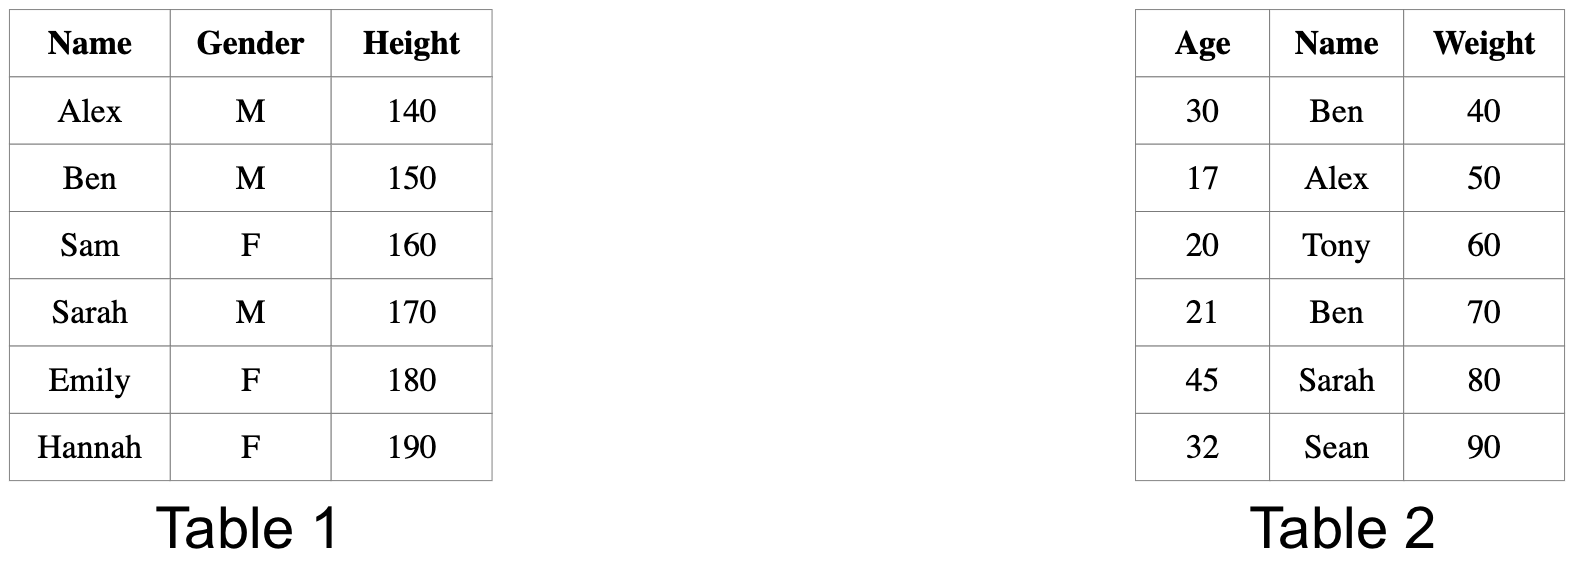
\includegraphics[scale = 0.25]{Masters-Thesis/img/datoy1.png}
    \caption{Toy data set}
    \label{fig:datoy1}
\end{figure}


\section{Linking key columns}

The problem we are trying to solve here is that we want to join the two tables together, to do this we will need to use the key column which is explained above. It gives us information on how the rows from the two tables are joined together. Without the key columns there will be no ways to define what rows belong together. In this section we will be discussing how to draw attention of the user to the key columns and their role. 

Initially, we want the user to focus on the key columns. We do this by first fading out the non-key columns. We use this fading strategy often when we want the user to focus on particular elements at that moment. Second, we show a line linking the key column from both tables. Third, we display a set of words stating which columns we are joining by.


\begin{figure}[H]
    % \centering
    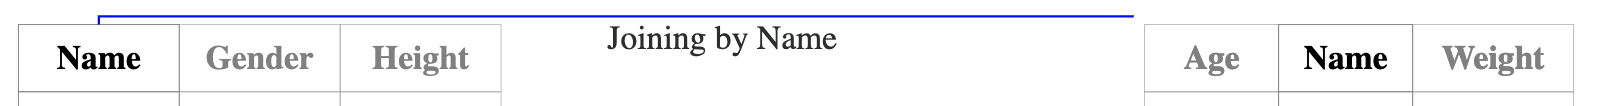
\includegraphics[scale = 0.25]{Masters-Thesis/img/keycol1.png}
    \caption{Key column step 1}
    \label{fig:keycol1}
\end{figure}

Forth, we flash the key column headers on both tables to further focus attention on the key columns.

\begin{figure}[H]
    % \centering
    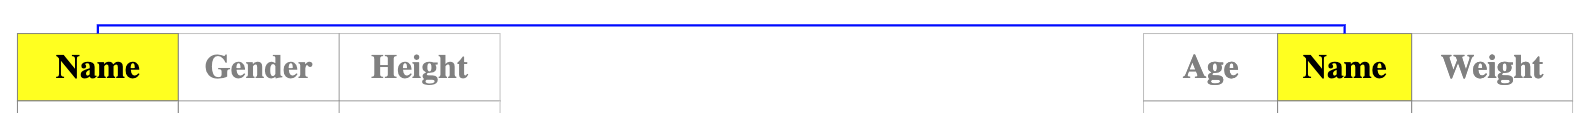
\includegraphics[scale = 0.25]{Masters-Thesis/img/keycol2.png}
    \caption{Key column step 2}
    \label{fig:keycol2}
\end{figure}

Then we need to show the users the structure of the joined table, to do this, we move all column headers except for the key from Table 2 to Table 1, this create new columns/variables in Table 1. After those elements have been moved over, the user can then see the basic structure of the resulted joined table because the rows below the new columns will be empty as shown in Fig.~\ref{fig:keycol3}. The next step is to fill in the empty parts of the rows.

\begin{figure}[H]
    % \centering
    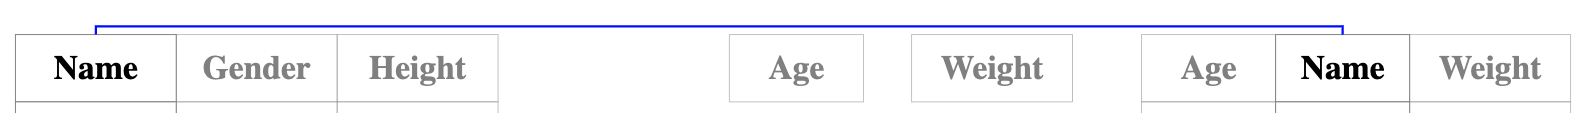
\includegraphics[scale = 0.25]{Masters-Thesis/img/keycol3.png}
    \caption{Key column step 3}
    \label{fig:keycol3}
\end{figure}

Once this structure has been emphasised the faded-out elements then revert back to normal. The original columns in table 1 will remain bold-ed whereas the new columns are not, this is to remind the user which columns are being joined on.

\begin{figure}[H]
    % \centering
    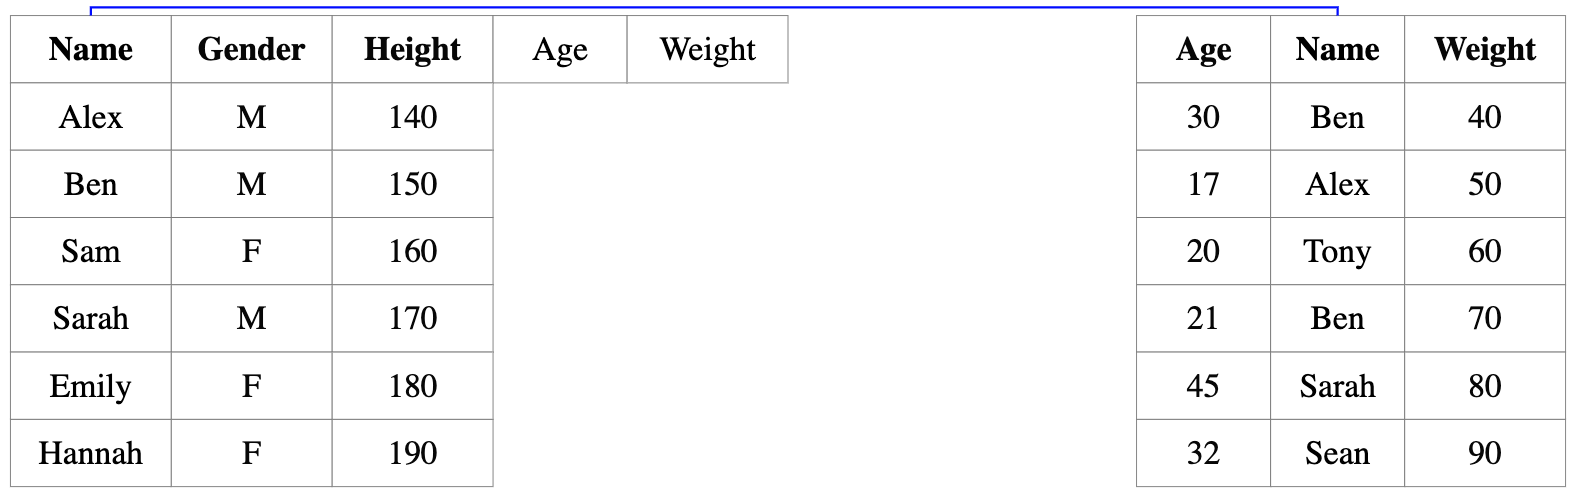
\includegraphics[scale = 0.25]{Masters-Thesis/img/keycol4.png}
    \caption{Key column step 4}
    \label{fig:keycol4}
\end{figure}

Next we will talk about how to fill in the empty rows, the joining process.

\section{Joining process}
In all joins, as part of joining information on rows from the two tables that belong together, elements from the key column in Table 1 will try find a match in the key column of table 2 sequentially until the end of Table 1.

\subsection{The case of a Single match}
Here, Alex is in the first row of Table 1. The join then tries to find Alex in table 2. 
In this scenario, there are matched elements from both key columns, since we have Alex in both tables, this means that these rows can be joined together. 

First, to draw attention to why and how these rows are being joined together, if there is a match on both tables, both matched elements from both key columns flash, and a line then links them together (Fig.~\ref{fig:single1}). 

\begin{figure}[H]
    % \centering
    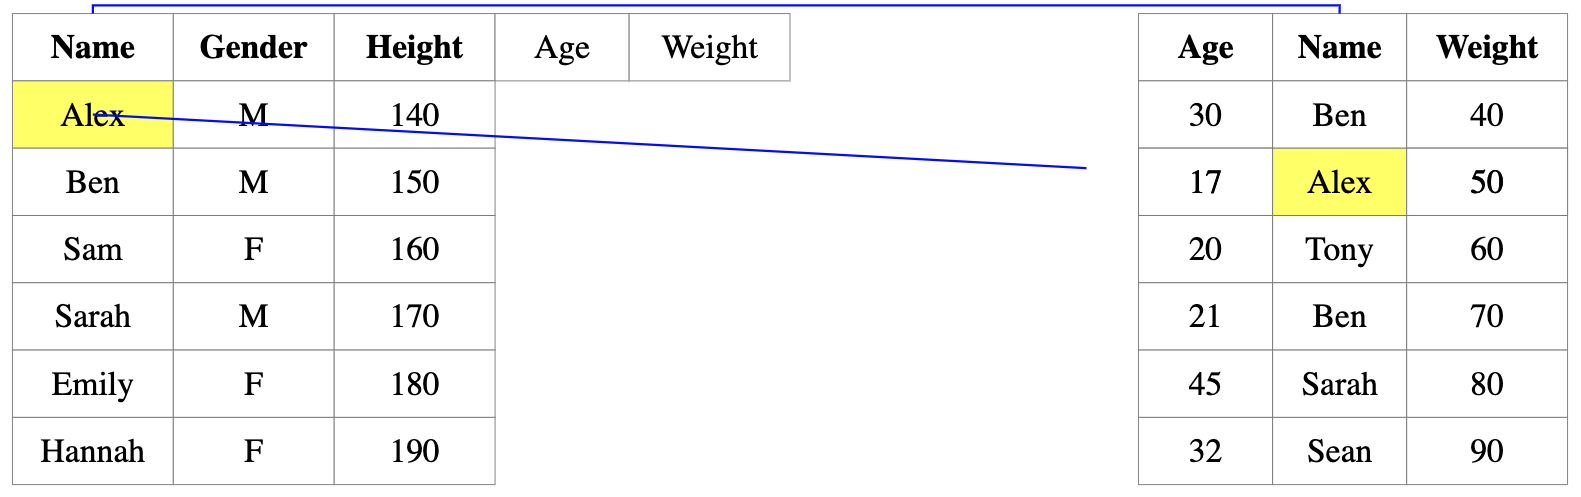
\includegraphics[scale = 0.25]{Masters-Thesis/img/single1.png}
    \caption{Single match step 1}
    \label{fig:single1}
\end{figure}

Second, a message will show explaining that we are currently “Matching Alex” (Fig.~\ref{fig:single2}).

\begin{figure}[H]
    % \centering
    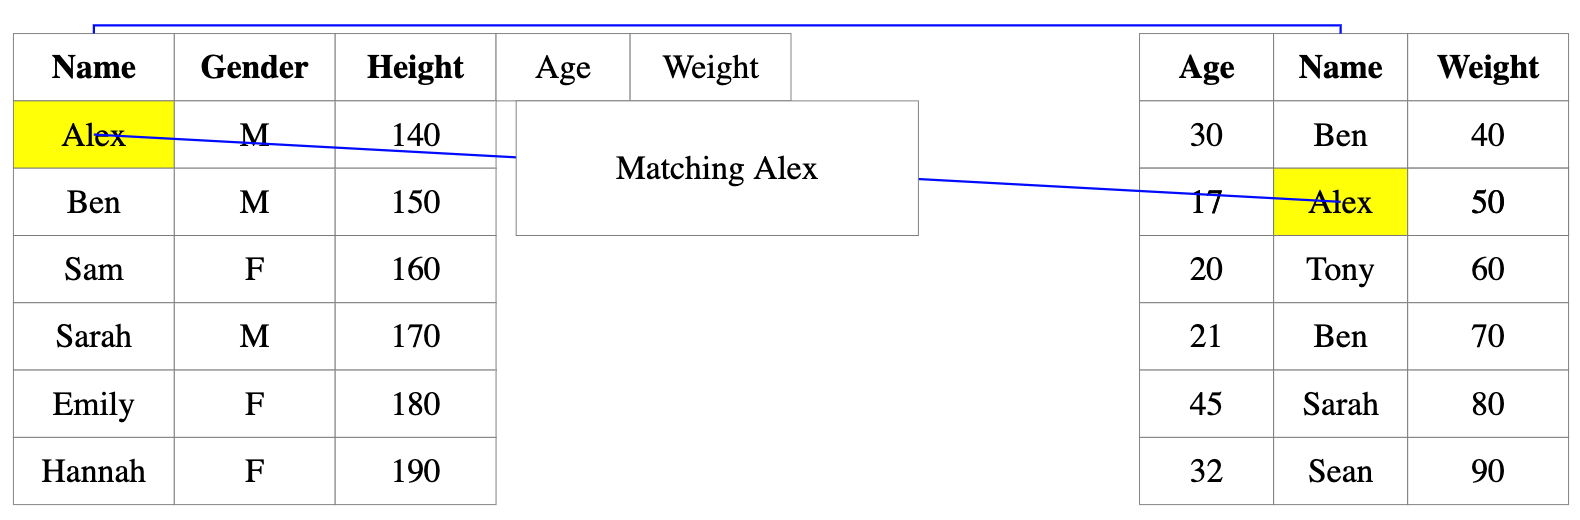
\includegraphics[scale = 0.25]{Masters-Thesis/img/single2.png}
    \caption{Single match step 2}
    \label{fig:single2}
\end{figure}

Then the actual join will perform, all elements except the key from the matched row in table 2 will move across to table 1 (Fig.~\ref{fig:single3} caught mid-move).

\begin{figure}[H]
    % \centering
    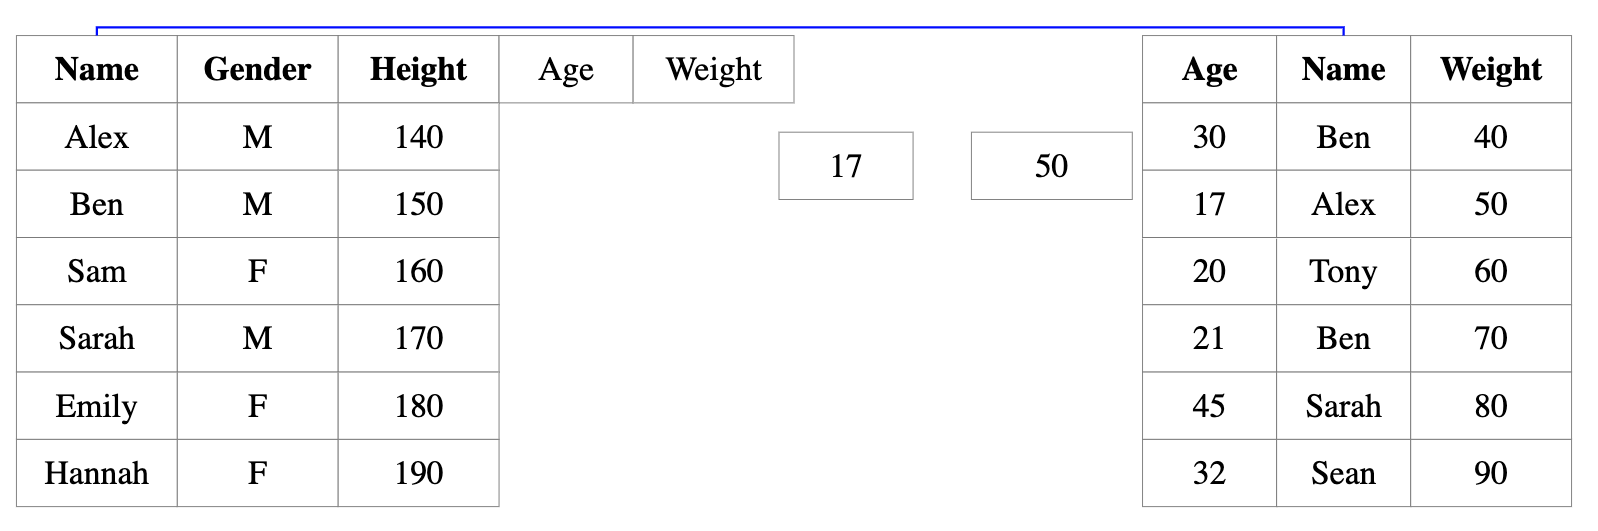
\includegraphics[scale = 0.25]{Masters-Thesis/img/single3.png}
    \caption{Single match step 3}
    \label{fig:single3}
\end{figure}

Lastly, to show the user that the information on Alex in Table 2 has now been used, and we don’t need to play attention to that particular row anymore, we fade out that particular row in Table 2 (Fig.~\ref{fig:single4}).

\begin{figure}[H]
    % \centering
    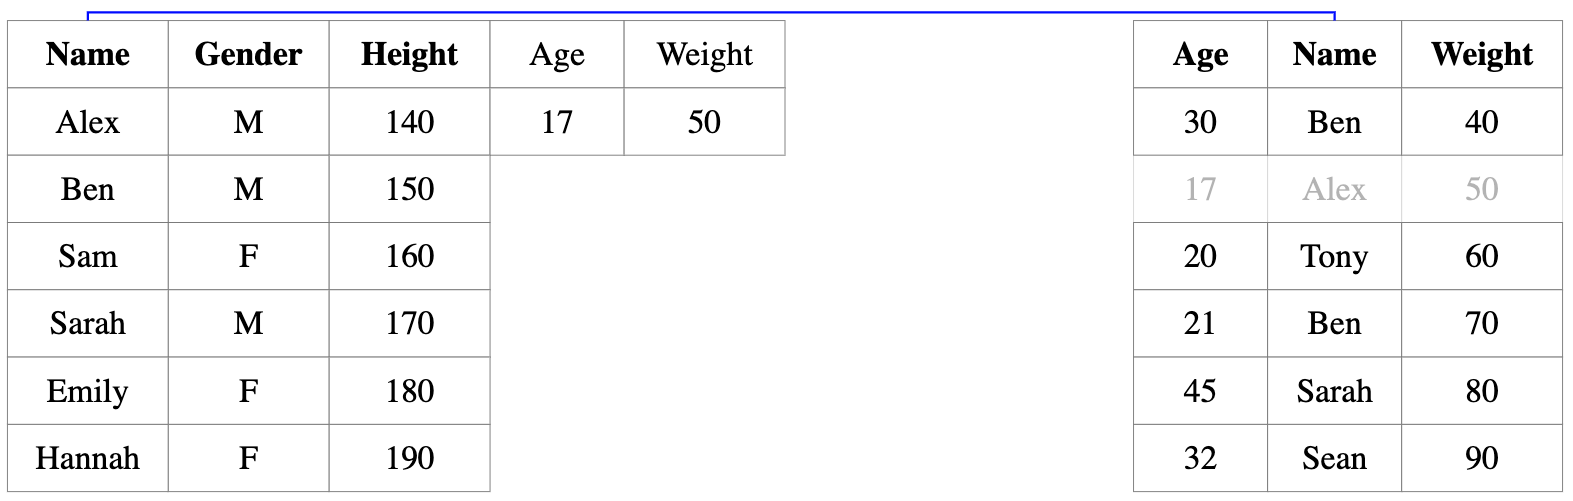
\includegraphics[scale = 0.25]{Masters-Thesis/img/single4.png}
    \caption{Single match step 4}
    \label{fig:single4}
\end{figure}

We then move on to Ben, then Sam and so on down Table 1.

\subsection{The case of Multiple matches}
This occurs when a row in Table 1 matches multiple rows in Table 2.

Like the single match scenario, to allow the users focus on the rows that are being matched, their elements will flash, but this time we will see that there is more than one line matching the rows because there is more than one match found. \\

To reinforce the user that there are more than one rows that match and we want to draw attention to some different behaviour, we show “2 matches found for Ben” (Fig.~\ref{fig:multiple1}).

\begin{figure}[H]
    % \centering
    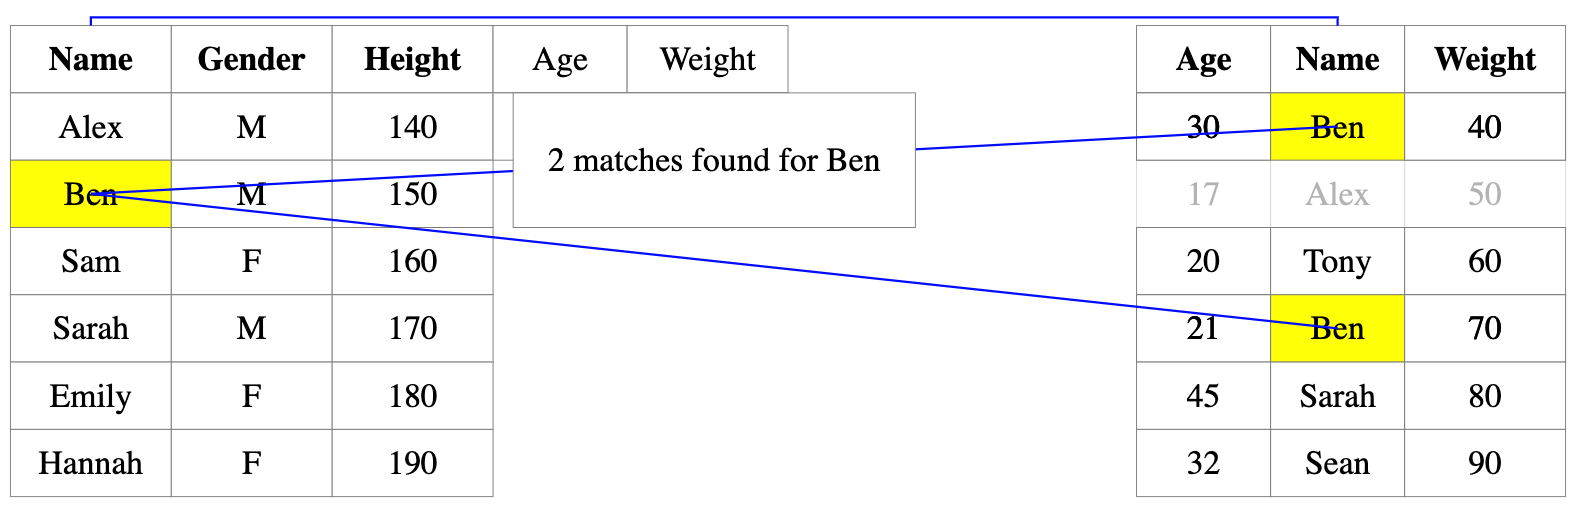
\includegraphics[scale = 0.25]{Masters-Thesis/img/multiple1.png}
    \caption{Multiple matches step 1}
    \label{fig:multiple1}
\end{figure}

We want to move two rows of data from Table 2 across to Table 1 This causes a problem, because there is only one row in Table 1 which matched Table 2.  \\

To solve this we need to compensate by adding an extra row to Table 1, duplicating the matched row from Table 1 (Fig.~\ref{fig:multiple2}). Fig.~\ref{fig:multiple2} also shows the two "Ben" rows from Table 2 in the process of being moved across.  

\begin{figure}[H]
    % \centering
    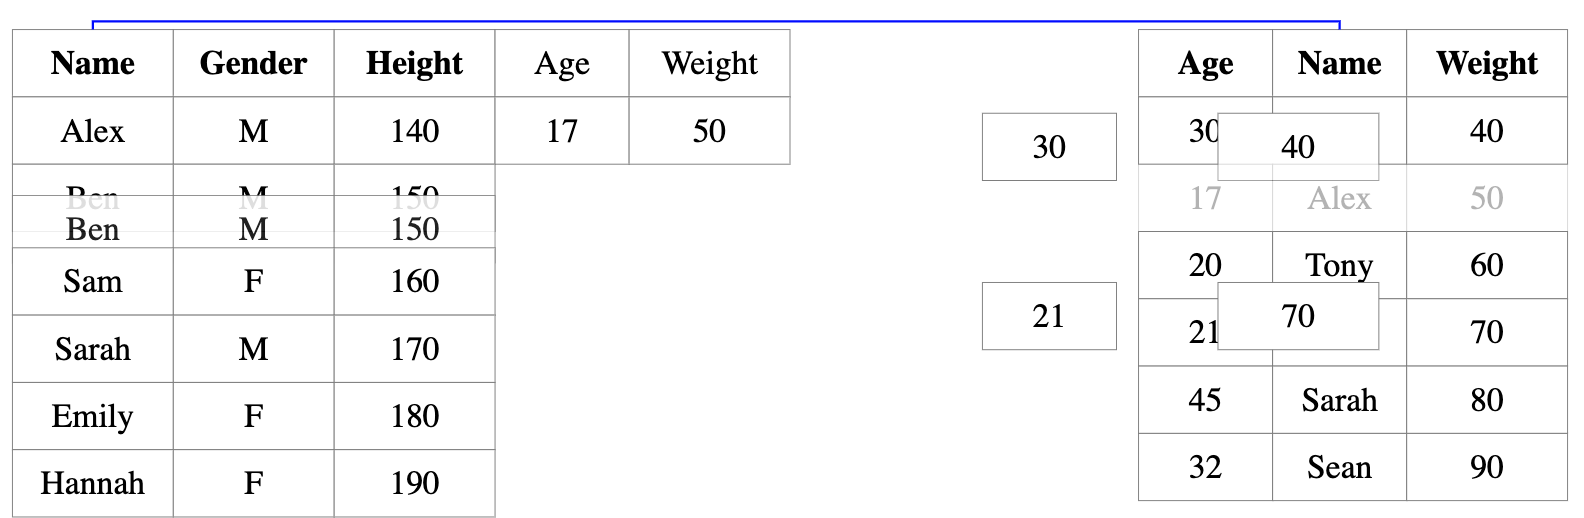
\includegraphics[scale = 0.25]{Masters-Thesis/img/multiple2.png}
    \caption{Multiple matches step 2}
    \label{fig:multiple2}
\end{figure}

\subsection{The case of No match}
What happens when we get to a row in Table 1 with no match in Table 2? Here we don’t have Sam in the key column of Table 2 (Fig.~\ref{fig:nomatch1}). \\

To show this we first flash the row that is currently looking for a match to show the user that this row is currently looking for a match. 
Second, we animate a line to move from that particular element towards Table 2 to show that the join is in the process of looking for a match. 
Third, we stop the line from moving towards table 2 and a pop up question mark. 
Lastly, we pop up a message telling the user that there were no match found. \\

Actions for the no-matches found . case differs between different type of join, as discussed in in paragraphs that follow.

\begin{figure}[H]
    % \centering
    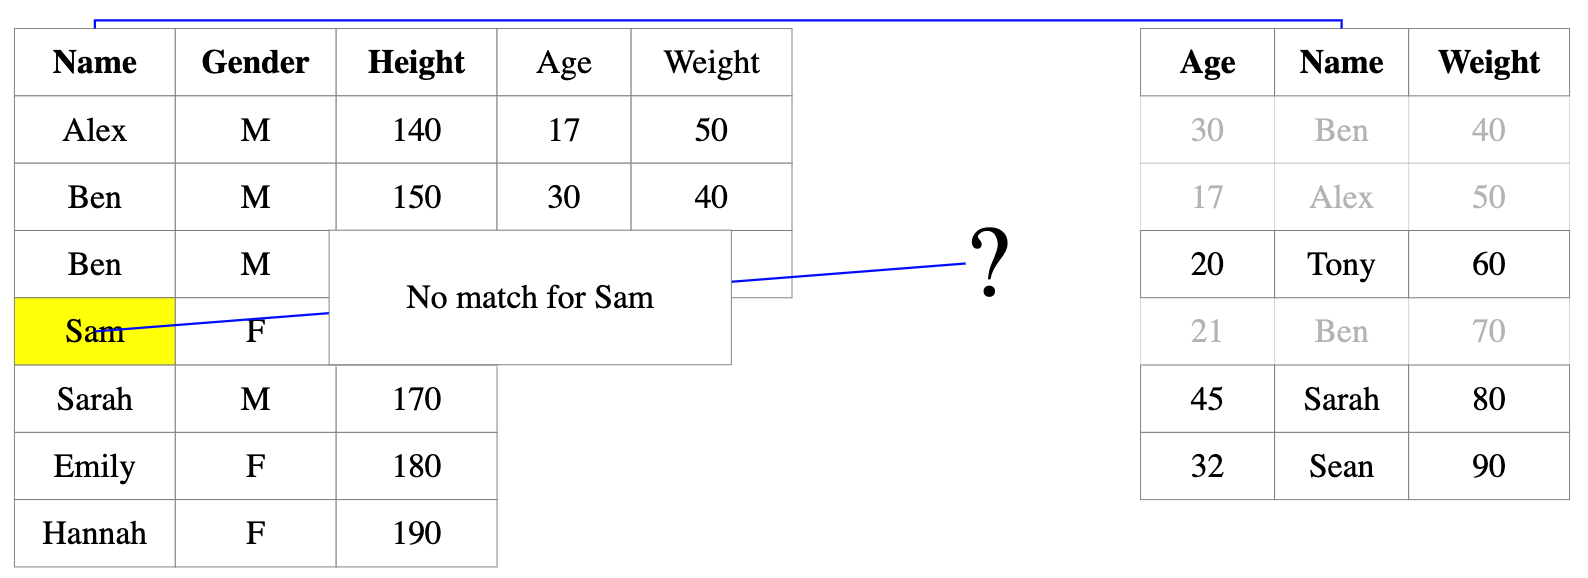
\includegraphics[scale = 0.25]{Masters-Thesis/img/nomatch1.png}
    \caption{No match}
    \label{fig:nomatch1}
\end{figure}

\section{Left/Right Join}
We only show a left join because we get the same resulting join as a right join by left-joining in the reverse order. \textit{Left/Right joins} are also known as \textit{left/right outer joins}.

\begin{figure}[H]
    \centering
    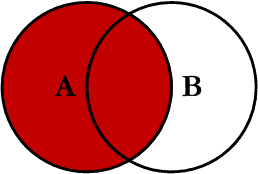
\includegraphics[scale = 0.5]{Masters-Thesis/img/vennleft.png}
    \caption{Venn diagram of Left Join}
    \label{fig:vennleft}
\end{figure}

The definition of a left join is that it returns  data relating to all rows from Table 1, and the matching rows from Table 2. 

For a left join, when there are no matches found, the row in Table 1 is still kept, but there is no information on Table 2 variables for this unit. Therefore those values from the new Table 2 variables are missing (NA).
To show this we then replace the missing values with NA which is the term for missing value in R. Since Sam was not found in Table 2, we fill their Age and Weight columns with NA.

\begin{figure}[H]
    % \centering
    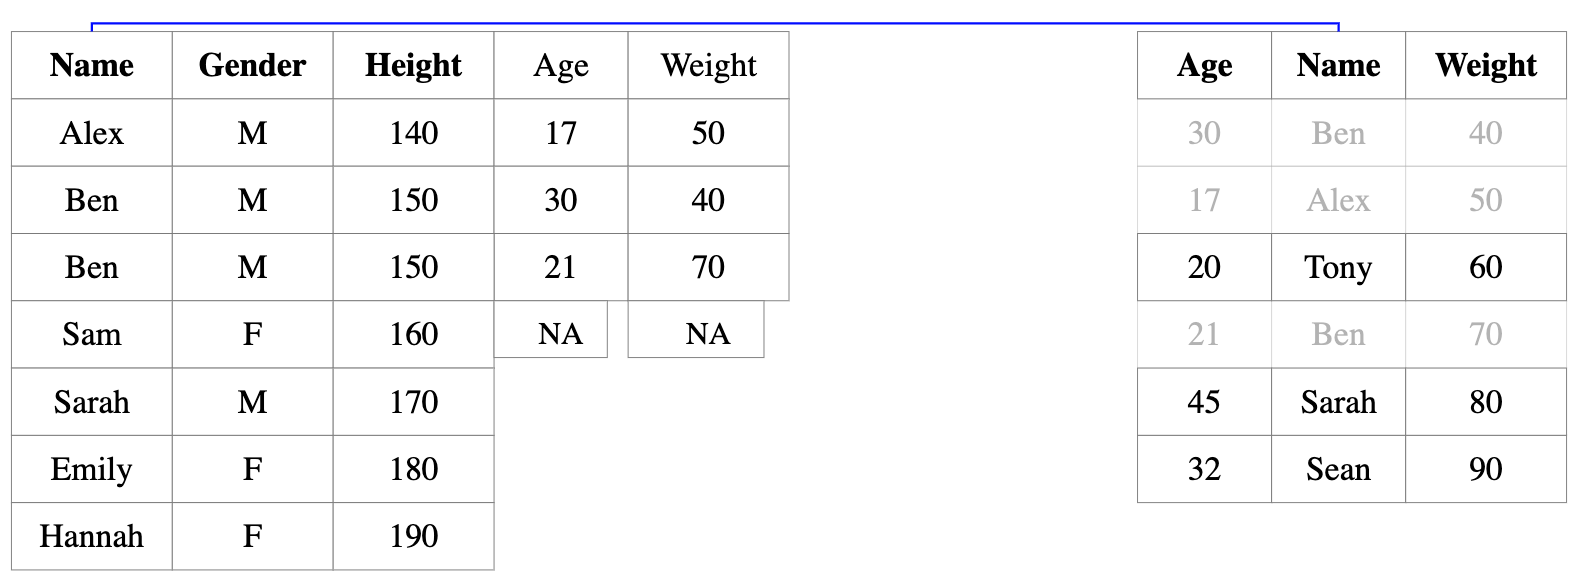
\includegraphics[scale = 0.25]{Masters-Thesis/img/left1.png}
    \caption{Left Join step 1}
    \label{fig:left1}
\end{figure}

After the last row in Table 1 finishes matching, the join is complete. To show the user which rows were used, we can see that some rows are faded out in Table 2. By this strategy, all the usable information in Table 2 has already been used. What is left in Table 2 corresponds to units that are not to be used because they do not appear in Table 1 (see Fig.~\ref{fig:left2}).

\begin{figure}[H]
    \centering
    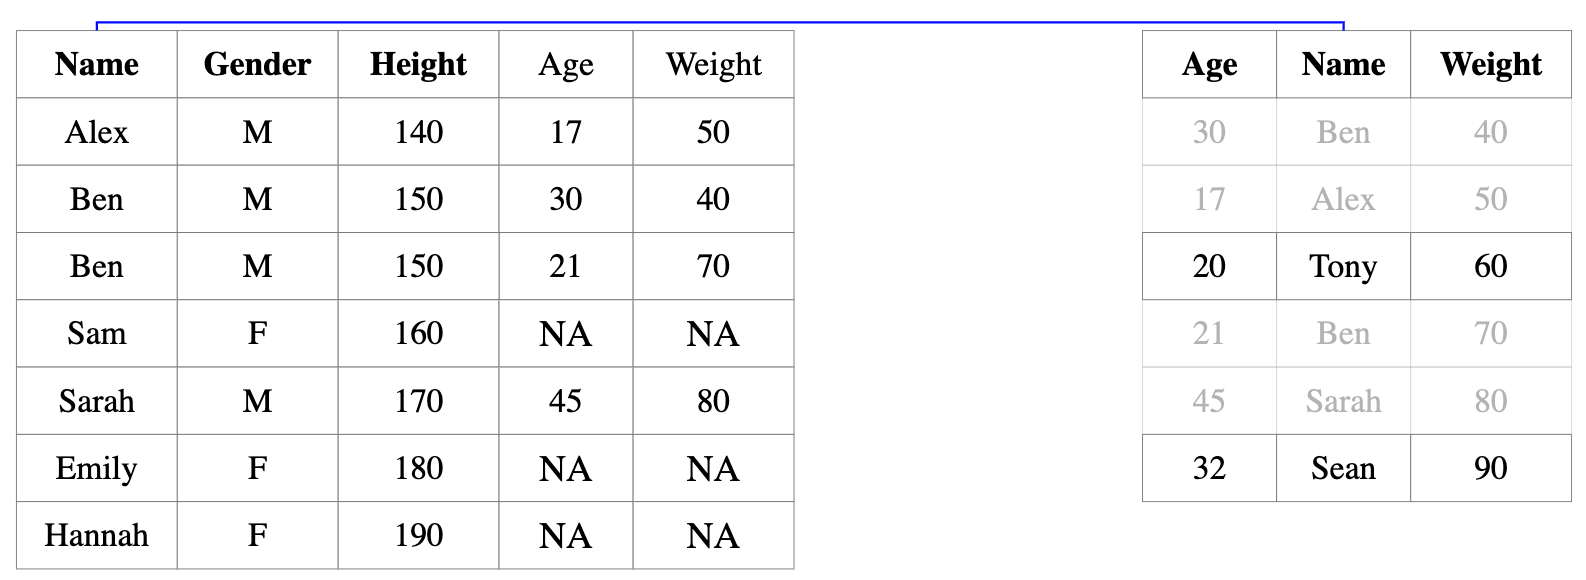
\includegraphics[scale = 0.25]{Masters-Thesis/img/left2.png}
    \caption{Left Join step 2}
    \label{fig:left2}
\end{figure}

To show the user that the join is complete, Table 2 fade away because it is not needed anymore, and Table 1 is moved to the middle so the user can see clearly the resulted joined Table (Fig.~\ref{fig:left3}). 

\begin{figure}[H]
    \centering
    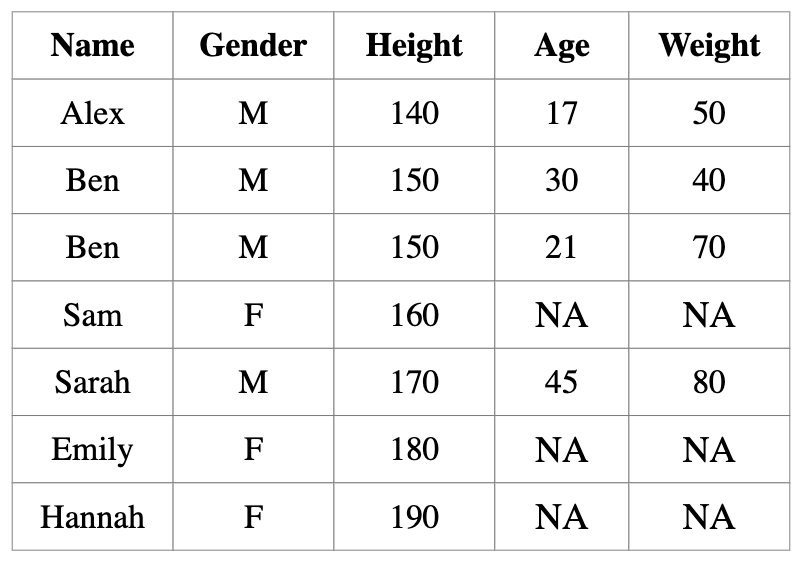
\includegraphics[scale = 0.25]{Masters-Thesis/img/left3.png}
    \caption{Left Join step 3}
    \label{fig:left3}
\end{figure}

\section{Inner Join}
The main idea of a inner join is to combine information on only those units that appear in \textbf{both} Table 1 and Table 2. That is why they are typically represented by a intersection in a Venn diagram. 

\begin{figure}[H]
    \centering
    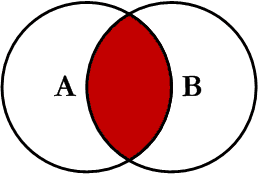
\includegraphics[scale = 0.5]{Masters-Thesis/img/venninner.png}
    \caption{Venn diagram of Inner Join}
    \label{fig:venninner}
\end{figure}

The definition of a inner join is it returns rows that have matching key column values in both tables. This is similar to the left join explained above but since it only returns rows that have matching key columns in both tables. When no match is found for a Table 1 row in Table 2, we remove that row in Table 1 instead of filling in NA for the missing values (Fig.~\ref{fig:inner1}, \ref{fig:inner2}). 

\begin{figure}[H]
    % \centering
    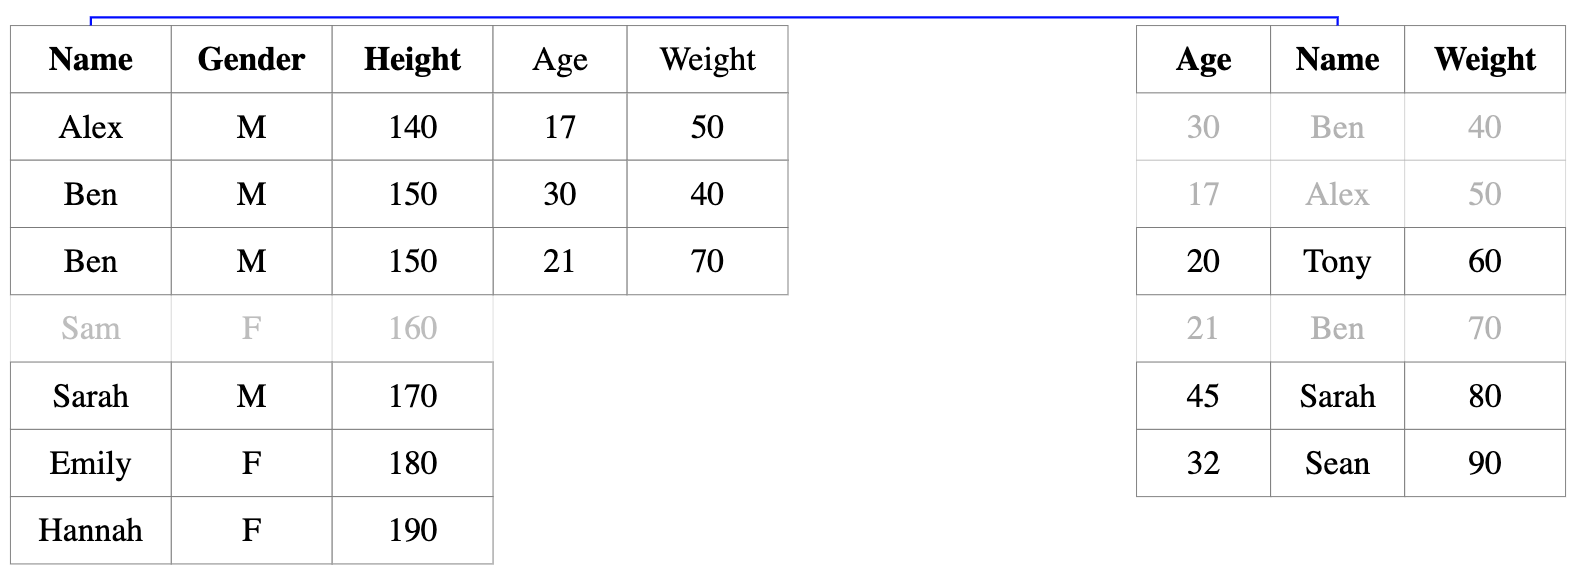
\includegraphics[scale = 0.25]{Masters-Thesis/img/inner1.png}
    \caption{Inner Join step 1}
    \label{fig:inner1}
\end{figure}

At the end of the join, the user will be able to see which rows did not find a match, from the gaps between rows in Table 1. This is to remind the user that there are rows that were removed because there were no matches for them.

\begin{figure}[H]
    % \centering
    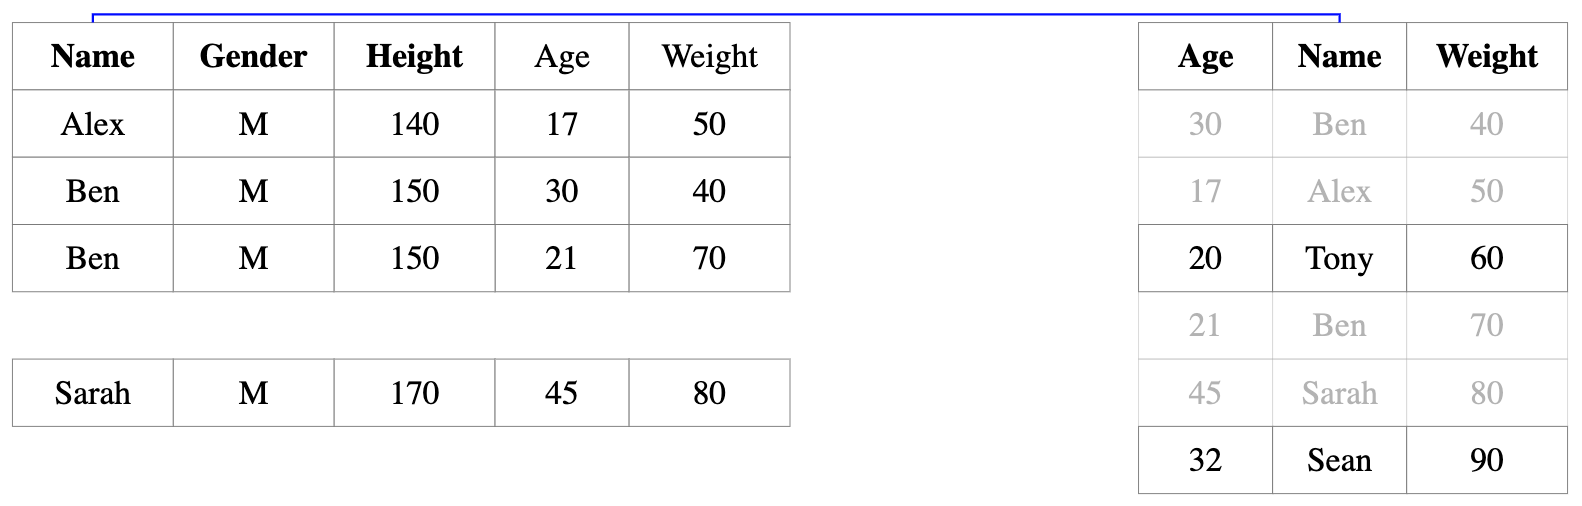
\includegraphics[scale = 0.25]{Masters-Thesis/img/inner2.png}
    \caption{Inner Join step 2}
    \label{fig:inner2}
\end{figure}

Similar to left join, to show that the join is finished, Table 2 will be removed and the resulted joined table will be centred. The only difference is that all the rows will be pushed together to fill in the gaps produced by the removed rows (Fig.~\ref{fig:inner3}).

\begin{figure}[H]
    \centering
    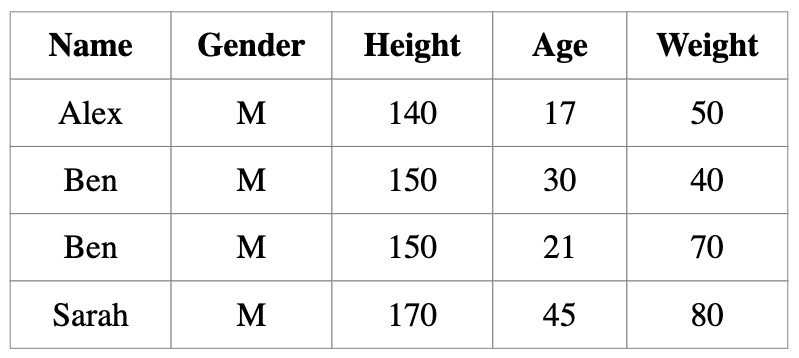
\includegraphics[scale = 0.3]{Masters-Thesis/img/inner3.png}
    \caption{Inner Join step 3}
    \label{fig:inner3}
\end{figure}

\section{Full Join}
The full join is also known as a complete join. The main idea of a full join is to combine information on all units that appear in either Table 1 or Table 2 or both. That is why they are often represented by a union in a Venn diagram.

\begin{figure}[H]
    \centering
    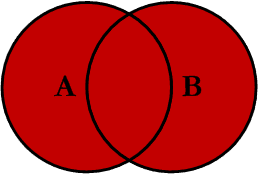
\includegraphics[scale = 0.5]{Masters-Thesis/img/vennfull.png}
    \caption{Venn diagram of Full Join}
    \label{fig:vennfull}
\end{figure}

The definition of a full join is it returns all rows relating to key column values found in Table 1, Table 2 or both. For a complete join, the first step of the joining process is the same as a left join. The difference is that when the matching process is done, the left join is complete, whereas the full join now will move the unmatched rows from the Table 2 to Table 1. \\

The problem here is that we will need to move the remaining unmatched rows from Table 2 that have not been used, these are rows in Table 2 that are not faded out (because they have already been used). 

First, to catch the users attention, we flash the elements from the key column in the unmatched rows in Table 2.
Second, we animate a line and a question mark showing the user that they are the unmatched rows and there is no where for them to go (Fig.~\ref{fig:full1}).

\begin{figure}[H]
    % \centering
    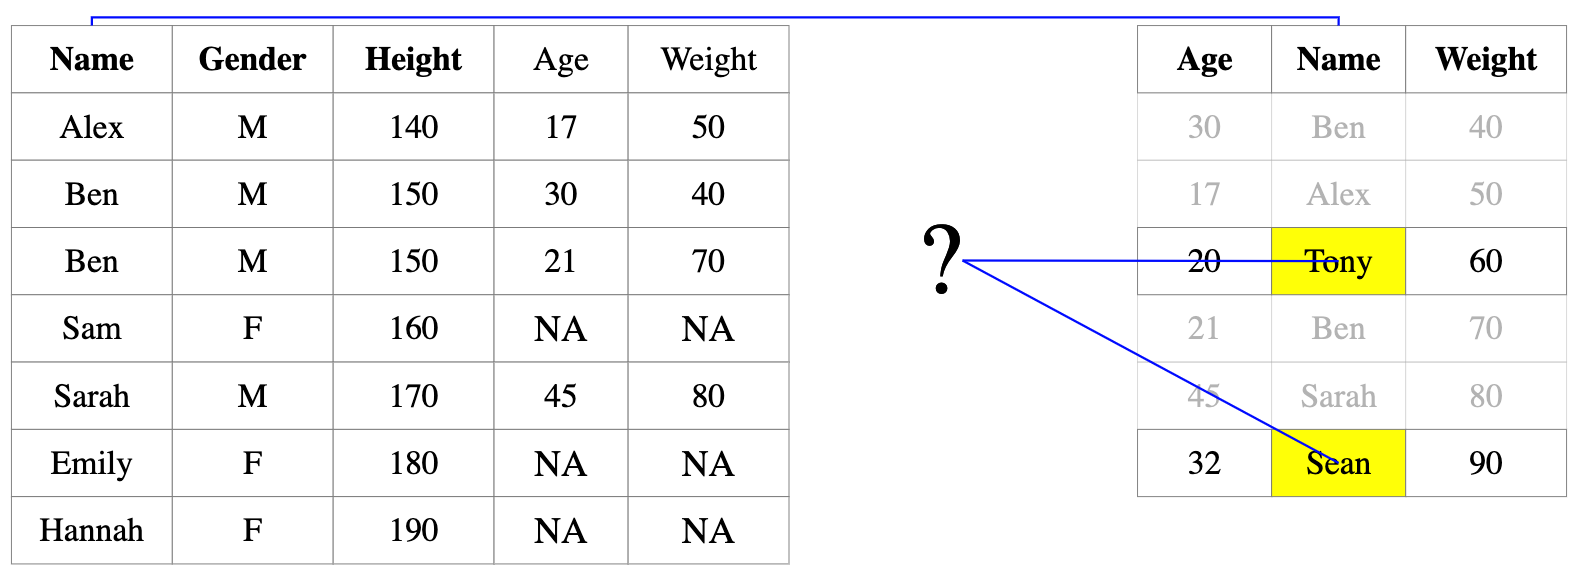
\includegraphics[scale = 0.25]{Masters-Thesis/img/full1.png}
    \caption{Full Join step 1}
    \label{fig:full1}
\end{figure}

\newpage
Third, we show a message indicating that (Fig.~\ref{fig:full2}). Then we move the unused rows across to Table 1, this is to remind the user what the next step is.

\begin{figure}[H]
    % \centering
    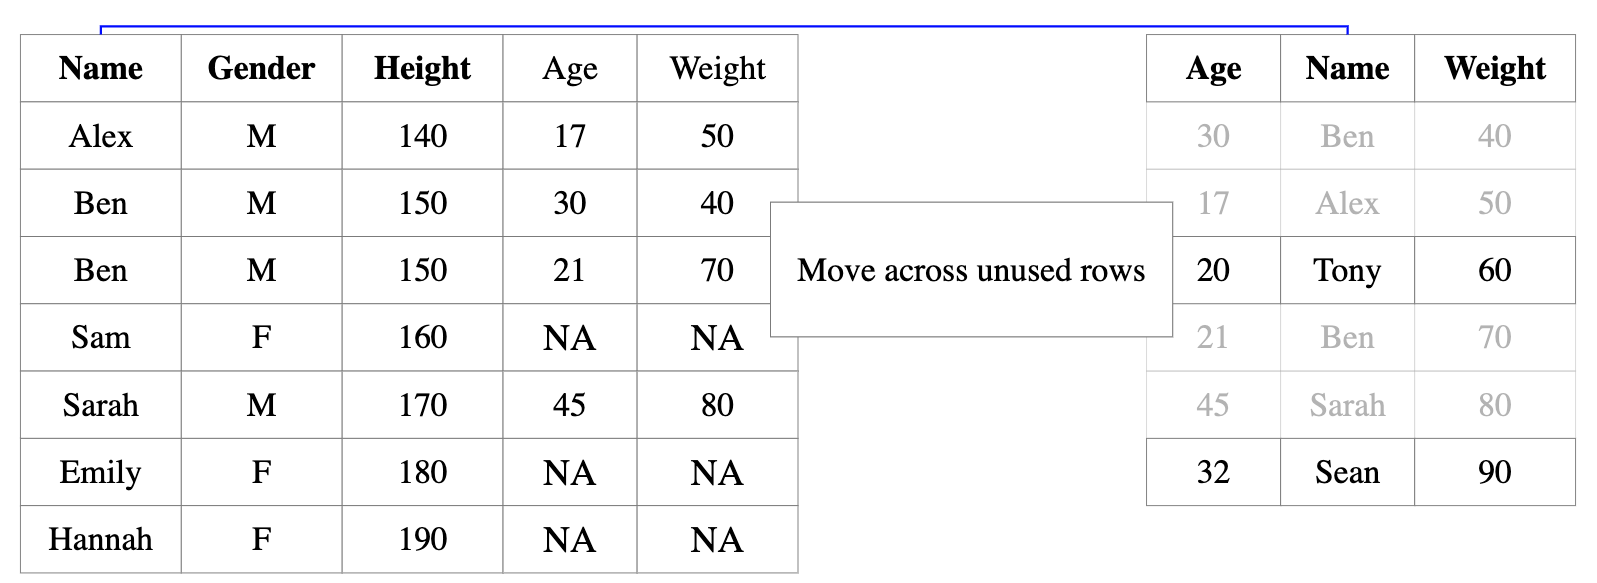
\includegraphics[scale = 0.25]{Masters-Thesis/img/full2.png}
    \caption{Full Join step 2}
    \label{fig:full2}
\end{figure}

Fourth, we move the unmatched rows from Table 2 across to Table 1, to their corresponding column in row order (Fig.~\ref{fig:full3}).

\begin{figure}[H]
    % \centering
    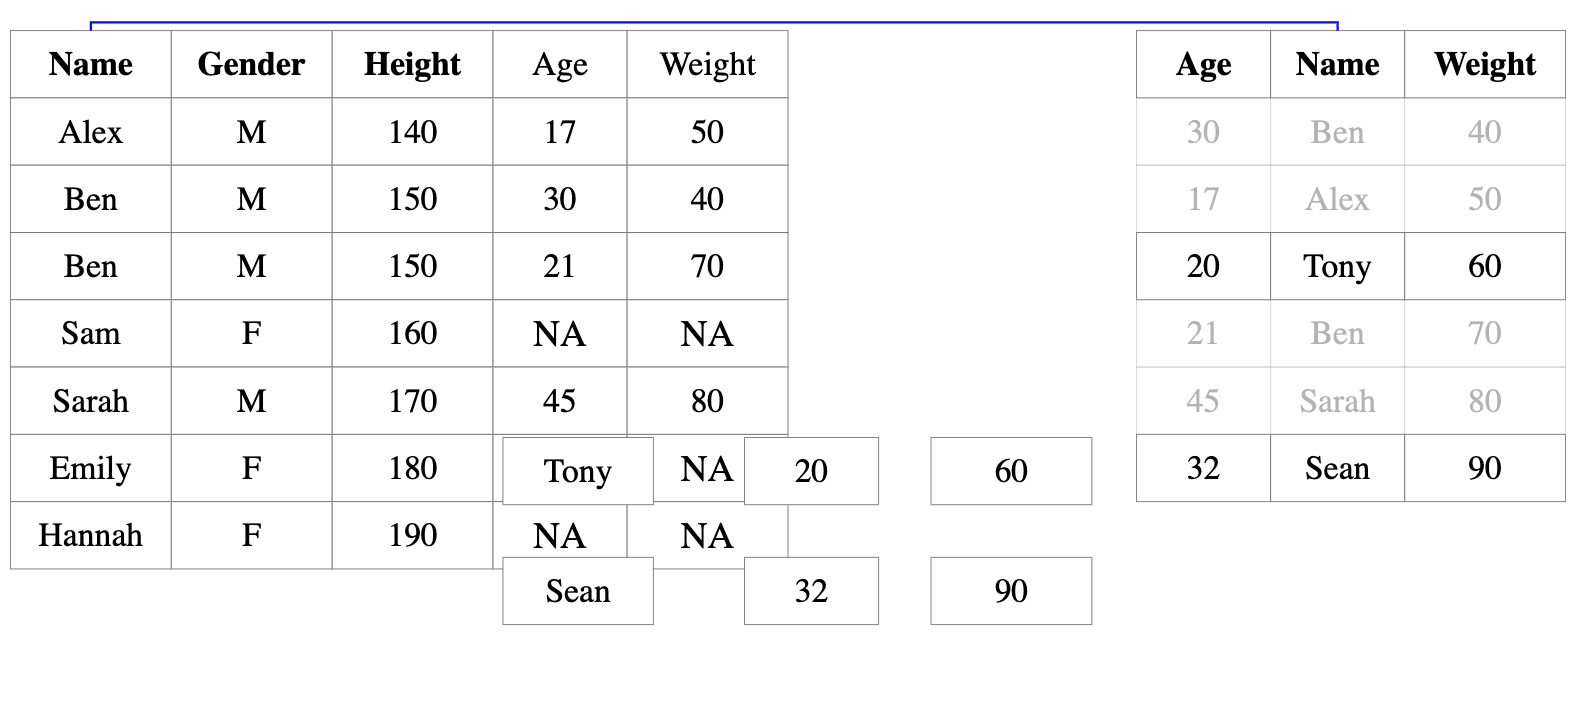
\includegraphics[scale = 0.25]{Masters-Thesis/img/full3.png}
    \caption{Full Join step 3}
    \label{fig:full3}
\end{figure}

\newpage

After the rows are moved across, the cells corresponding to the Table 1 variables will be empty. To complete the join we will need to fill these with NAs to indicate that these are missing values. \\

Therefore, fifth, to convey this idea, we flash this region in red, question marks will also appear showing the user that this region is missing, and that we do not have any information in these data (Fig.~\ref{fig:full4}). 

\begin{figure}[H]
    % \centering
    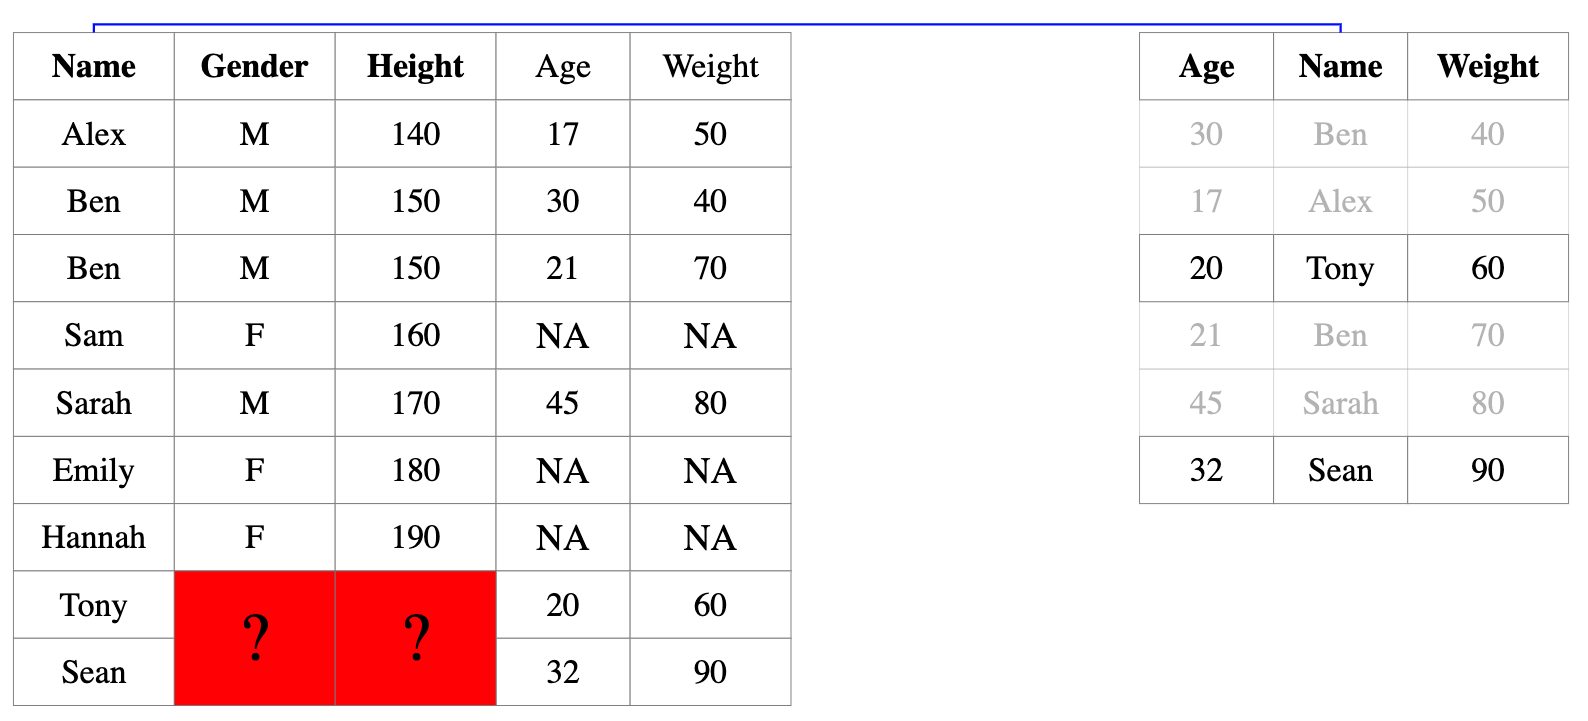
\includegraphics[scale = 0.25]{Masters-Thesis/img/full4.png}
    \caption{Full Join step 4}
    \label{fig:full4}
\end{figure}

Then we replace these empty elements with NA, similar to what we did with a left join (Fig.~\ref{fig:full5}). 

\begin{figure}[H]
    % \centering
    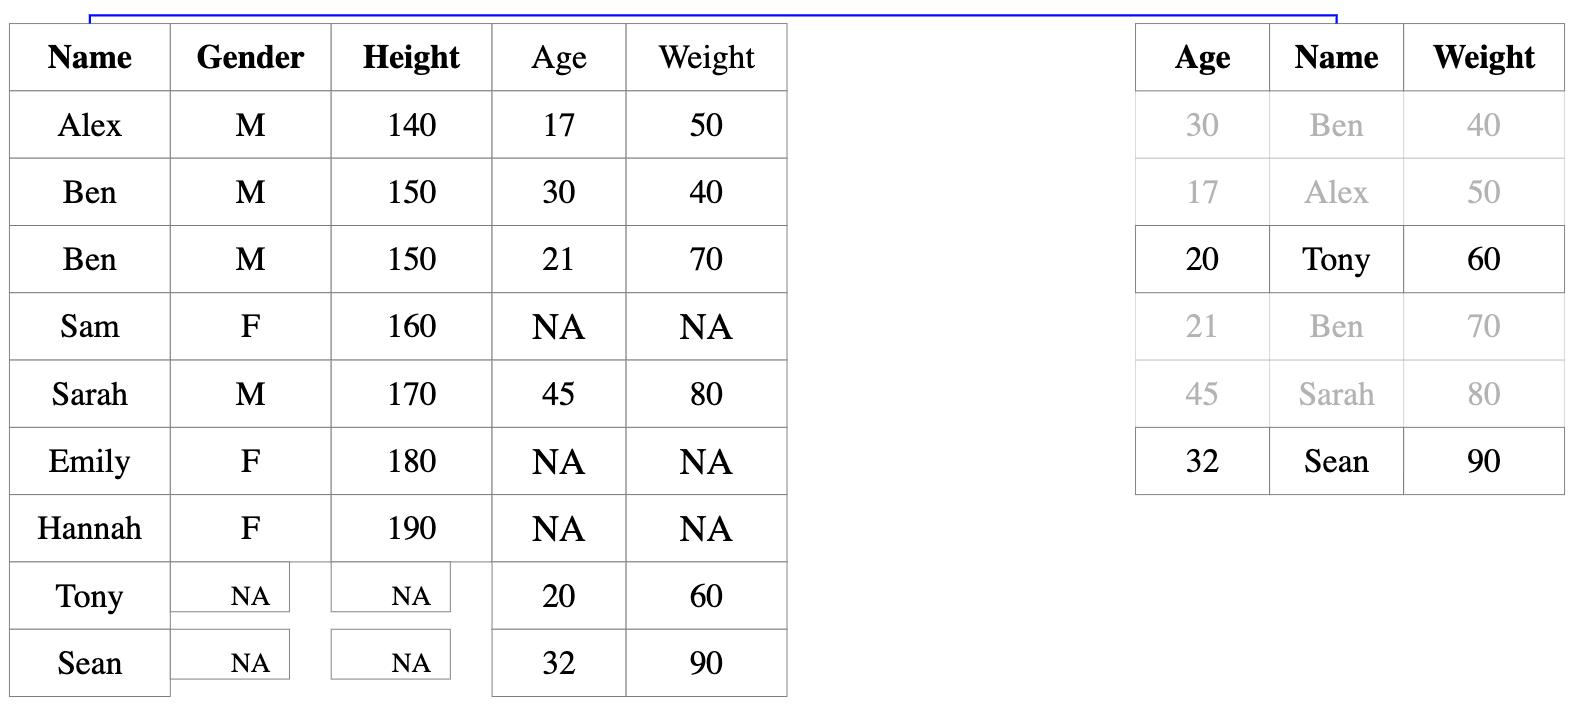
\includegraphics[scale = 0.25]{Masters-Thesis/img/full5.png}
    \caption{Full Join step 5}
    \label{fig:full5}
\end{figure}

\newpage

Lastly, at the end of the join, we isolate the resulted joined table to the middle to show the user that this is finished (Fig.~\ref{fig:full6}).

\begin{figure}[H]
    \centering
    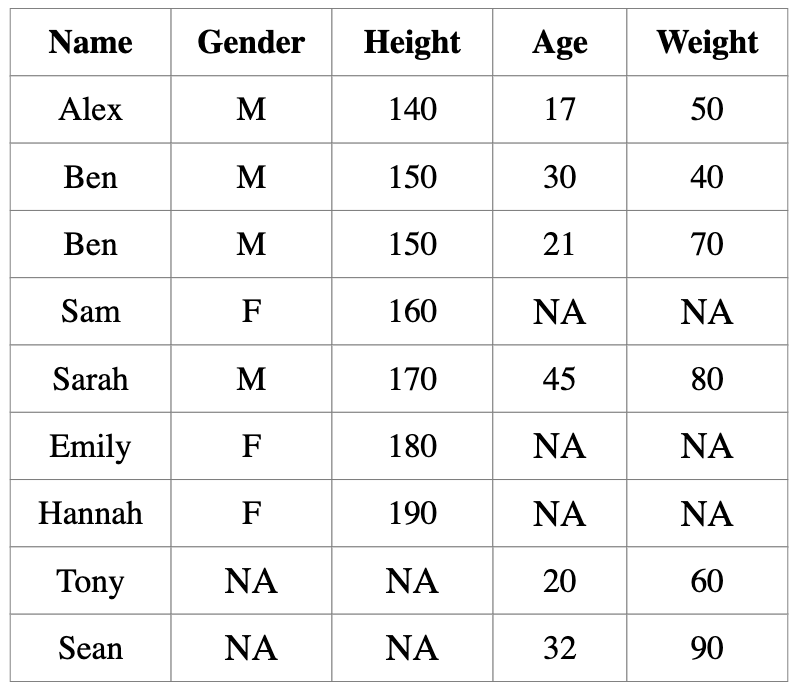
\includegraphics[scale = 0.3]{Masters-Thesis/img/full6.png}
    \caption{Full Join step 6}
    \label{fig:full6}
\end{figure}

%% Chapter Template
%
\chapter{Methodology for Data Reshaping} \label{c4} % Main chapter title

\section{Software Structre}

The software structure for the reshaping module is the same as the joining module, refer to Section~\ref{s2.ss} and Fig.~\ref{fig:softflow}.

\section{\textbf{R}}
In the reshaping module, we still use the \textbf{dplyr} and \textbf{tidyr} package. The difference is that in the joining module, we used \textbf{dplyr} more frequently because it provided us with functions to join data sets together. In the reshaping module, \textbf{tidyr} was used more frequently because it contains functions to reshape data sets. 

The idea is the same, but instead of passing information to \textsf{JavaScript} to perform joining animations, we pass in information to perform reshaping animations. They include,

\begin{itemize}
    \item The dimensions and information of the inputted table.
    \item The dimension and information of the resulted table.
    \item The text of the instructional messages to be displayed.
    \item The name and column number of the key columns.
    \item The name and column number of the values columns. 
    \item The corresponding position of where each cell elements within a table goes (in matrix notation).
\end{itemize}

\section{\textbf{dataAnim}}

The reshaping module brings two new functions to the \textbf{dataAnim} package, the \texttt{spread\_anim} function to generate a long to wide animation and the \textttt{gather\_anim} function generates a wide to long animation. \\

The compulsory arguments include the speed of the animation, the data set to apply transformation on, the name of the key and the name of the value. \texttt{gather\_anim} requires an addition argument \texttt{col}, this indicates the columns we wish to reshape on. Below is the help page for \texttt{spread\_anim} shown in Fig.~\ref{fig:spreadhelp} and \texttt{gather\_anim} shown in Fig.~\ref{fig:gatherhelp}.

\begin{figure}[H]
    \centering
    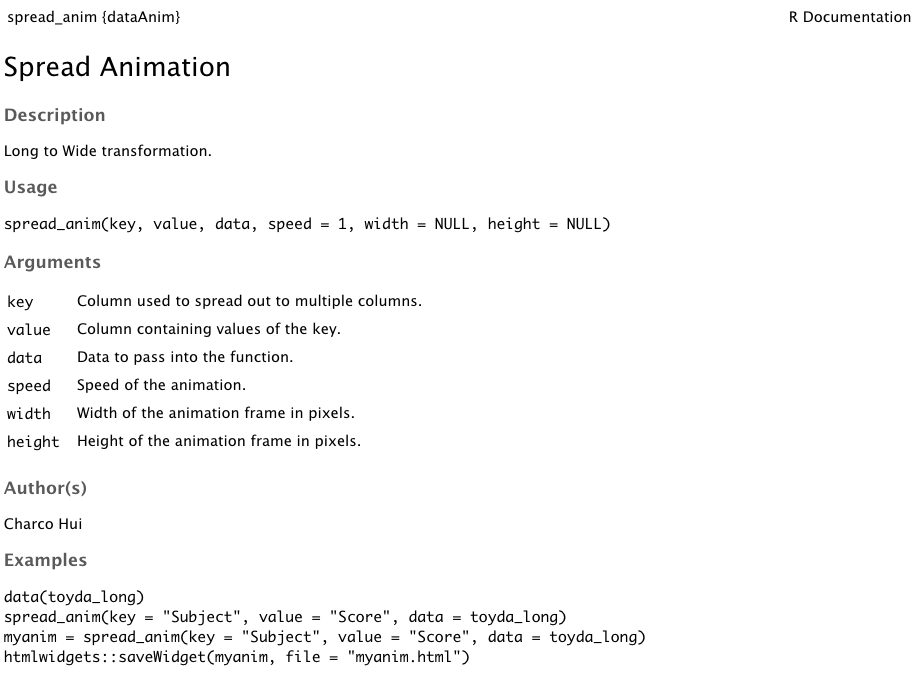
\includegraphics[scale = 0.42]{Masters-Thesis/img/spreadhelp.png}
    \caption{\texttt{spread\_anim} help page}
    \label{fig:spreadhelp}
\end{figure}

\begin{figure}[H]
    \centering
    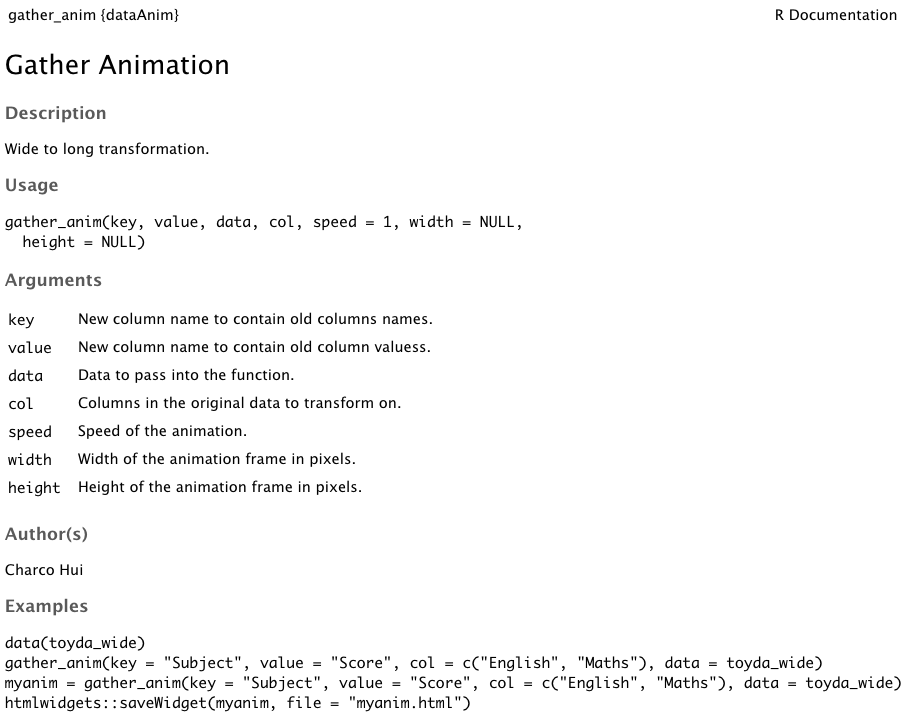
\includegraphics[scale = 0.42]{Masters-Thesis/img/gatherhelp.png}
    \caption{\texttt{gather\_anim} help page}
    \label{fig:gatherhelp}
\end{figure}

\newpage

Discussion of the common arguments:
\begin{itemize}
    \item \texttt{data} is the table to perform reshaping on.
    \item \texttt{speed} allows us to give the user control of the speed of the animation.
    \item \texttt{width} and \texttt{height} are the size of the animation frame in pixels.
\end{itemize}

Discussion of the \texttt{spread\_anim} arguments:
\begin{itemize}
    \item \texttt{key} is the column the user chooses to spread out to multiple columns.
    \item \texttt{value} is the column the that contains the values of the key columns.
\end{itemize}

Discussion of the \texttt{gather\_anim} arguments:

\begin{itemize}
    \item \texttt{key} is the new column name the user wishes to use to contain the old column names.
    \item \texttt{value} is the new column name the user wishes to use to store those values.
    \item \texttt{col} are the columns the user wishes to reshape on.
\end{itemize}
\\

To produce these animation, one method is to use \textbf{Rstudio}. An example of generating a wide to long animation using the \texttt{gather\_anim} in \textbf{Rstudio} is shown in Fig.~\ref{fig:gatherrstudio}.

\begin{figure}[H]
    \centering
    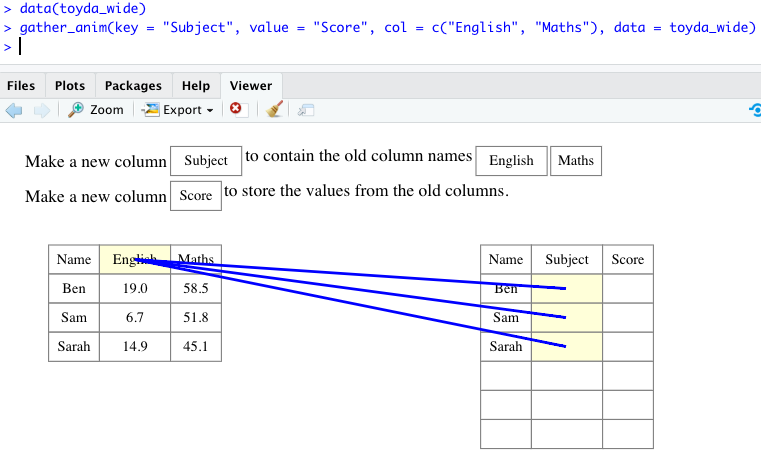
\includegraphics[scale = 0.5]{Masters-Thesis/img/gatherrstudio.png}
    \caption{\texttt{gather\_anim} Example}
    \label{fig:gatherrstudio}
\end{figure}

Another method to generate these animations is to use our \textbf{shiny} interactive dashboard, we will discuss this in Section~\ref{sreshapehtmlwidget}.

\newpage

\section{\textsf{JavaScript} - D3}

In the reshaping module, the use of \textsf{JavaScript} remains the same. However the flow is different. As shown in Fig.~\ref{fig:jsflow2}, the \textsf{JavaScript} program:

\begin{enumerate}
    \item Reads in the instruction from \textsf{R} and passing \textsf{R} objects directly to \textsf{JavaScript} using the \textbf{htmlwidgets} environment. 
    \item Draw the original table given by the user.
    \item Give a brief introduction of the what the animation will be based on.  
    \item Display the structure of the reshaped table. This table will be empty, it is shown to give the user an idea of what the resulted table will look like.
    \item Starts the reshaping animation and display the instructional messages when necessary. 
\end{enumerate}

\begin{figure}[H]
    \centering
    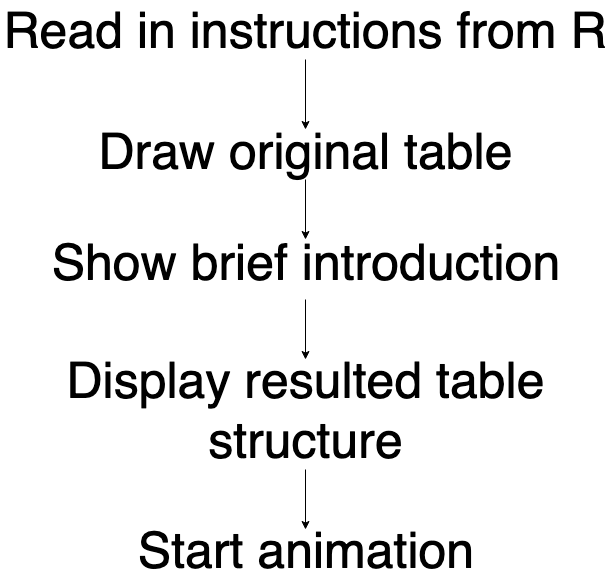
\includegraphics[scale = 0.4]{Masters-Thesis/img/jsflow2.png}
    \caption{\textsf{JavaScript} program flow}
    \label{fig:jsflow2}
\end{figure}


\newpage

\section{\textbf{htmlwidgets} and \textbf{shiny}} \label{sreshapehtmlwidget}
As shown in Fig.~\ref{fig:reshapeshiny}, the \texbf{shiny} interactive dashboard for the reshaping module is different to the joining module. There are three tabs, Tab 1 allow the users to upload their data set in a CSV format, Tab 2 allow users to generate a long to wide animation (Spread) and Tab 3 allow users to generate a wide to long animation (Gather).

\begin{figure}[H]
    \centering
    \begin{tabular}{ccc}
     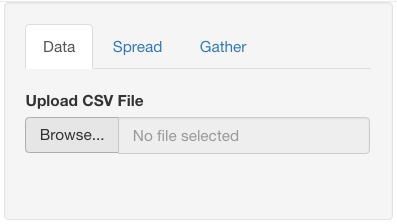
\includegraphics[scale = 0.34]{Masters-Thesis/img/rshinytab1.png} & 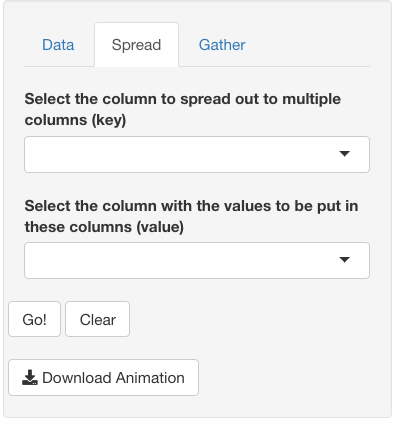
\includegraphics[scale = 0.34]{Masters-Thesis/img/rshinytab2.png} & 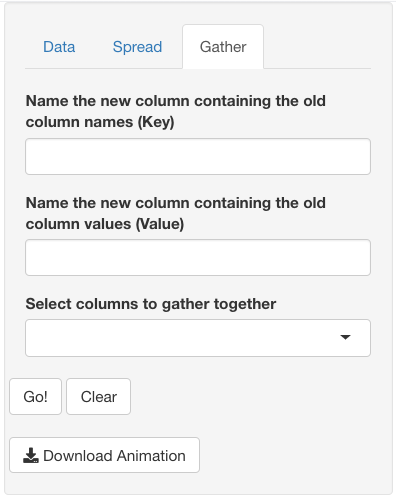
\includegraphics[scale = 0.34]{Masters-Thesis/img/rshinytab3.png} \\
    (a) Tab 1 & (b) Tab 2 & (c) Tab 3 \\[6pt]
    \end{tabular}
    \caption{\textbf{shiny} interactive dashboard (reshape module)}
    \label{fig:reshapeshiny}
\end{figure}

\section{Animation}

In the previous section, some issues with the existing approach of teaching data reshaping were discussed. Some improvements were made to address those issues, with the end goal of making these animations as intuitive as possible. 

The goals of these animations are to:

\begin{itemize}
    \item To show the logic of the data reshaping
    \item Highlight the importance and role of the key and value (columns)
    \item Show the user the relationship between variables in the original table and the resulted table.
    \item Show the underlying process of a wide to long transformation (Spread)
    \item Show the underlying process of a long to wide transformation (Gather)
    \item Show how data are moved between tables
    \item Allow users to download and export the animations.
\end{itemize} 
%% Chapter Template
%
\chapter{Animation for Data Reshaping} \label{c5} % Main chapter title

In this chapter we will discuss how we use animations to expression data reshaping.

\section{Long to Wide (Spread)}

\subsection{Logic of Long to Wide}
The logic of the long to wide transformation in the \texttt{spread} function of \textbf{tidyr} is to use the \texttt{key} and \texttt{value} column. Note that the \texttt{key} does not have the same definition as the key column in data joins. The \texttt{key} here is the column the user wishes to use to spread out to multiple columns and the \texttt{value} is the column that contains their values.

\subsection{Long to Wide Animation}
Before the animation starts, we tell the user that we will be using a old column from the original table given by the user to create new columns in the resulted table by using a message. Here we will use the old column Subject to spread out (create) two columns English and Maths.

We then move elements English and Maths from the original table up to the message because we want the user to know that these are the columns we will be using during the animation (Fig.~\ref{fig:spread1}). We use a table cell like design for this word within the sentence because we want the user to know that we are referring to a certain element in a particular table. We will use this table cell technique often through out the reshaping animation.

\begin{figure}[H]
    % \centering
    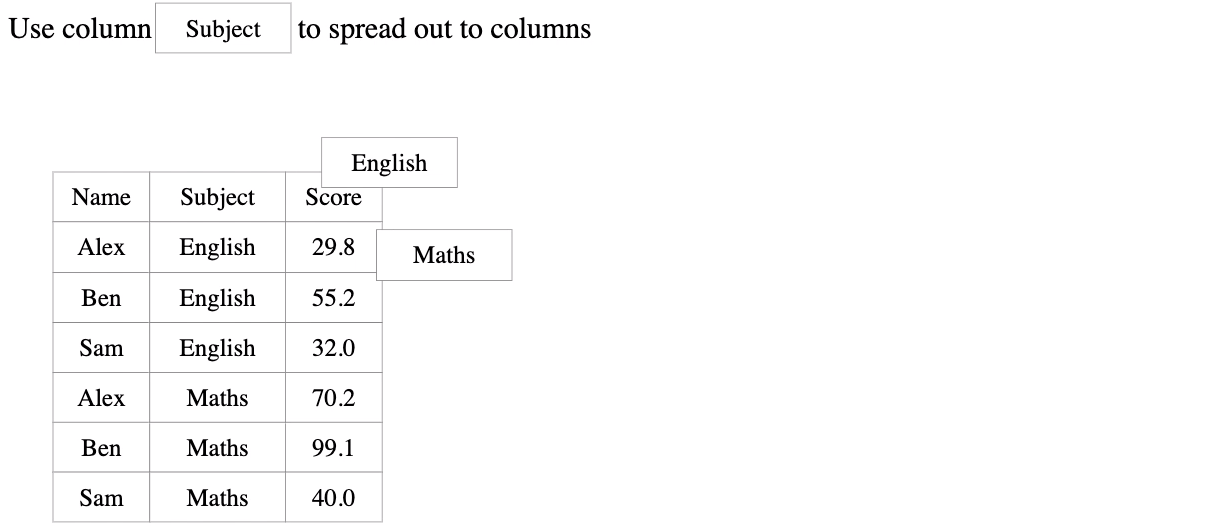
\includegraphics[scale = 0.35]{Masters-Thesis/img/spread1.png}
    \caption{Long to Wide step 1}
    \label{fig:spread1}
\end{figure}

Second, we show another message informing the user that we will use the values in the Score column for this transformation (Fig.~\ref{fig:spread2}). Again, the word Score is in a table cell like design. 
\begin{figure}[H]
    % \centering
    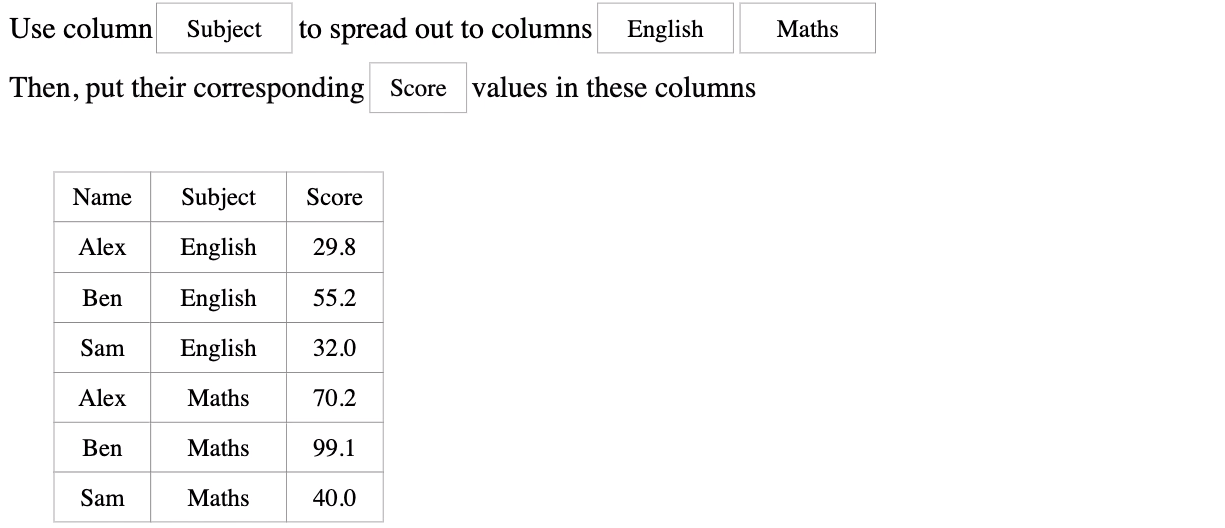
\includegraphics[scale = 0.35]{Masters-Thesis/img/spread2.png}
    \caption{Long to Wide step 2}
    \label{fig:spread2}
\end{figure}


Third, we show the structure of the resulted table. This is to give the user an idea of what the resulted table will look like. This table is currently empty and only contain column names, these empty cells will be filled in though out the animation (Fig.~\ref{fig:spread3}). 
\begin{figure}[H]
    % \centering
    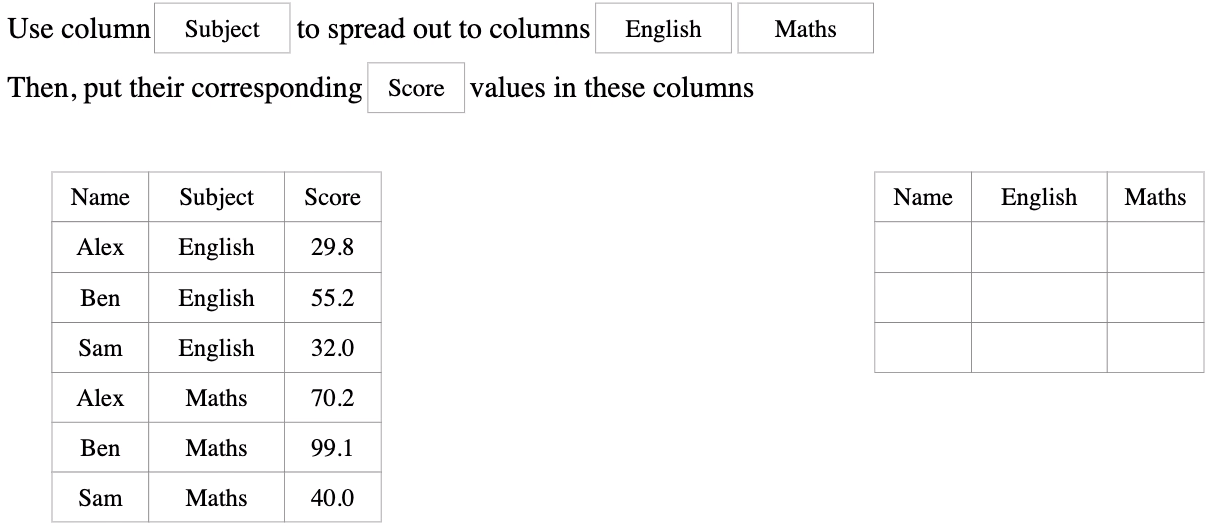
\includegraphics[scale = 0.35]{Masters-Thesis/img/spread3.png}
    \caption{Long to Wide step 3}
    \label{fig:spread3}
\end{figure}
\newpage

Fourth, we fade out the tables and the text in the background. Then we show a message informing the user that the animation will now start and that the first step is to move across unique values from the column that is neither the key or value across to the resulted table (Fig.~\ref{fig:spread4}). For example, here we show a message "Move across unique values from Name". We fade out the background to allow the user to focus on this message.
\begin{figure}[H]
    % \centering
    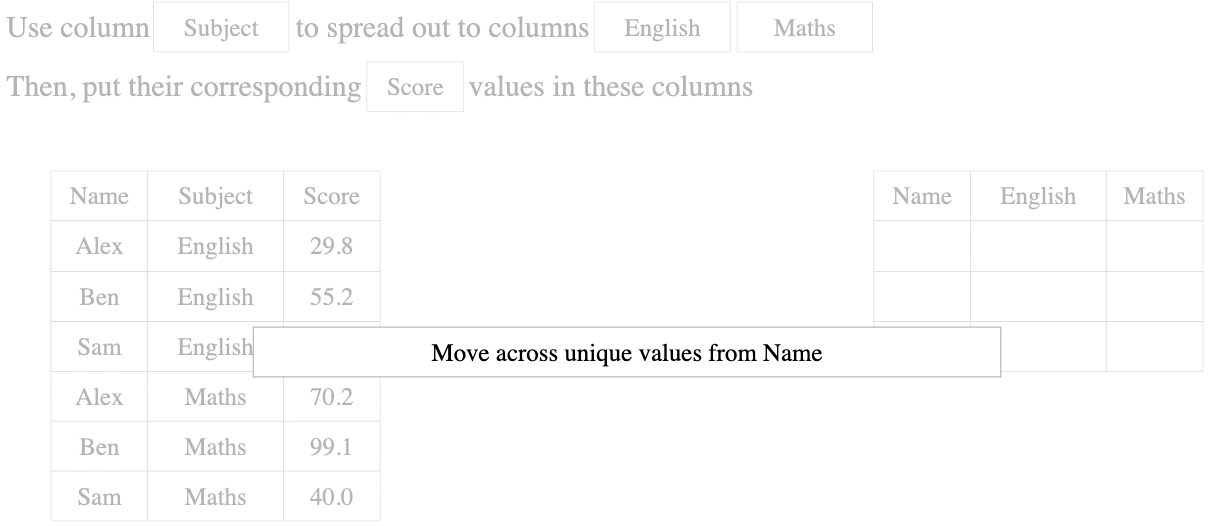
\includegraphics[scale = 0.35]{Masters-Thesis/img/spread4.png}
    \caption{Long to Wide step 4}
    \label{fig:spread4}
\end{figure}

Fifth, we flash the unique elements in the Name column, to catch the users attention Fig.~\ref{fig:spread5}).
\begin{figure}[H]
    % \centering
    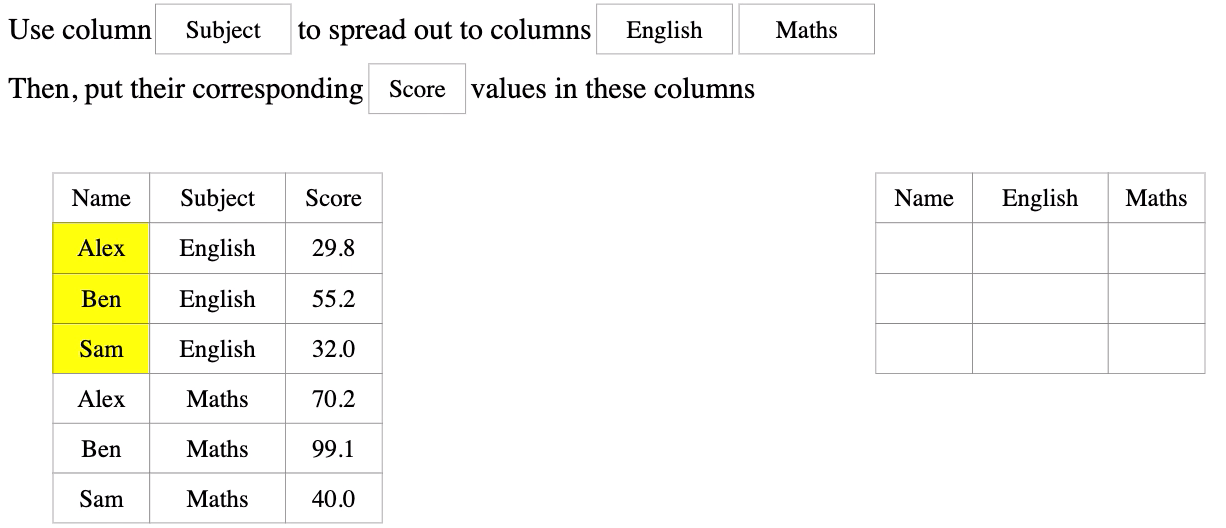
\includegraphics[scale = 0.35]{Masters-Thesis/img/spread5.png}
    \caption{Long to Wide step 5}
    \label{fig:spread5}
\end{figure}
\newpage
Sixth, we move the unique names over to the resulted table Fig.~\ref{fig:spread6}, caught mid-move).
\begin{figure}[H]
    % \centering
    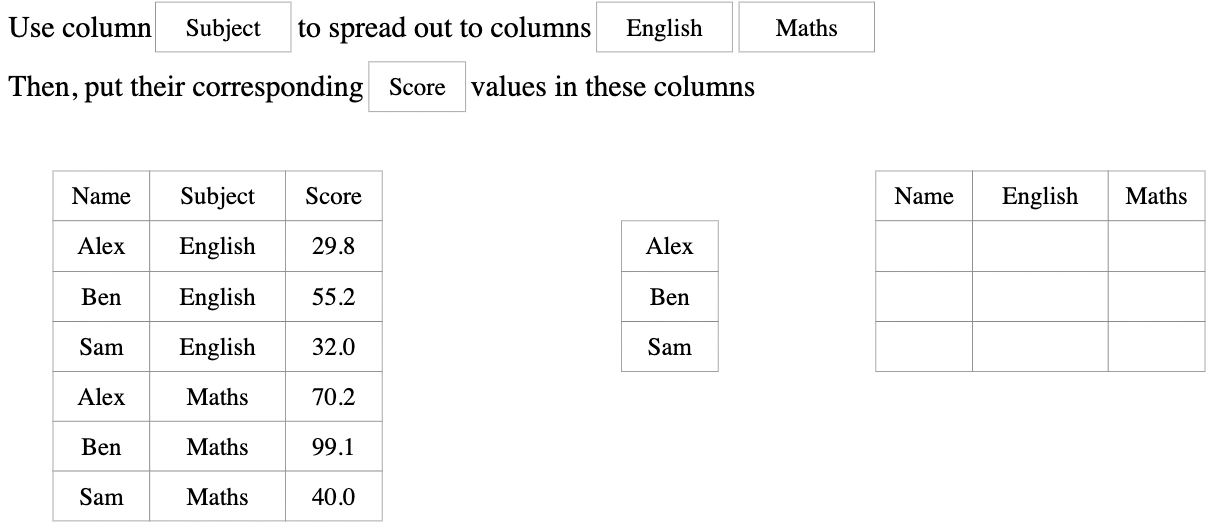
\includegraphics[scale = 0.35]{Masters-Thesis/img/spread6.png}
    \caption{Long to Wide step 6}
    \label{fig:spread6}
\end{figure}

Next, we flash the first set of unique row in the original table. Here, it is Alex and English in the original table. To catch the users attention to this row, the elements containing these values in the resulted table will also flash (Fig.~\ref{fig:spread7}). Here, we want the user to understand the relationship between the two tables. 
\begin{figure}[H]
    % \centering
    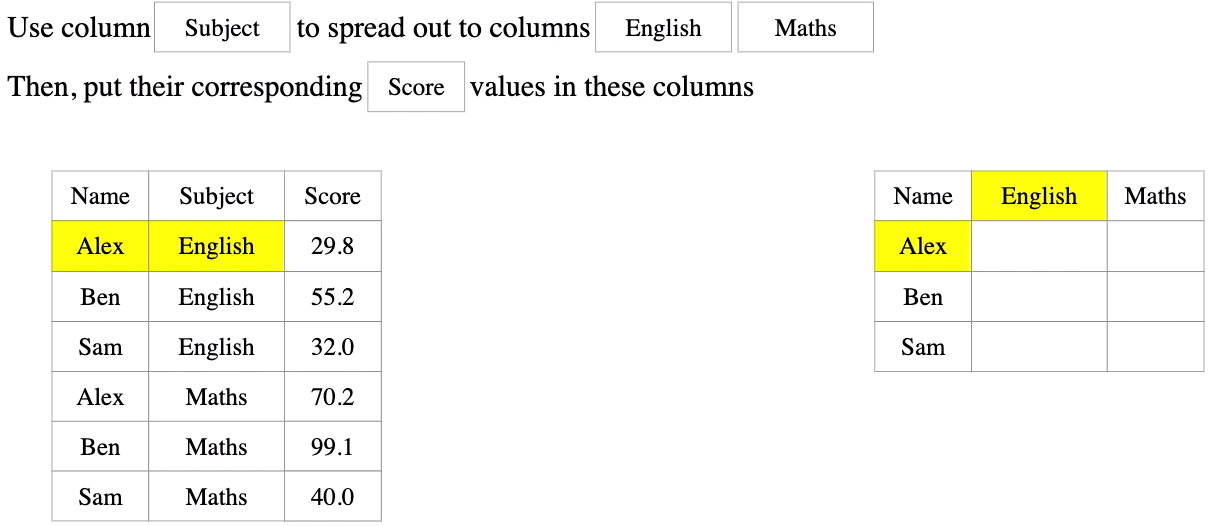
\includegraphics[scale = 0.35]{Masters-Thesis/img/spread7.png}
    \caption{Long to Wide step 7}
    \label{fig:spread7}
\end{figure}

\newpage
The values of the previously flashed rows will then move into its corresponding location in the resulted table. The correct location for this cell will be the intersect of the two flashed cells in the result table (Fig.~\ref{fig:spread8}, caught mid-move). The animation continues sequentially down the rows of the original table. 
\begin{figure}[H]
    % \centering
    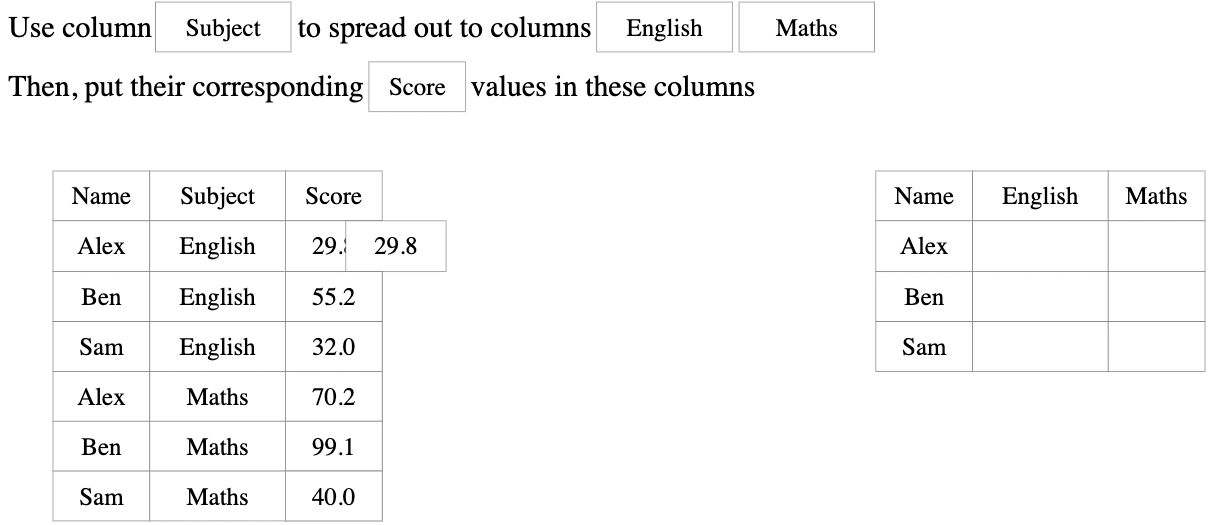
\includegraphics[scale = 0.35]{Masters-Thesis/img/spread8.png}
    \caption{Long to Wide step 8}
    \label{fig:spread8}
\end{figure}

We then do the same for Maths after we are finished with English (Fig.~\ref{fig:spread9}).
\begin{figure}[H]
    % \centering
    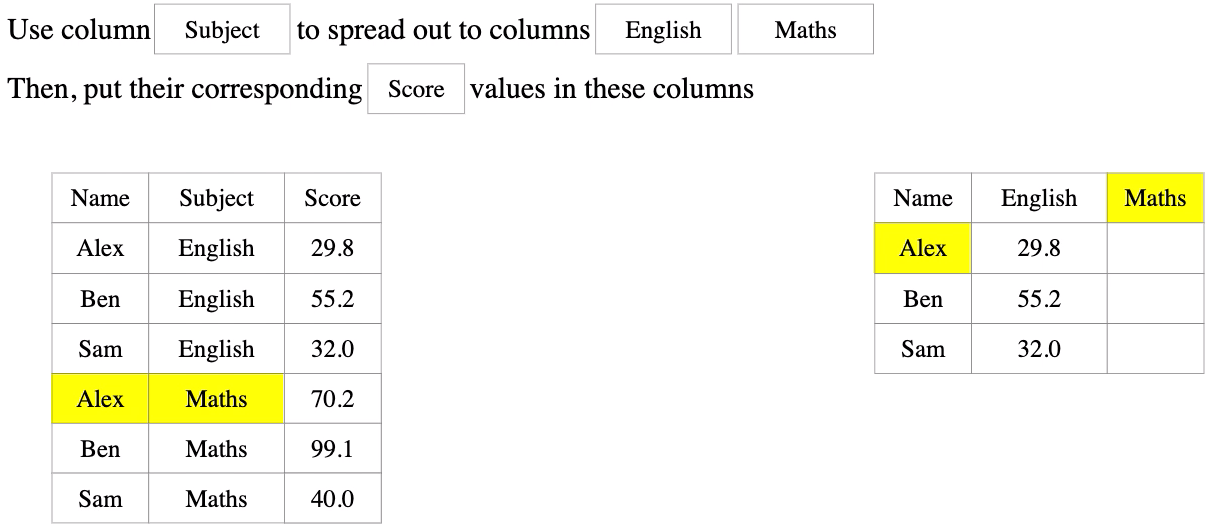
\includegraphics[scale = 0.35]{Masters-Thesis/img/spread9.png}
    \caption{Long to Wide step 9}
    \label{fig:spread9}
\end{figure}

\newpage
Lastly, when the animation finishes, the animation will stop (Fig.~\ref{fig:spread10}).
\begin{figure}[H]
    % \centering
    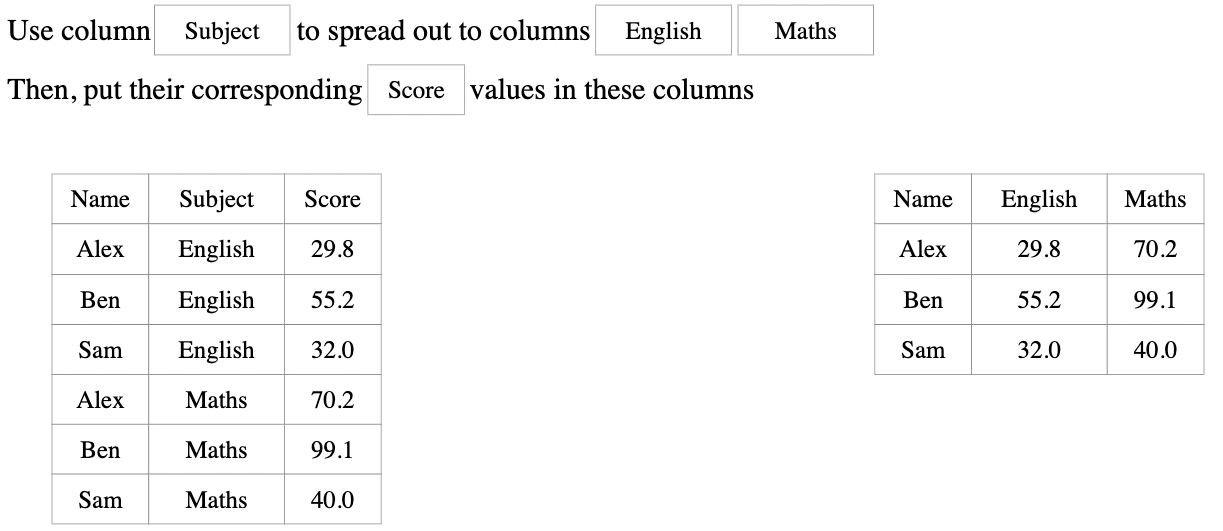
\includegraphics[scale = 0.35]{Masters-Thesis/img/spread10.png}
    \caption{Long to Wide step 10}
    \label{fig:spread10}
\end{figure}


\section{Wide to Long (Gather)}
\subsection{Logic of Wide to Long}
The logic of the wide to long transformation in the \texttt{gather} function of \textbf{tidyr} is to use the \texttt{key} and \texttt{value} column, this is the same as \texttt{gather}. However, the meaning of the \texttt{key} and \texttt{value} is different. Here, \texttt{key} is the new column name the user wishes to use to contain old column names. The \texttt{value} is the new column name to contain the old column values. An additional argument is required by \texttt{gather}, the user will also need to provide the columns they wish to transform the data on. 

\subsection{Wide to Long Animation}
Before the animation starts, we tell the user that we will create a new column to contain old column names by using a message. Here we will create a new column named Subject to contain the old column names English and Maths.

We then move elements English and Maths from the original table up to the message because we want the user to know that these are the columns we will be using during the animation (Fig.~\ref{fig:gather1}).
\begin{figure}[H]
    % \centering
    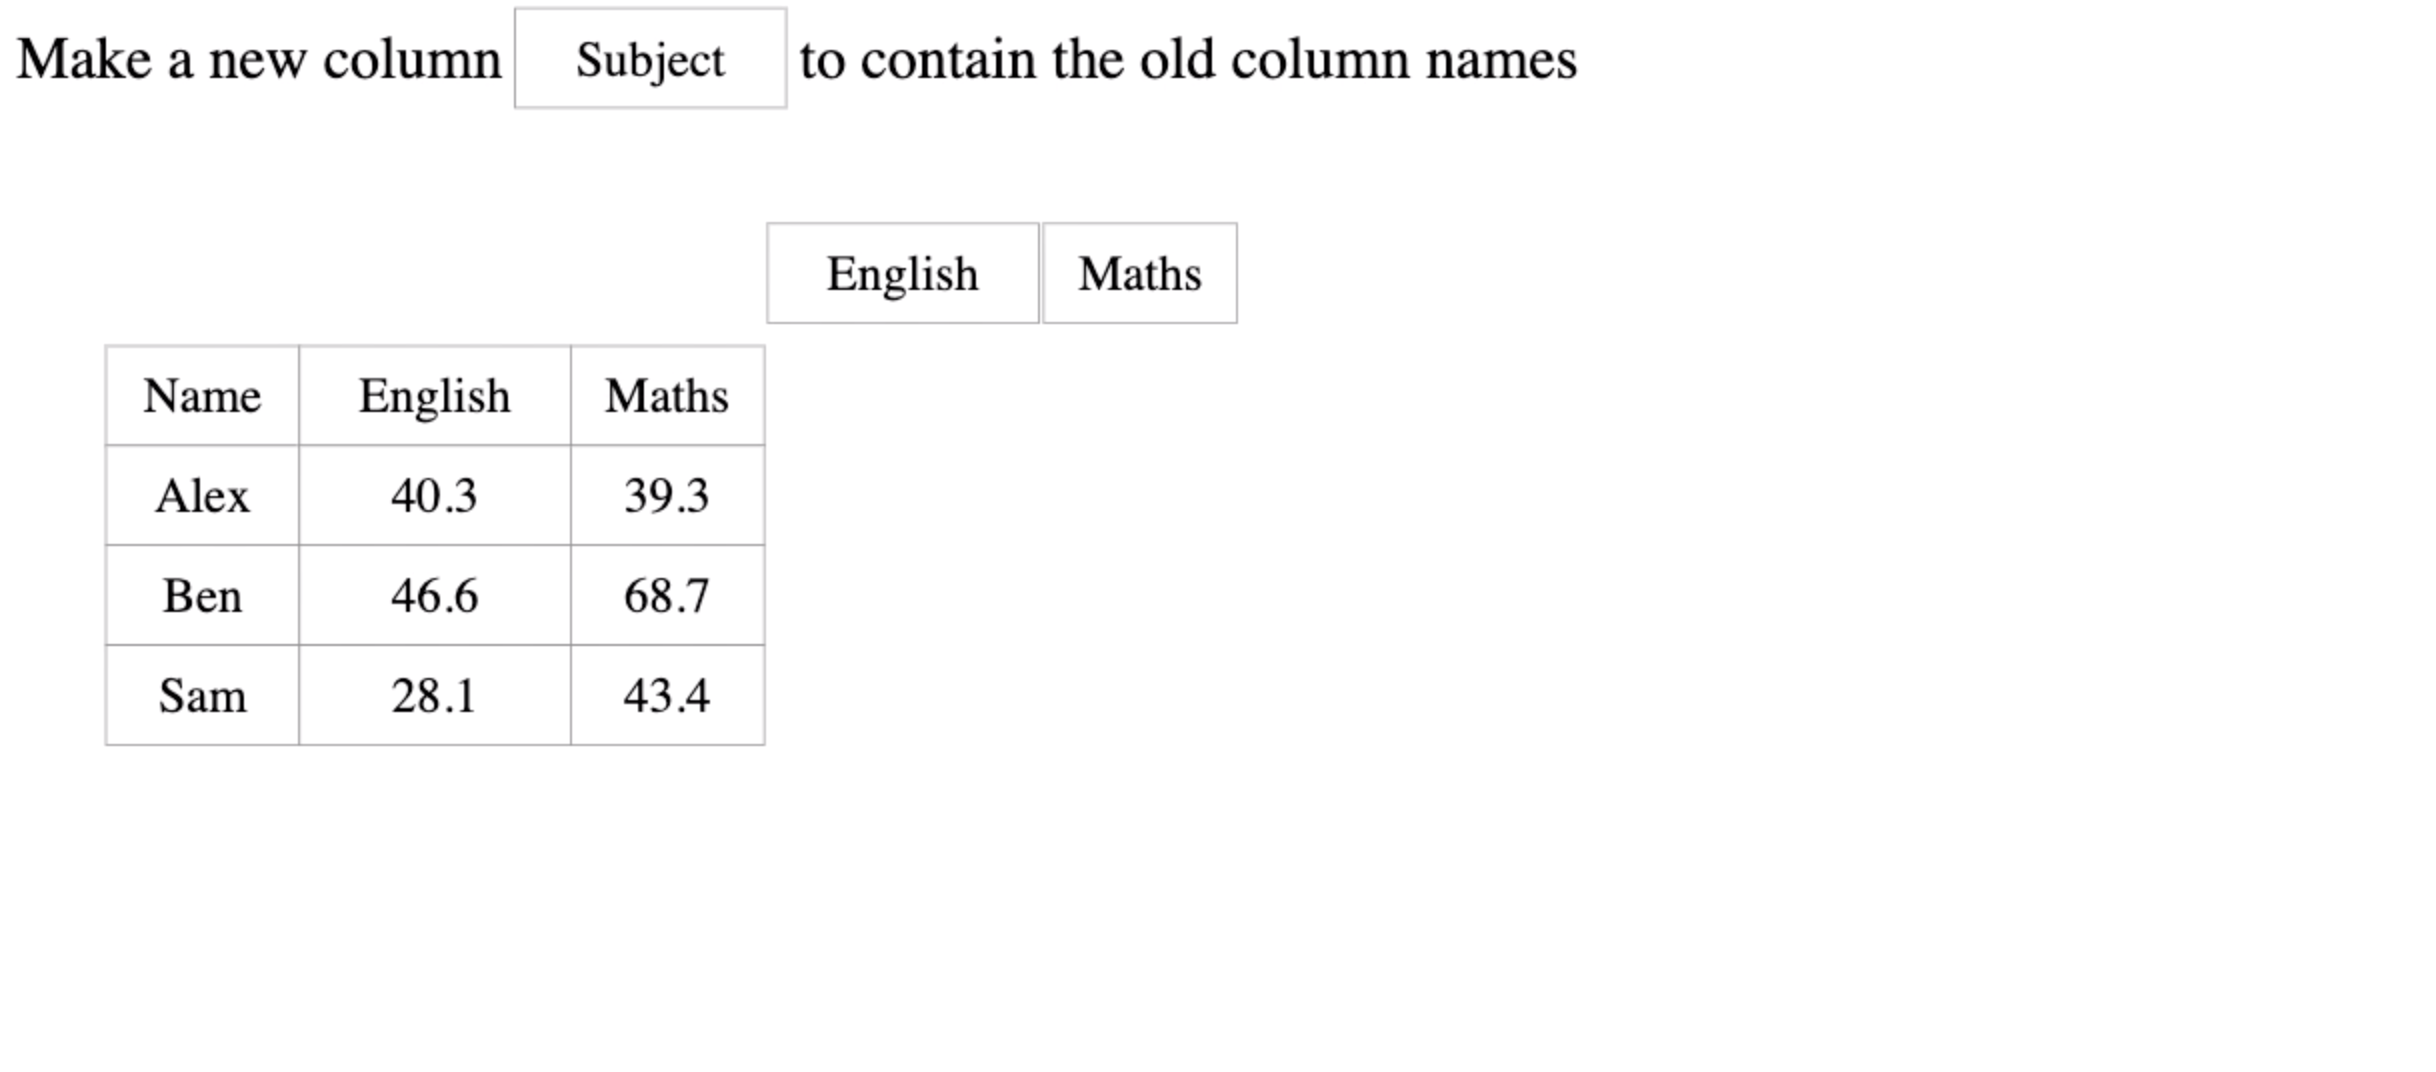
\includegraphics[scale = 0.35]{Masters-Thesis/img/gather1.png}
    \caption{Wide to Long step 1}
    \label{fig:gather1}
\end{figure}

Second, we show another message informing the user that we will create another new column to contain the old column values. Here we will create a new column in the resulted table called Score (Fig.~\ref{fig:gather2}).
\begin{figure}[H]
    % \centering
    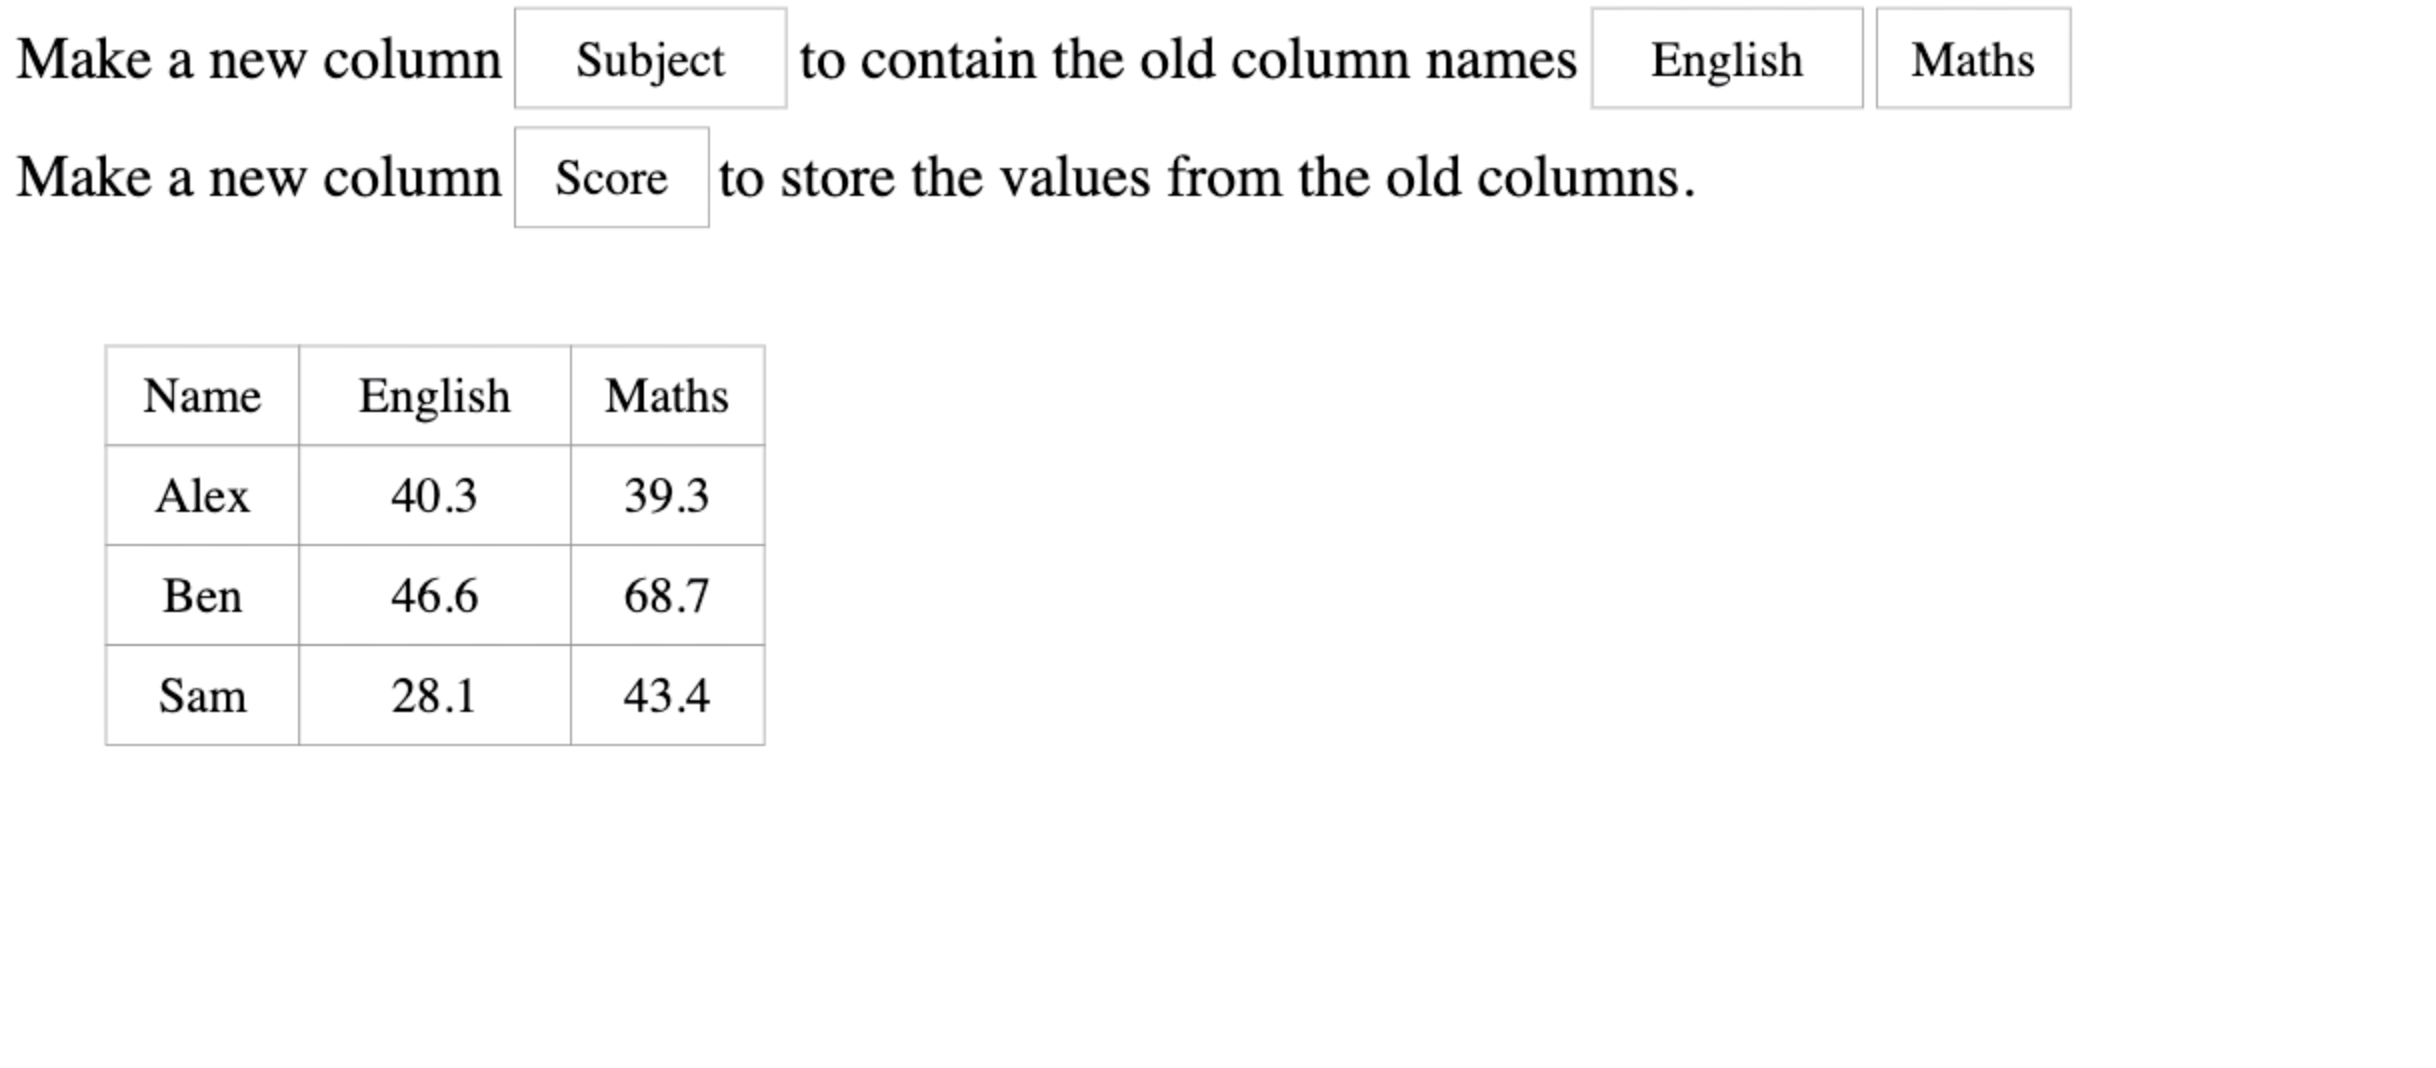
\includegraphics[scale = 0.35]{Masters-Thesis/img/gather2.png}
    \caption{Wide to Long step 2}
    \label{fig:gather2}
\end{figure}

\newpage
Third, we show the structure of the resulted table. This is to give the user an idea of what the resulted table will look like. This table is currently empty and only contain column names, these empty cells will be filled in though out the animation (Fig.~\ref{fig:gather3}).
\begin{figure}[H]
    % \centering
    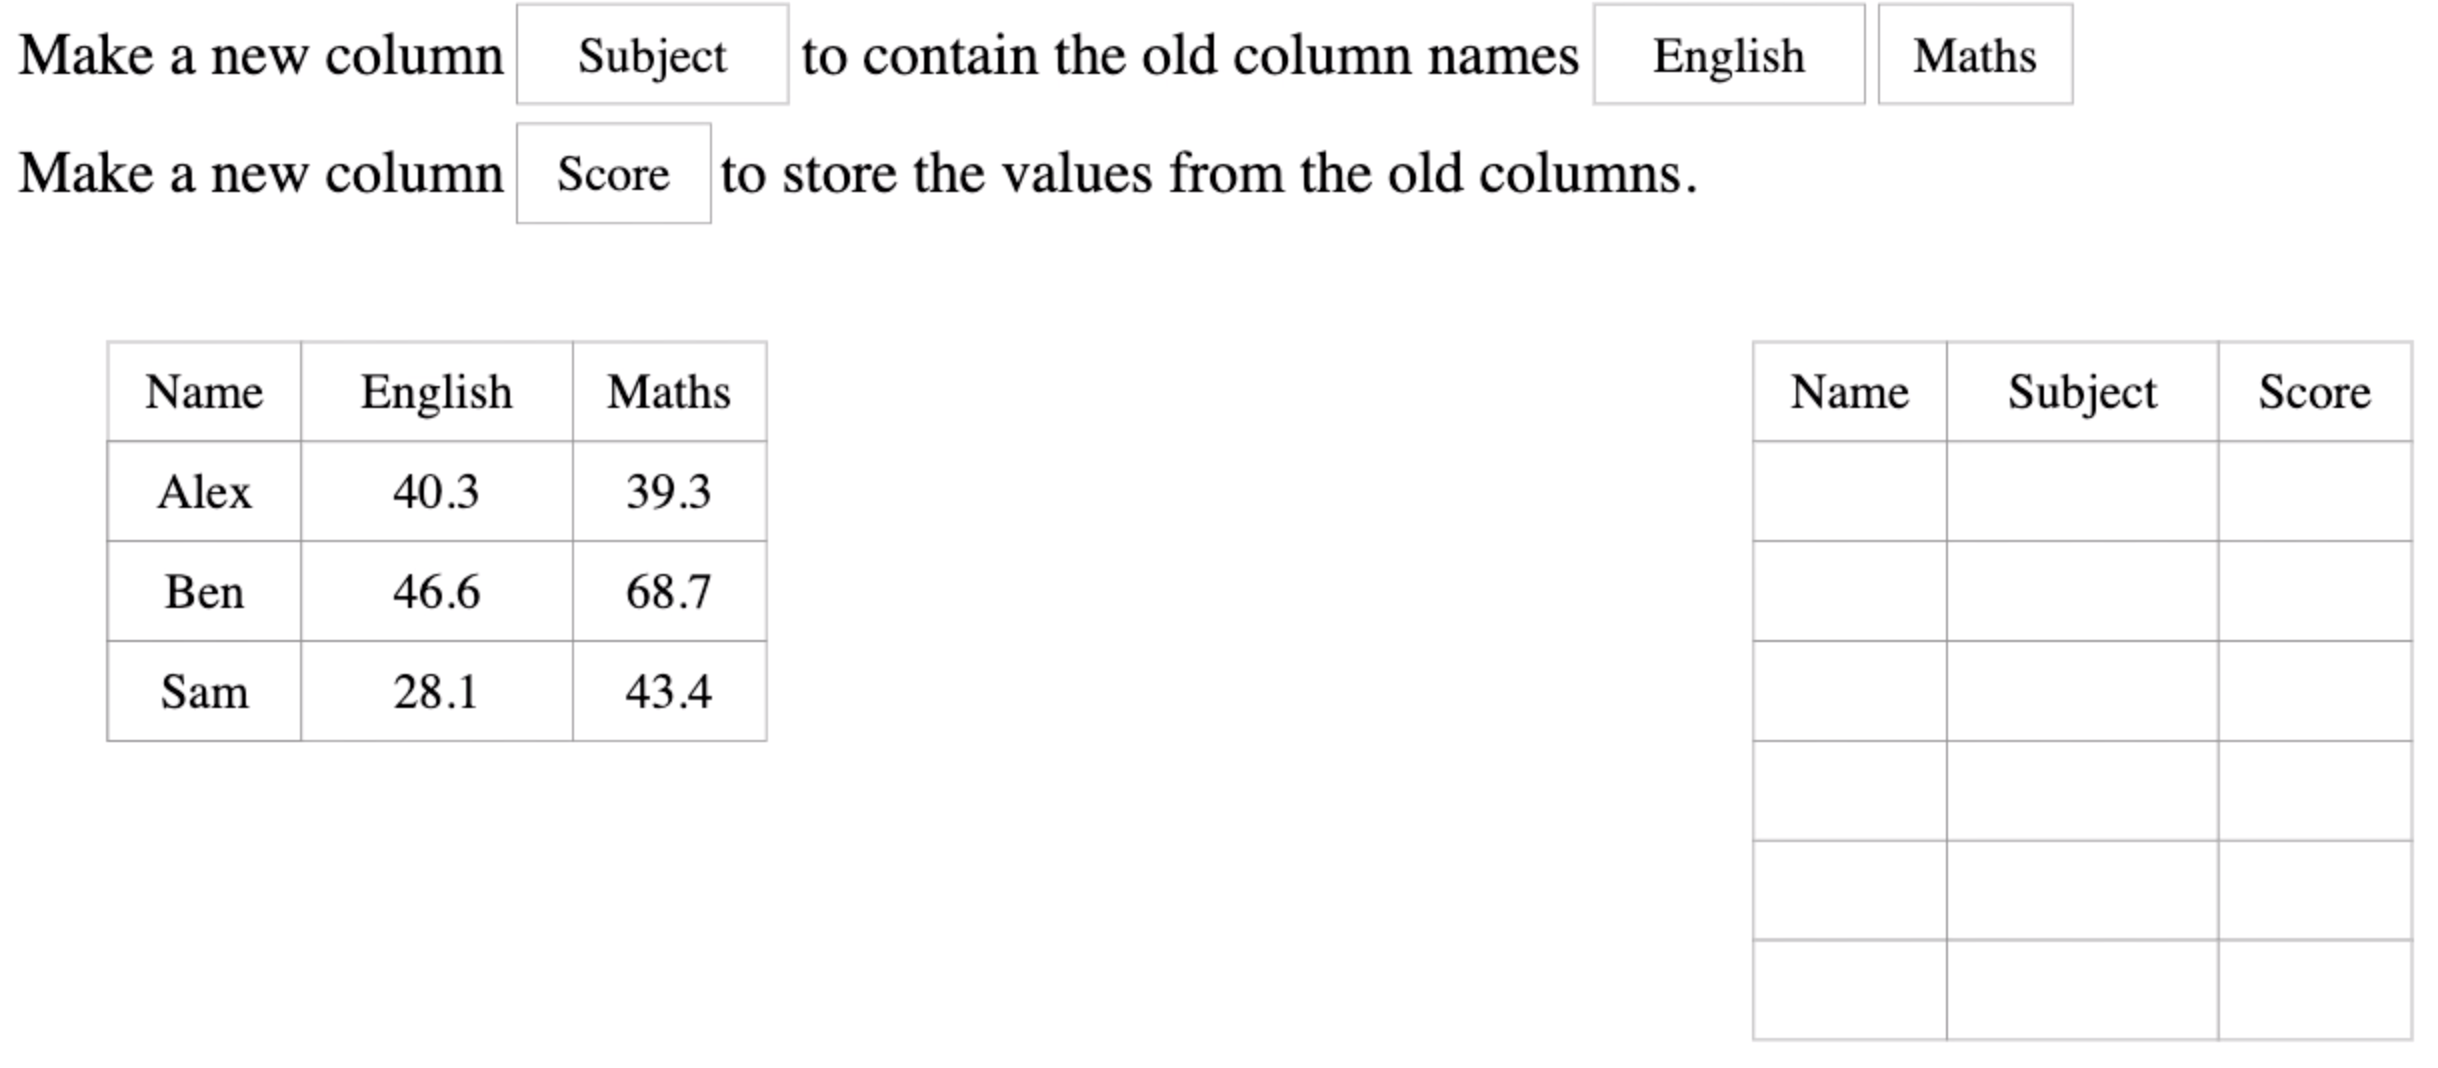
\includegraphics[scale = 0.35]{Masters-Thesis/img/gather3.png}
    \caption{Wide to Long step 3}
    \label{fig:gather3}
\end{figure}

Fourth, we fade out the tables and the text in the background and show a message informing the user that the animation will now start (Fig.~\ref{fig:gather4}). For example, here we show a message "Start wide to long transformation". We fade out the background to allow the user to focus on this message.
\begin{figure}[H]
    % \centering
    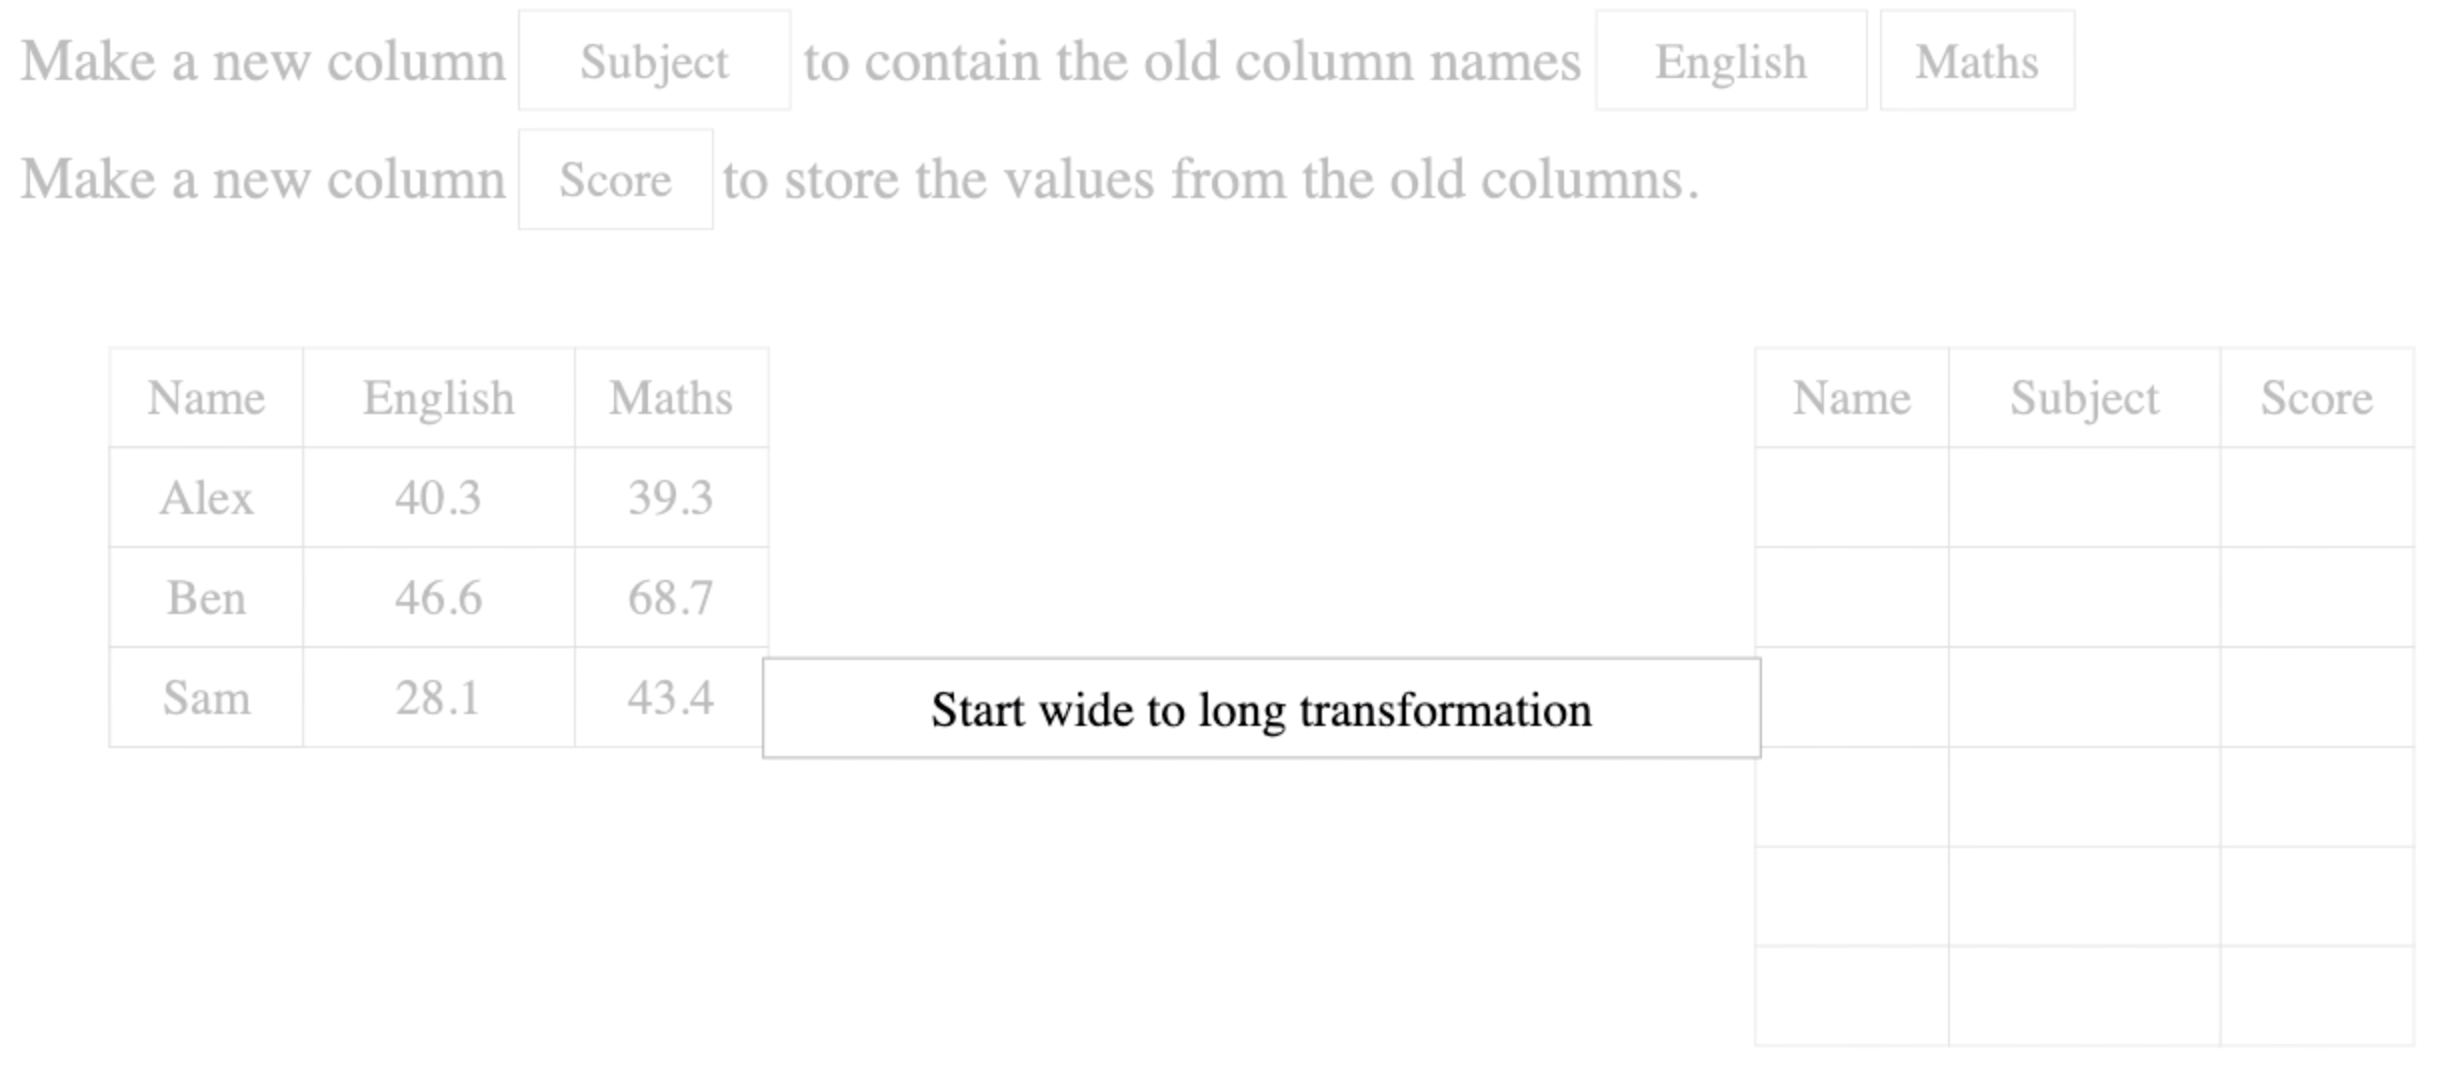
\includegraphics[scale = 0.35]{Masters-Thesis/img/gather4.png}
    \caption{Wide to Long step 4}
    \label{fig:gather4}
\end{figure}

\newpage
Fifth, we flash the column that is neither the key or the value column from both tables and link them with a line. We do this to catch the users attention.
\begin{figure}[H]
    % \centering
    \includegraphics[scale = 0.35]{Masters-Thesis/img/gather5.png}
    \caption{Wide to Long step 5}
    \label{fig:gather5}
\end{figure}

Sixth, all the values in that column will move over to the resulted table under the same column name (Fig.~\ref{fig:gather6}, caught mid-move).
\begin{figure}[H]
    % \centering
    \includegraphics[scale = 0.35]{Masters-Thesis/img/gather6.png}
    \caption{Wide to Long step 6}
    \label{fig:gather6}
\end{figure}

\newpage
Seventh, we show a message informing the user that the column name of the first column which contains the values we wish to reshape will now move over to the result table under the column they specified (key) (Fig.~\ref{fig:gather7}).
\begin{figure}[H]
    % \centering
    \includegraphics[scale = 0.35]{Masters-Thesis/img/gather7.png}
    \caption{Wide to Long step 7}
    \label{fig:gather7}
\end{figure}

Here the we flash the column name which we are currently animating. We also flash the corresponding location of where this element should go to further emphasise this process. Lastly, we animate lines to link these flashing elements to catch the users attention (Fig.~\ref{fig:gather8}). 
\begin{figure}[H]
    % \centering
    \includegraphics[scale = 0.35]{Masters-Thesis/img/gather8.png}
    \caption{Wide to Long step 8}
    \label{fig:gather8}
\end{figure}

\newpage
Next, we will move across the previously flashed column name from the original table to the locations that flashed in resulted table (Fig.~\ref{fig:gather9}). In this example, to compensate for the multiple locations that this element needs to go, we duplicate this element. The elements may or may not duplicate itself, this depends on the structure of the table.
\begin{figure}[H]
    % \centering
    \includegraphics[scale = 0.35]{Masters-Thesis/img/gather9.png}
    \caption{Wide to Long step 9}
    \label{fig:gather9}
\end{figure}

Next, we show a message to prepare the user for the next step. The next step is to move the across corresponding values that are under the previously moved column name to the resulted table. Here they are the values under in the English column (Fig.~\ref{fig:gather10}).
\begin{figure}[H]
    % \centering
    \includegraphics[scale = 0.35]{Masters-Thesis/img/gather10.png}
    \caption{Wide to Long step 10}
    \label{fig:gather10}
\end{figure}

\newpage
We then move these values across to the resulted table (Fig.~\ref{fig:gather11}, caught mid-move).
\begin{figure}[H]
    % \centering
    \includegraphics[scale = 0.35]{Masters-Thesis/img/gather11.png}
    \caption{Wide to Long step 11}
    \label{fig:gather11}
\end{figure}

After we finish animating the first column the user wishes to reshape on. We show a message informing the user that the animation will proceed with the next column (Fig.~\ref{fig:gather12}). In this example the next column is Maths, the process for this will be the same as the previously explained steps.
\begin{figure}[H]
    % \centering
    \includegraphics[scale = 0.35]{Masters-Thesis/img/gather12.png}
    \caption{Wide to Long step 12}
    \label{fig:gather12}
\end{figure}

\newpage

Lastly, when the animation finishes, the animation will stop (Fig.~\ref{fig:gather13}).

\begin{figure}[H]
    % \centering
    \includegraphics[scale = 0.35]{Masters-Thesis/img/gather13.png}
    \caption{Wide to Long step 13}
    \label{fig:gather13}
\end{figure} 
%% Chapter Template
%
\chapter{Discussion} \label{c6}

At the beginning of the report, we have discussed the limitations of a few current approaches of teaching data joining and reshaping. The traditional method of teaching with static images is limited because they are not descriptive enough. First, they usually use dummy data sets with no meaning, or data sets with vocabulary that the learners may be unfamiliar with. Second, they assume that learners can imagine data sets or the process of the transformation in their head.

Another approach found was to teach this with animations. With this approach, the user does not have to imagine the data transformation process. However, they still use data sets which are meaningless. Although, this does solve some of the limitations that the static image approach brings, we are interested to extend this.

Therefore, we attempted develop a tool which generate animations to address all the limitations mentioned above. Additionally, this tool can also be used as a resource for the data joining and reshaping module in \textbf{iNZight} to help users understand these operations in visual way.


\section{Future work}
Though some of the animations in the software already handles complicated situations while joining or reshaping data sets, we can still expand them to handle more complicated tasks. 

Additionally, we should allow students or learners to view these animations and make adjustments to the software based on their feedback.

Lastly, a \textsf{SQL} module is already under development. Although it is not ready at the moment but it is a good extension to our current joining module. 



\section{Conclusion}
We have seen multiple approaches of teaching data joining and reshaping, they turned out to be not as efficient, mostly because of the of lack explanation in the transformation process. Therefore to overcome this problem, we used technique like highlighting, line animation, fading and instructional messages. On top of that we tried to be very careful with the ordering of these operations. 

This piece of software allows users to visualise the process of data joining and reshaping. Therefore, they should be more easier to understand than most of the common approach of teaching data joining and reshaping.


\newpage
\section{Usage}
The \textbf{dataAnim} is hosted on \textsf{Github} at \href{https://github.com/chrk623/dataAnim}{https://github.com/chrk623/dataAnim}. To install \textbf{dataAnim} in \textsf{R}:

\begin{lstlisting}
 devtools::install_github("chrk623\dataAnim")
\end{lstlisting}

It is suggested to view the animations in \textbf{Chrome} and have the latest version of \textbf{Rstudio}. It is also suggested to use the most up to date version of all the dependency packages.

Lastly, the shiny interactive dashboard can be found at 

\href{https://chrk623.shinyapps.io/dataAnim_shiny/}{https://chrk623.shinyapps.io/dataAnim\_shiny/}.


 
%----------------------------------------------------------------------------------------
%	THESIS CONTENT - APPENDICES
%----------------------------------------------------------------------------------------

\appendix % Cue to tell LaTeX that the following "chapters" are Appendices

% Include the appendices of the thesis as separate files from the Appendices folder
% Uncomment the lines as you write the Appendices

% Appendix Template

\chapter{Result Tables} \label{AppendixA}

{\bf All units are in seconds.}

\section{Total}
\subsection{Numeric variable}
\begin{table}[ht]
\centering
\begin{tabular}{rrrrr}
  \hline
 & Observations & Survey & svydb.local & svydb.database \\ 
  \hline
1 & 250000 & 0.43 & 0.06 & 0.40 \\ 
  2 & 500000 & 0.88 & 0.08 & 0.41 \\ 
  3 & 750000 & 1.38 & 0.11 & 0.61 \\ 
  4 & 1000000 & 1.76 & 0.15 & 0.72 \\ 
  5 & 1250000 & 2.35 & 0.17 & 0.81 \\ 
  6 & 1500000 & 2.80 & 0.21 & 0.94 \\ 
  7 & 1750000 & 3.26 & 0.28 & 0.97 \\ 
  8 & 2000000 & 3.95 & 0.26 & 1.15 \\ 
  9 & 2500000 & - & - & 1.17 \\ 
  10 & 3000000 & - & - & 1.56 \\ 
  11 & 3500000 & - & - & 1.61 \\ 
  12 & 4000000 & - & - & 1.92 \\ 
   \hline
\end{tabular}
\end{table}

\subsection{Categorical variable with 7 levels}
\begin{table}[ht]
\centering
\begin{tabular}{rrrrr}
  \hline
 & Observations & Survey & svydb.local & svydb.database \\ 
  \hline
1 & 250000 & 0.73 & 0.22 & 1.20 \\ 
  2 & 500000 & 1.25 & 0.28 & 1.50 \\ 
  3 & 750000 & 1.87 & 0.34 & 1.76 \\ 
  4 & 1000000 & 2.58 & 0.46 & 2.03 \\ 
  5 & 1250000 & 3.10 & 0.51 & 2.28 \\ 
  6 & 1500000 & 3.94 & 0.61 & 2.65 \\ 
  7 & 1750000 & 4.42 & 0.71 & 2.92 \\ 
  8 & 2000000 & 5.27 & 0.79 & 3.20 \\ 
  9 & 2500000 & - & - & 3.63 \\ 
  10 & 3000000 & - & - & 4.25 \\ 
  11 & 3500000 & - & - & 4.67 \\ 
  12 & 4000000 & - & - & 5.21 \\ 
   \hline
\end{tabular}
\end{table}

%--------------------------------------------------------------------------------------
\section{Mean}
\subsection{Numeric variable}
\begin{table}[ht]
\centering
\begin{tabular}{rrrrr}
  \hline
 & Observations & Survey & svydb.local & svydb.database \\ 
  \hline
1 & 250000 & 0.43 & 0.09 & 0.63 \\ 
  2 & 500000 & 0.90 & 0.11 & 0.79 \\ 
  3 & 750000 & 1.35 & 0.14 & 0.96 \\ 
  4 & 1000000 & 1.86 & 0.21 & 1.24 \\ 
  5 & 1250000 & 2.13 & 0.23 & 1.31 \\ 
  6 & 1500000 & 2.77 & 0.27 & 1.48 \\ 
  7 & 1750000 & 3.26 & 0.30 & 1.62 \\ 
  8 & 2000000 & 3.60 & 0.34 & 1.85 \\ 
  9 & 2500000 & - & - & 2.09 \\ 
  10 & 3000000 & - & - & 2.39 \\ 
  11 & 3500000 & - & - & 2.66 \\ 
  12 & 4000000 & - & - & 3.09 \\ 
   \hline
\end{tabular}
\end{table}

\subsection{Categorical variable with 7 levels}
\begin{table}[ht]
\centering
\begin{tabular}{rrrrr}
  \hline
 & Observations & Survey & svydb.local & svydb.database \\ 
  \hline
1 & 250000 & 0.72 & 0.21 & 1.65 \\ 
  2 & 500000 & 1.25 & 0.35 & 2.49 \\ 
  3 & 750000 & 1.90 & 0.47 & 2.73 \\ 
  4 & 1000000 & 2.49 & 0.70 & 3.26 \\ 
  5 & 1250000 & 3.26 & 0.76 & 3.83 \\ 
  6 & 1500000 & 4.02 & 0.89 & 4.50 \\ 
  7 & 1750000 & 4.85 & 1.02 & 5.04 \\ 
  8 & 2000000 & 5.55 & 0.94 & 5.63 \\ 
  9 & 2500000 & - & - & 6.68 \\ 
  10 & 3000000 & - & - & 7.53 \\ 
  11 & 3500000 & - & - & 8.70 \\ 
  12 & 4000000 & - & - & 9.72 \\ 
   \hline
\end{tabular}
\end{table}

\newpage 

%--------------------------------------------------------------------------------------
\section{Regression}
\begin{table}[ht]
\centering
\begin{tabular}{rrrrr}
  \hline
 & Observations & Survey & svydb.local & svydb.database \\ 
  \hline
1 & 250000 & 1.18 & 0.68 & 2.95 \\ 
  2 & 500000 & 2.00 & 1.03 & 4.24 \\ 
  3 & 750000 & 3.16 & 1.30 & 5.31 \\ 
  4 & 1000000 & 4.50 & 1.31 & 6.56 \\ 
  5 & 1250000 & 5.65 & 1.65 & 7.75 \\ 
  6 & 1500000 & 6.77 & 1.97 & 8.70 \\ 
  7 & 1750000 & 8.13 & 2.24 & 10.09 \\ 
  8 & 2000000 & 9.75 & 2.68 & 10.72 \\ 
  9 & 2500000 & - & - & 12.31 \\ 
  10 & 3000000 & - & - & 14.31 \\ 
  11 & 3500000 & - & - & 16.32 \\ 
  12 & 4000000 & - & - & 18.22 \\ 
   \hline
\end{tabular}
\end{table}

%--------------------------------------------------------------------------------------
\section{Quantiles}
\begin{table}[ht]
\centering
\begin{tabular}{rrrrr}
  \hline
 & Observations & Survey & svydb.local & svydb.database \\ 
  \hline
1 & 250000 & 0.58 & 0.08 & 0.36 \\ 
  2 & 500000 & 1.16 & 0.18 & 0.51 \\ 
  3 & 750000 & 1.55 & 0.26 & 0.63 \\ 
  4 & 1000000 & 2.18 & 0.29 & 0.83 \\ 
  5 & 1250000 & 2.80 & 0.28 & 0.93 \\ 
  6 & 1500000 & 3.45 & 0.31 & 1.04 \\ 
  7 & 1750000 & 4.24 & 0.27 & 1.17 \\ 
  8 & 2000000 & 4.82 & 0.32 & 1.40 \\ 
  9 & 2500000 & - & - & 1.49 \\ 
  10 & 3000000 & - & - & 1.73 \\ 
  11 & 3500000 & - & - & 1.98 \\ 
  12 & 4000000 & - & - & 2.25 \\ 
  \hline
\end{tabular}
\end{table}

\newpage

%--------------------------------------------------------------------------------------
\section{Survey Tables}
\begin{table}[ht]
\centering
\begin{tabular}{rrrrr}
  \hline
 & Observations & Survey & svydb.local & svydb.database \\ 
  \hline
1 & 250000 & 0.18 & 0.26 & 0.67 \\ 
  2 & 500000 & 0.39 & 0.49 & 1.02 \\ 
  3 & 750000 & 0.56 & 0.69 & 1.35 \\ 
  4 & 1000000 & 0.78 & 0.76 & 1.69 \\ 
  5 & 1250000 & 0.97 & 1.00 & 2.05 \\ 
  6 & 1500000 & 1.16 & 1.11 & 2.44 \\ 
  7 & 1750000 & 1.38 & 1.37 & 2.56 \\ 
  8 & 2000000 & 1.56 & 1.47 & 2.97 \\ 
  9 & 2500000 & - & - & 3.45 \\ 
  10 & 3000000 & - & - & 4.05 \\ 
  11 & 3500000 & - & - & 4.63 \\ 
  12 & 4000000 & - & - & 5.20 \\ 
  \hline
\end{tabular}
\end{table}




%--------------------------------------------------------------------------------------
\section{Total - Replicate Weights}
\begin{table}[ht]
\centering
\begin{tabular}{rrrrr}
  \hline
 & Observations & Survey & svydb.local & svydb.database \\ 
  \hline
1 & 250000 & 3.54 & 0.46 & 2.12 \\ 
  2 & 500000 & 9.03 & 0.74 & 3.49 \\ 
  3 & 750000 & 12.31 & 1.13 & 4.81 \\ 
  4 & 1000000 & 21.57 & 1.45 & 5.86 \\ 
  5 & 1250000 & - & - & 7.10 \\ 
  6 & 1500000 & - & - & 9.34 \\ 
  7 & 1750000 & - & - & 10.62 \\ 
  8 & 2000000 & - & - & 14.75 \\ 
  \hline
\end{tabular}
\end{table}


%--------------------------------------------------------------------------------------
\section{Mean - Replicate Weights}
\begin{table}[ht]
\centering
\begin{tabular}{rrrrr}
  \hline
 & Observations & Survey & svydb.local & svydb.database \\ 
  \hline
1 & 250000 & 3.57 & 0.66 & 3.66 \\ 
  2 & 500000 & 8.69 & 0.98 & 5.68 \\ 
  3 & 750000 & 14.25 & 1.61 & 7.23 \\ 
  4 & 1000000 & 20.27 & 1.89 & 8.72 \\ 
  5 & 1250000 & - & - & 10.36 \\ 
  6 & 1500000 & - & - & 12.24 \\ 
  7 & 1750000 & - & - & 13.97 \\ 
  8 & 2000000 & - & - & 16.02 \\ 
  \hline
\end{tabular}
\end{table}

\newpage

%--------------------------------------------------------------------------------------
\section{Histogram}
\begin{table}[ht]
\centering
\begin{tabular}{rrrrr}
  \hline
 & Observations & Survey & svydb.local & svydb.database \\ 
  \hline
1 & 250000 & 0.97 & 0.58 & 1.57 \\ 
  2 & 500000 & 2.07 & 0.75 & 2.56 \\ 
  3 & 750000 & 3.14 & 0.90 & 2.84 \\ 
  4 & 1000000 & 4.03 & 1.05 & 3.49 \\ 
  5 & 1250000 & 5.15 & 1.15 & 4.12 \\ 
  6 & 1500000 & 6.12 & 1.42 & 4.79 \\ 
  7 & 1750000 & 7.50 & 1.48 & 5.24 \\ 
  8 & 2000000 & 8.57 & 1.66 & 6.05 \\ 
  9 & 2500000 & - & - & 7.03 \\ 
  10 & 3000000 & - & - & 7.94 \\ 
  11 & 3500000 & - & - & 9.15 \\ 
  12 & 4000000 & - & - & 10.34 \\ 
  \hline
\end{tabular}
\end{table}

%--------------------------------------------------------------------------------------
\section{Boxplot}
\begin{table}[ht]
\centering
\begin{tabular}{rrrrr}
  \hline
 & Observations & Survey & svydb.local & svydb.database \\ 
  \hline
1 & 250000 & 2.84 & 1.21 & 4.37 \\ 
  2 & 500000 & 4.96 & 1.39 & 5.20 \\ 
  3 & 750000 & 7.44 & 1.54 & 6.16 \\ 
  4 & 1000000 & 10.36 & 1.69 & 7.01 \\ 
  5 & 1250000 & 12.83 & 1.90 & 7.88 \\ 
  6 & 1500000 & 14.96 & 2.01 & 8.92 \\ 
  7 & 1750000 & 18.22 & 2.14 & 9.61 \\ 
  8 & 2000000 & 22.12 & 2.28 & 10.31 \\ 
  9 & 2500000 & - & - & 11.38 \\ 
  10 & 3000000 & - & - & 13.01 \\ 
  11 & 3500000 & - & - & 14.56 \\ 
  12 & 4000000 & - & - & 16.20 \\ 
  \hline
\end{tabular}
\end{table}

\newpage
%--------------------------------------------------------------------------------------
\section{Hexagon Binning}
\begin{table}[ht]
\centering
\begin{tabular}{rrrrr}
  \hline
 & Observations & Survey & svydb.local & svydb.database \\ 
  \hline
1 & 250000 & 0.41 & 0.92 & 2.05 \\ 
  2 & 500000 & 0.56 & 1.23 & 3.23 \\ 
  3 & 750000 & 0.99 & 1.53 & 4.27 \\ 
  4 & 1000000 & 1.00 & 1.97 & 5.53 \\ 
  5 & 1250000 & 1.50 & 2.17 & 6.40 \\ 
  6 & 1500000 & 1.54 & 2.47 & 7.33 \\ 
  7 & 1750000 & 1.97 & 2.61 & 8.24 \\ 
  8 & 2000000 & 2.32 & 2.92 & 9.29 \\ 
  9 & 2500000 & - & - & 10.65 \\ 
  10 & 3000000 & - & - & 12.59 \\ 
  11 & 3500000 & - & - & 14.41 \\ 
  12 & 4000000 & - & - & 16.40 \\ 
  \hline
\end{tabular}
\end{table}
%--------------------------------------------------------------------------------------

\chapter{\textsf{JavaScript} code for \textbf{dataAnim}} \label{AppendixB}

\section{Joining module}

\begin{lstlisting}
function clone_nodes() {
    d3.select(this).clone(false);
};

function get_translation(obj, type) {
    if (type == "node") {
        string = d3.select(obj).attr("transform");
    } else {
        string = obj.attr("transform");
    }
    if (string === null) {
        return ([0, 0]);
    } else {
        string = string.substring(string.indexOf("(") + 1,
            string.indexOf(")")).split(",");
        return string.map((d, i) => parseInt(d));
    }
}

function clone_everything(selector) {
    var node = d3.select(selector).node();
    return d3.select(node.parentNode.insertBefore(node
        .cloneNode(true), node.nextSibling));
};

function a_intersect(a, b) {
    var t;
    if (b.length > a.length) t = b, b = a, a = t;
    return a.filter(function (e) {
        return b.indexOf(e) > -1;
    });
}

function a_intersect2(a, b) {
    var t;
    if (b.length > a.length) t = b, b = a, a = t;
    return a.filter(function (e) {
        return b.indexOf(e) > -1;
    }).filter(function (e, i, c) {
        return c.indexOf(e) === i;
    });
}

function a_outersect(a, b) {
    return a.filter(x => !b.includes(x))
}

function arr_last(arr) {
    return arr.slice(-1)[0];
}

function arr_nth(arr, n) {
    return arr.filter(function (value, index, ar) {
        index++;
        return (index % n == 0);
    });
}

function arr_sum(arr) {
    let reducer = (accumulator, currentValue) => 
        accumulator + currentValue;
    return arr.reduce(reducer);
}

function arr_scale(arr, sc) {
    arr = arr.map((d, i) => {
        return (sc(d))
    });
    return arr;
}

function parent_setclass(sel, s_class, level) {
    for (var i = 0; i < level; i++) {
        sel = sel.select(function () {
            return this.parentNode;
        });
        sel.classed(s_class, true);
    }
}

function db_pulse_rect(nodes, col, tran_time = 1000, 
    delay_time = 0, keep_highlighted = false) {
    if (nodes.length === undefined) {
        let og_col = d3.select(nodes).style("fill");
        for (var j = 0; j < 4; j++) {
            if (j % 2 === 0) {
                d3.select(nodes)
                    .transition()
                    .duration(tran_time / 4)
                    .delay(delay_time + tran_time / 4 * j)
                    .style("fill", col);
            } else {
                d3.select(nodes)
                    .transition()
                    .duration(tran_time / 4)
                    .delay(delay_time + tran_time / 4 * j)
                    .style("fill", og_col);
            }
        }
        if (keep_highlighted === true) {
            d3.select(nodes)
                .transition()
                .delay(delay_time + tran_time)
                .style("fill", col);
        }
    } else {
        nodes.forEach(function (d, i) {
            for (var j = 0; j < 4; j++) {
                if (j % 2 === 0) {
                    d3.select(d)
                        .transition()
                        .duration(tran_time / 4)
                        .delay(delay_time + tran_time /
                            4 * j)
                        .style("fill", col);
                } else {
                    d3.select(d)
                        .transition()
                        .duration(tran_time / 4)
                        .delay(delay_time + tran_time / 
                            4 * j)
                        .style("fill", null);
                }
            }
            if (keep_highlighted === true) {
                d3.select(d)
                    .transition()
                    .delay(delay_time + tran_time)
                    .style("fill", col);
            }
        })
    }
}

function rect_mid_cord(nodes) {
    let result = new Array();
    if (nodes.length == undefined) {
        x = parseFloat(d3.select(nodes).attr("x"));
        y = parseFloat(d3.select(nodes).attr("y"));
        wd = parseFloat(d3.select(nodes).attr("width"));
        ht = parseFloat(d3.select(nodes).attr("height"));
        result.push({
            x: x + wd / 2,
            y: y + ht / 2
        });
    } else {
        nodes.forEach(function (d, i) {
            x = parseFloat(d3.select(d).attr("x"));
            y = parseFloat(d3.select(d).attr("y"));
            wd = parseFloat(d3.select(d).attr("width"));
            ht = parseFloat(d3.select(d).attr("height"));
            result.push({
                x: x + wd / 2,
                y: y + ht / 2
            });
        })
    }
    return result;
}

function nkeycol_width(id) {
    let temp_nodes = d3.select(`.${id}_rows`)
        .selectAll(`.${id}_cols:not(.${id}_cols_key`)
        .select("rect").nodes();
    let store = new Array()
    temp_nodes.forEach(function (d, i) {
        store.push(parseFloat(d3.select(d).attr("width")));
    })
    return store;
}

function link_rect_line(base, base_key_rect_xy, dest = -1, 
    qm_align = "left", tran_time = 2000, delay_time = 0,
    msg, removeall = true, msg_pause = 2000) {
    let rect_height = parseFloat(d3.select("rect")
        .attr("height"));
    let rect_width = null;
    d3.select(".x_rows")
        .selectAll("rect")
        .each(function (d, i) {
            cur_width = d3.select(this).attr("width");
            if (i == 0) {
                rect_width = cur_width;
            } else {
                if (cur_width < rect_width) {
                    rect_width = cur_width;
                }
            }
        });
    let cond = dest;
    let qm_tran_time = tran_time * 0.8;
    let qm_delay_time = qm_tran_time;
    let base_node = base;
    let dest_node = dest;
    let mid_cord = tbl_mid_cord("x", "y");
    let msg_trantime = tran_time / 2;
    db_pulse_rect(base_node, "yellow", tran_time, delay_time
        , true);
    if (cond != -1) {
        db_pulse_rect(dest_node, "yellow", tran_time, 
            delay_time, true);
    }
    base = rect_mid_cord(base)[0];
    if (cond == -1) {
        dest = [tbl_mid_cord("x", "y")]
    } else {
        dest = rect_mid_cord(dest);
    }
    if (qm_align == "right") {
        qm_class = "qm";
    } else if (qm_align === "left") {
        qm_class = "qm2";
    }
    let link_line = new Array();
    dest.forEach(function (d, i) {
        link_line_i = d3.select("svg")
            .append("line")
            .attr("x1", base_key_rect_xy["x"])
            .attr("y1", base_key_rect_xy["y"])
            .attr("x2", base_key_rect_xy["x"])
            .attr("y2", base_key_rect_xy["y"]);
        link_line.push(link_line_i);
    })
    if (cond != -1) {
        link_line.forEach(function (d, i) {
            d.transition()
                .delay(delay_time)
                .duration(tran_time)
                .attr("x2", dest[i]["x"])
                .attr("y2", dest[i]["y"]);
        })
        delay_time = delay_time + tran_time;
    } else {
        link_line.forEach(function (d, i) {
            d.transition()
                .delay(delay_time)
                .duration(tran_time)
                .attr("x2", dest[i]["x"])
                .attr("y2", dest[i]["y"]);
        })
        delay_time = delay_time + tran_time;
        qm = d3.select("svg")
            .append("text")
            .attr("class", qm_class)
            .attr("x", dest[0]["x"])
            .attr("y", dest[0]["y"])
            .style("font-size", 0);
        qm.transition()
            .delay(delay_time)
            .duration(qm_tran_time)
            .text("?")
            .style("font-size", rect_height * 1.5)
        delay_time = delay_time + qm_tran_time;
    }
    if (msg["msg"] != undefined) {
        let msg_x = new Array();
        let msg_y = new Array();
        link_line.forEach(function (d, i) {
            msg_x.push((dest[0]["x"] + base_key_rect_xy["x"])
                / 2);
            msg_y.push((dest[0]["y"] + base_key_rect_xy["y"]) 
                / 2);
        });
        msg_x = arr_sum(msg_x) / msg_x.length;
        msg_y = arr_sum(msg_y) / msg_y.length;
        delay_time = msg_box(msg_x, msg_y, rect_width * 3
            ,rect_height * 2, msg["msg"], delay_time, 
            msg_trantime, msg_pause);
        delay_time = delay_time + tran_time / 2;
    }
    link_line.forEach(function (d, i) {
        d.transition()
            .delay(delay_time)
            .on("end", function () {
                d3.select(this)
                    .remove();
                d3.selectAll("rect")
                    .style("fill", null);
            });
    })
    if (cond == -1) {
        qm.transition()
            .delay(delay_time)
            .on("end", function () {
                d3.select(this)
                    .remove();
            });
    }
    return delay_time;
}

function link_rect_line2(base, base_key_rect_xy, dest = -1
    ,qm_align = "left", tran_time = 2000, delay_time = 0,
    msg, removeall = true) {
    if (msg["msg"] != undefined) {
        msg_trantime = tran_time * 0.15;
        msg_pausetime = tran_time * 0.35;
        tran_time = tran_time / 2;
    }
    if (dest == -1) {
        qm_tran_time = tran_time * 0.2;
        tran_time = tran_time * 0.8;
    }
    let rect_height = parseFloat(d3.select("rect")
        .attr("height"));
    let rect_width = null;
    d3.select(".x_rows")
        .selectAll("rect")
        .each(function (d, i) {
            cur_width = d3.select(this).attr("width");
            if (i == 0) {
                rect_width = cur_width;
            } else {
                if (cur_width < rect_width) {
                    rect_width = cur_width;
                }
            }
        });
    let cond = dest;
    let base_node = base;
    let dest_node = dest;
    let mid_cord = tbl_mid_cord("x", "y");
    db_pulse_rect(base_node, "yellow", tran_time, delay_time
        ,true);
    if (cond != -1) {
        db_pulse_rect(dest_node, "yellow", tran_time,
            delay_time, true);
    }
    base = rect_mid_cord(base)[0];
    if (cond == -1) {
        dest = [tbl_mid_cord("x", "y")]
    } else {
        dest = rect_mid_cord(dest);
    }
    if (qm_align == "right") {
        qm_class = "qm";
    } else if (qm_align === "left") {
        qm_class = "qm2";
    }
    let link_line = new Array();
    dest.forEach(function (d, i) {
        link_line_i = d3.select("svg")
            .append("line")
            .attr("x1", base_key_rect_xy["x"])
            .attr("y1", base_key_rect_xy["y"])
            .attr("x2", base_key_rect_xy["x"])
            .attr("y2", base_key_rect_xy["y"]);
        link_line.push(link_line_i);
    })
    if (cond != -1) {
        link_line.forEach(function (d, i) {
            d.transition()
                .delay(delay_time)
                .duration(tran_time)
                .attr("x2", dest[i]["x"])
                .attr("y2", dest[i]["y"]);
        })
        delay_time = delay_time + tran_time;
    } else {
        link_line.forEach(function (d, i) {
            d.transition()
                .delay(delay_time)
                .duration(tran_time)
                .attr("x2", dest[i]["x"])
                .attr("y2", dest[i]["y"]);
        })
        delay_time = delay_time + tran_time;
        qm = d3.select("svg")
            .append("text")
            .attr("class", qm_class)
            .attr("x", dest[0]["x"])
            .attr("y", dest[0]["y"])
            .style("font-size", 0);
        qm.transition()
            .delay(delay_time)
            .duration(qm_tran_time)
            .text("?")
            .style("font-size", rect_height * 1.5)
        delay_time = delay_time + qm_tran_time;
    }
    if (msg["msg"] != undefined) {
        let msg_x = new Array();
        let msg_y = new Array();
        link_line.forEach(function (d, i) {
            msg_x.push((dest[0]["x"] + base_key_rect_xy["x"])
                / 2);
            msg_y.push((dest[0]["y"] + base_key_rect_xy["y"]) 
                / 2);
        });
        msg_x = arr_sum(msg_x) / msg_x.length;
        msg_y = arr_sum(msg_y) / msg_y.length;
        delay_time = msg_box(msg_x, msg_y, rect_width * 3
            ,rect_height * 2, msg["msg"], delay_time, 
            msg_trantime, msg_pausetime);
    }
    link_line.forEach(function (d, i) {
        d.transition()
            .delay(delay_time)
            .on("end", function () {
                d3.select(this)
                    .remove();
                d3.selectAll("rect")
                    .style("fill", null);
            });
    })
    if (cond == -1) {
        qm.transition()
            .delay(delay_time)
            .on("end", function () {
                d3.select(this)
                    .remove();
            });
    }
    return delay_time;
}

function link_rectline_only(base, base_key_rect_xy
    ,dest = -1, tran_time = 2000, delay_time = 0) {
    let rect_height = parseFloat(d3.select("rect")
        .attr("height"));
    let cond = dest;
    let qm_tran_time = tran_time * 0.8;
    let return_delay = delay_time + tran_time;
    let base_node = base;
    let dest_node = dest;
    base = rect_mid_cord(base)[0];
    if (cond == -1) {
        dest = [tbl_mid_cord("x", "y")]
        return_delay = return_delay + qm_tran_time;
    } else {
        dest = rect_mid_cord(dest)
    }
    dest.forEach(function (d, i) {
        link_line = d3.select("svg")
            .append("line");
        link_line.attr("x1", base_key_rect_xy["x"])
            .attr("y1", base_key_rect_xy["y"])
            .attr("x2", base_key_rect_xy["x"])
            .attr("y2", base_key_rect_xy["y"]);
        link_line
            .transition()
            .duration(tran_time)
            .delay(delay_time)
            .attr("x2", d["x"])
            .attr("y2", d["y"])
            .on("end", function () {
                link_line = d3.select(this);
                d3.select("svg")
                    .transition()
                    .delay(1000)
                    .on("end", function () 
                        {
                        link_line.remove()
                    })
            });
    })
    return return_delay;
}

function move_rect(to_sel, from_node, tran_time
    ,delay_time) {
    parent_setclass(d3.select(from_node), "moved", 1);
    d3.select(from_node)
        .select("rect")
        .classed("moved", true)
        .transition()
        .delay(delay_time)
        .duration(tran_time)
        .on("start", function (d, i) {
            d3.select(this)
                .clone(true);
        })
        .attr("x", to_sel.attr("x"))
        .attr("y", to_sel.attr("y"))
        .attr("width", to_sel.attr("width"))
        .on("end", function (d, i) {
            d3.select(this)
                .remove();
        });
}

function move_text(to_sel, from_node, tran_time, delay_time) {
    d3.select(from_node)
        .select("text")
        .classed("moved", true)
        .transition()
        .delay(delay_time)
        .duration(tran_time)
        .on("start", function (d, i) {
            d3.select(this)
                .clone(true);
        })
        .attr("x", to_sel.attr("x"))
        .attr("y", to_sel.attr("y"))
        .on("end", function (d, i) {
            d3.select(this)
                .remove();
        });
}

function movexy_rect(node, x, y, width
    ,tran_time, delay_time,
    insert_txt = null, remove = false) {
    if (y === null) {
        y = d3.select(node)
            .select("rect")
            .attr("y")
    }
    if (insert_txt != null || insert_txt != undefined) {}
    node = d3.select(node)
        .select("rect")
        .clone(true)
        .node();
    d3.select(".x_rows")
        .insert(function () {
            return node;
        })
    d3.select(node).classed("moved", true)
        .transition()
        .delay(delay_time)
        .duration(tran_time)
        .attr("x", x)
        .attr("y", y)
        .attr("width", width)
        .on("end", function (d, i) {
            if (remove === true) {
                d3.select(this)
                    .remove();
            }
        });
}

function movexy_text(node, x, y, adj_y = null, width, 
        tran_time, delay_time,insert_txt = null, 
            remove = false) {
    parent_setclass(d3.select(node), "moved", 1);
    if (y === null) {
        y = d3.select(node)
            .select("text")
            .attr("y");
    }
    if (adj_y !== null) {
        y = y + 0.5 * adj_y;
    }
    node = d3.select(node)
        .select("text")
        .clone(true);
    node.classed("moved", true)
        .transition()
        .delay(delay_time)
        .duration(tran_time)
        .attr("x", parseInt(x) + 0.5 * width)
        .attr("y", y)
        .on("end", function (d, i) {
            if (remove === true) {
                d3.select(this)
                    .remove();
            }
        });
}

function movexy_cell(node, rx, ry, tx, ty, adj_ty = null, 
    width ,tran_time, delay_time, location = null, 
    msg = undefined, remove = false) {
    rnode = d3.select(node)
        .select("rect")
        .clone(true)
        .node();
    tnode = d3.select(node)
        .select("text")
        .clone(true)
        .node();
    if (ry === null) {
        ry = d3.select(node)
            .select("rect")
            .attr("y")
    }
    d3.select(rnode)
        .transition()
        .delay(delay_time)
        .duration(tran_time)
        .attr("x", rx)
        .attr("y", ry)
        .attr("width", width)
        .on("end", function (d, i) {
            if (location != null) {
                base = this;
                d3.select(location)
                    .insert(function () {
                        return base;
                    })
            }
        });
    if (ty === null) {
        ty = d3.select(node)
            .select("text")
            .attr("y");
    }
    if (adj_ty !== null) {
        ty = ty + 0.5 * adj_ty;
    }
    d3.select(tnode)
        .transition()
        .delay(delay_time)
        .duration(tran_time)
        .attr("x", parseFloat(tx) + 0.5 * width)
        .attr("y", ty)
        .on("end", function (d, i) {
            if (location != null) {
                base = this;
                d3.select(location)
                    .insert(function () {
                        return base;
                    })
            }
        });
    return delay_time + tran_time;
}

function movexy_cell_wobj(node, xy, height, width
    ,tran_time, delay_time,
    location = null, join_type = "left", msg = undefined
        ,remove = false) {
    let xy_keys = Object.keys(xy);
    let return_delay = 0;
    if (node.length == undefined) {
        node = [node];
    }
    if (node[0] == undefined) {
        if (join_type === "left" || join_type === "complete") {
            xy[0]["x"].forEach(function (d, i) {
                na_rects(d, xy[0]["y"], width[i], height, 
                `.x_rows:nth-child(${location[0]})`,
                tran_time, delay_time)
            });
        } else if (join_type === "inner") {
            d3.select(`.x_rows:nth-child(${location[0]})`)
                .classed("remove_row", true)
                .transition()
                .delay(delay_time)
                .duration(tran_time)
                .style("opacity", 0);
        }
        return_delay = return_delay + tran_time;
        return return_delay;
    }
    node.forEach(function (d, i) {
        cur_node = d3.select(node[i]).selectAll(".y_cols:not
            (.y_cols_key)").nodes();
        cur_node.forEach(function (d2, j) {
            movexy_cell(d3.select(d2).node(), xy[i]["x"][j]
                ,xy[i]["y"], xy[i]["x"][j],
                xy[i]["y"], height, width[j], tran_time
                    ,delay_time,
                `.x_rows:nth-child(${location[i]})`, msg
                    ,false)
        });
    })
    return_delay = return_delay + tran_time;
    return return_delay;
}

function tbl_mid_cord(c1, c2, xy = true) {
    right = d3.select(`.${c2}_tbl>.${c2}_rows:last-child`)
        .select("rect");
    right_x = parseInt(right.attr("x"));
    right_y = parseInt(right.attr("y")) + 
        parseInt(right.attr("height"));
    left = d3.select(`.${c1}_tbl`)
        .select(`.${c1}_cols_last`)
        .select("rect");
    left_y = parseInt(left.attr("y"));
    if (xy === true) {
        let right_rect = d3.select(".y_rows")
            .selectAll(".y_cols:not(.y_cols_key)")
            .nodes();
        let right_w = 0;
        right_rect.forEach(function (d, i) {

            cur_rect = d3.select(d).select("rect");
            right_w = right_w + parseFloat(cur_rect
                .attr("width"));
        })
        left_x = parseInt(left.attr("x")) + parseInt(left
            .attr("width")) + right_w;
    } else {
        left_x = parseInt(left.attr("x")) + parseInt(left
            .attr("width"));
    }

    return ({
        x: (right_x + left_x) / 2,
        y: (right_y + left_y) / 2
    });
}

function get_newcol_xy(initial_prep, totbl_topright
    ,fromtbl_nkey_wd, height) {
    totbl_topright[1] = totbl_topright[1] + height;
    let new_x = [totbl_topright[0]];
    fromtbl_nkey_wd.map((d, i) => {
        if (i > 0) {
            new_x.push(new_x[i - 1] + fromtbl_nkey_wd[i - 1]);
        }
    });
    let s_cnt = -1;
    let store_obj = new Object();
    Object.keys(initial_prep).forEach(function (d, i, k) {
        cur_data = initial_prep[d];
        if (i === 0) {
            cur_store = [{
                x: new_x,
                y: totbl_topright[1]
            }]
        } else {
            cur_store = new Array();
            for (var j = 0; j < cur_data.length; j++) {
                if (j > 0) {
                    s_cnt++;
                }
                cur_store.push({
                    x: new_x,
                    y: totbl_topright[1] +
                        height * (cur_data[j]["row"] + 
                            s_cnt)
                })
            }
        }
        store_obj[i + 1] = cur_store;
    });
    return store_obj;
}

function get_newcol_xyw_cn(to_tbl_id, from_tbl_id) {
    let new_width = new Array()
    let new_xy = tbl_tr_cord(to_tbl_id);
    let new_x = [new_xy[0]];
    let new_y = parseFloat(d3.select(`.${to_tbl_id}_tbl`)
        .select("rect").attr("y"));
    let nodes2move = d3.select(`.${from_tbl_id}_rows`)
        .selectAll(`.${from_tbl_id}_cols
            :not(.${from_tbl_id}_cols_key)`)
        .nodes();
    nodes2move.forEach(function (d, i) {
        cur_rect = d3.select(d).select("rect");
        new_width.push(parseFloat(cur_rect.attr("width")));
        if (i > 0) {
            new_x.push(new_x[i - 1] +
                parseFloat(d3.select(nodes2move[i - 1])
                    .select("rect")
                    .attr("width")))
        }
    })
    return {
        x: new_x,
        y: new_y,
        width: new_width
    };
}

function tbl_tr_cord(c) {
    tr_rect = d3.select(`.${c}_tbl`)
        .select(`.${c}_cols_last > rect`);
    x = parseFloat(tr_rect.attr("x"));
    y = parseFloat(tr_rect.attr("y"));
    wd = parseFloat(tr_rect.attr("width"));
    return [x + wd, y];
}

function tbl_bl_cord(c) {
    last_row = d3.select(".x_tbl")
        .select(".x_rows:last-of-type");
    first_rect = last_row.select("rect");
    return {
        x: parseFloat(first_rect.attr("x")),
        y: parseFloat(first_rect.attr("y")) +
        parseFloat(first_rect.attr("height"))
    }
}

function msg_box(x, y, width = null, height = null, msg
    ,start_time = 0, tran_time = 1000
        ,pause_time = 1000, center = true) {
    if (width == null) {
        d3.select(".x_rows")
            .selectAll("rect")
            .each(function (d, i) {
                cur_width = d3.select(this).attr("width");
                if (i == 0) {
                    width = cur_width;
                } else {
                    if (cur_width < width) {
                        width = cur_width;
                    }
                }
            });
        width = width * 3;
    }
    if (height == null) {
        height = parseFloat(d3.select("rect")
            .attr("height")) * 2;
    }
    if (center === true) {
        x = x - width / 2;
        y = y - height / 2;
    }
    let txt_x = x + width / 2;
    let txt_y = y + height / 2;
    let txt_fontsize = d3.select("text")
        .style("font-size");
    msgbox = d3.select("svg")
        .append("g")
        .attr("class", "msgbox");
    if (msg == "gettimeonly") {
        msgbox
            .style("opacity", 0)
    }
    msgbox.append("rect")
        .transition()
        .delay(start_time)
        .duration(tran_time)
        .attr("x", x)
        .attr("y", y)
        .attr("width", width)
        .attr("height", height);
    msgbox.append("text")
        .attr("x", txt_x)
        .attr("y", txt_y)
        .style("font-size", 0)
        .transition()
        .delay(start_time)
        .duration(tran_time)
        .style("font-size", txt_fontsize)
        .text(msg);
    delay_time = start_time + tran_time;
    msgbox
        .transition()
        .delay(delay_time)
        .duration(pause_time)
        .on("end", function () {
            d3.select(this)
                .remove();
        })
    return delay_time + pause_time;
}

function na_rects(x, y, width, height, location = null
    ,tran_time = 1000, delay_time = 0) {
    let svg = d3.select("svg");
    svg
        .append("rect")
        .attr("class", "na_rects")
        .attr("x", x)
        .attr("y", y)
        .attr("width", 0)
        .attr("height", 0)
        .transition()
        .duration(tran_time)
        .delay(delay_time)
        .attr("width", width)
        .attr("height", height)
        .on("end", function () {
            base = this;
            d3.select(location)
                .insert(function () {
                    return base;
                })
        });
    svg
        .append("text")
        .attr("class", "na_rects")
        .attr("x", x + 0.5 * width)
        .attr("y", y + 0.5 * height)
        .text("NA")
        .style("font-size", 0)
        .transition()
        .delay(delay_time)
        .duration(tran_time)
        .style("font-size", height * 0.55)
        .on("end", function () {
            base = this;
            d3.select(location)
                .insert(function () {
                    return base;
                })
        });;
}

function keycol_anim(to_tbl, from_tbl, speed = 1
    ,start_time = 0) {
    let keypath_tran_time = 1500 / speed;
    let key_opacity_tran_time = 1000 / speed;
    let rectpulse_tran_time = 1500 / speed;
    let join_tran_time = 2000 / speed;
    let delay_time = start_time;
    let key_name = d3.select(`.${to_tbl}_cols_key`)
        .select("text").text();
    let to_keycol_node = d3.select(`.${to_tbl}_cols_key`)
        .node();
    let from_keycol_node = d3.select(`.${from_tbl}_cols_key`)
        .node();
    let to_keycol_node2 = d3.select(`.${to_tbl}_cols_key`)
        .nodes();
    let from_keycol_node2 = d3.select(`.${from_tbl}_cols_key`)
        .nodes();
    let to_keyrect_sel = d3.select(to_keycol_node)
        .select("rect");
    let from_keyrect_sel = d3.select(from_keycol_node)
        .select("rect");
    let to_keytext_sel = d3.select(to_keycol_node)
        .select("text");
    let to_nkeycol_nodes = d3.select(`.${to_tbl}_rows`)
        .selectAll(`.${to_tbl}_cols
            :not(.${to_tbl}_cols_key)`)
        .nodes();
    let from_nkeycol_nodes = d3.select(`.${from_tbl}_rows`)
        .selectAll(`.${from_tbl}_cols
            :not(.${from_tbl}_cols_key)`)
        .nodes();
    let to_nkeycol_nodes2 =
        d3.selectAll(`.${to_tbl}_cols
            :not(.${to_tbl}_cols_key)`)
        .nodes();
    let from_nkeycol_nodes2 =
        d3.selectAll(`.${from_tbl}_cols
            :not(.${from_tbl}_cols_key)`)
        .nodes();
    let height = parseFloat(to_keyrect_sel.attr("height"));
    let keylink_nodes = new Array();
    to_keyrect_sel.nodes().forEach(function (d, i) {
        one = [
            parseFloat(to_keyrect_sel.attr("x")) +
            parseFloat(to_keyrect_sel.attr("width")) / 2,
            parseFloat(to_keyrect_sel.attr("y"))
        ];
        two = [one[0], height * 0.6];
        three = [
            parseFloat(from_keyrect_sel.attr("x")) +
            parseFloat(from_keyrect_sel.attr("width")) / 2,
            two[1]
        ];
        four = [three[0], one[1]];
        draw_path = `M ${one} ${two} ${three} ${four}`;
        path_sel = d3.select("svg")
            .append("path")
            .attr("class", "key_col_link")
            .attr("d", draw_path)
            .attr("fill", "none")
            .attr('fill-opacity', 0);
        keylink_nodes.push(path_sel.node())
    })
    d3.selectAll(to_nkeycol_nodes2)
        .transition()
        .delay(delay_time)
        .duration(key_opacity_tran_time)
        .style("opacity", 0.5);
    d3.selectAll(from_nkeycol_nodes2)
        .transition()
        .delay(delay_time)
        .duration(key_opacity_tran_time)
        .style("opacity", 0.5);
    delay_time = delay_time + key_opacity_tran_time;
    keylink_nodes.forEach(function (d, i) {
        length = d.getTotalLength();
        d3.select(d)
            .attr("stroke-dasharray", length + " " + length)
            .attr("stroke-dashoffset", length)
            .transition()
            .delay(delay_time)
            .duration(keypath_tran_time)
            .attr("stroke-dashoffset", 0)
    });
    d3.select("svg")
        .append("text")
        .attr("id", "joinby_text")
        .attr("x", (one[0] + four[0]) / 2)
        .attr("y", one[1])
        .style("opacity", 0)
        .style("font-size", d3.select("text")
            .style("font-size"))
        .style("alignment-baseline", "hanging")
        .text(`Joining by ${key_name}`)
        .transition()
        .duration(keypath_tran_time)
        .delay(delay_time)
        .style("opacity", 1)
        .on("end", function () {
            d3.select(this)
                .remove();
        })
    delay_time = delay_time + keypath_tran_time;
    db_pulse_rect(from_keyrect_sel.nodes(), "yellow"
        ,rectpulse_tran_time, delay_time)
    db_pulse_rect(to_keyrect_sel.nodes(), "yellow"
        ,rectpulse_tran_time, delay_time)
    delay_time = delay_time + rectpulse_tran_time;
    let new_xyd = get_newcol_xyw_cn("x", "y")
    from_nkeycol_nodes.forEach(function (d, i) {
        movexy_cell(d, new_xyd["x"][i], new_xyd["y"]
        ,new_xyd["x"][i],
            new_xyd["y"], height, new_xyd["width"][i]
                ,join_tran_time, delay_time,
            ".x_rows", false)
    })
    delay_time = delay_time + join_tran_time;
    d3.selectAll(to_nkeycol_nodes2)
        .transition()
        .delay(delay_time)
        .duration(key_opacity_tran_time)
        .style("opacity", 1);
    d3.selectAll(from_nkeycol_nodes2)
        .transition()
        .delay(delay_time)
        .duration(key_opacity_tran_time)
        .style("opacity", 1);
    delay_time = delay_time + key_opacity_tran_time;
    return d3.select("svg")
        .transition()
        .delay(delay_time);
}

function shift_row_down(tbl_id, tbl_sel, row2shift
    ,shiftdown_times, height,
    tran_time, delay_time) {
    tbl_sel.selectAll(`.${tbl_id}_rows:nth-child
        (n+${row2shift + 1}`)
        .each(function (d, i) {
            cur_rect_y = d3.select(this)
                .selectAll("rect")
                .attr("y");
            cur_text_y = d3.select(this)
                .selectAll("text")
                .attr("y");
            d3.select(this)
                .selectAll("rect")
                .transition()
                .duration(tran_time)
                .delay(delay_time)
            d3.select(this)
                .selectAll("text")
                .transition()
                .duration(tran_time)
                .delay(delay_time)
                .attr("y", parseFloat(cur_text_y) + 
                    shiftdown_times * height);
        });
    tbl_sel.select(`.${tbl_id}_rows:nth-child(${row2shift}`)
        .transition()
        .delay(delay_time)
        .on("end", function () {
            for (var j = shiftdown_times; j >= 1; j--) {
                cur_row = d3.select(this).clone(true);
                cur_row.style("opacity", 0);
                cur_row.transition()
                    .duration(tran_time / 2)
                    .style("opacity", 1);
                cur_rect_y = parseFloat(cur_row.select("rect")
                    .attr("y"));
                cur_text_y = parseFloat(cur_row.select("text")
                    .attr("y"));
                cur_col = cur_row.selectAll(`.${tbl_id}_cols`);
                cur_col.selectAll("rect")
                    .transition()
                    .duration(tran_time * 0.7)
                    .attr("y", cur_rect_y + height * j);
                cur_col.selectAll("text")
                    .transition()
                    .duration(tran_time * 0.7)
                    .attr("y", cur_text_y + height * j);
            }
        })
    return delay_time + tran_time;
}

function iso_tbl(join_type = "left", height, speed = 1
    ,start_time = 0) {
    let tran_time = 1500 / speed;
    let delay_time = start_time;
    let to_tbl = "x";
    let from_tbl = "y";
    if (join_type === "right") {
        let to_tbl = "y";
        let from_tbl = "x";
    }
    let svg_wh = {
        height: parseFloat(d3
            .select("svg").attr("height")),
        width: parseFloat(d3
            .select("svg").attr("width"))
    }
    let to_tbl_tl = {
        x: parseFloat(d3.select
            (`.${to_tbl}_cols > rect`)
                .attr("x")),
        y: parseFloat(d3.select
            (`.${to_tbl}_cols > rect`)
                .attr("y"))
    }
    let to_tbl_width = 0;
    d3.select(`.${to_tbl}_rows`).selectAll("rect").nodes()
        .forEach(function (d, i) {
            to_tbl_width += parseFloat(d3.select(d)
                .attr("width"));
        });
    let to_tbl_height = height *
    parseInt(d3.selectAll(".x_rows").nodes().length);
    d3.selectAll(`.${to_tbl}_rows:not(.remove_row)`)
        .nodes().length;
    let translate_xy = {
        x: svg_wh["width"] / 2 - to_tbl_width / 
            2 - to_tbl_tl["x"],
        y: svg_wh["height"] / 2 - to_tbl_height / 
            2 - to_tbl_tl["y"]
    };
    d3.selectAll(`.${from_tbl}_tbl, path, .remove_row`)
        .transition()
        .delay(delay_time)
        .duration(tran_time)
        .style("opacity", 0)
        .on("end", function () {
            d3.select(this)
                .remove();
        });
    delay_time = delay_time + tran_time;
    d3.select(`.${to_tbl}_tbl`)
        .transition()
        .delay(delay_time)
        .duration(tran_time)
        .attr("transform", `translate(${translate_xy["x"]},
        ${translate_xy["y"]})`);
    d3.selectAll(`.${to_tbl}_rows:not(.remove_row)`).nodes()
        .forEach(function (d, i) {
            d3.select(d)
                .selectAll("rect")
                .transition()
                .delay(delay_time)
                .duration(tran_time)
                .attr("y", to_tbl_tl["y"] + height * i);
            d3.select(d)
                .selectAll("text")
                .transition()
                .delay(delay_time)
                .duration(tran_time)
                .attr("y", to_tbl_tl["y"] + height * i 
                    + height / 2);
        })
    d3.select(`.${to_tbl}_rows`)
        .selectAll("text")
        .transition()
        .delay(delay_time)
        .duration(tran_time)
        .style("font-weight", "bold");

    delay_time = delay_time + tran_time;

    return d3.select("svg")
        .transition().delay(delay_time);
}

function draw_table(input, x_start, y_start, x_cord, width
    ,height, name, key_col) {
    let y_cord = 0 - height;
    let tbl_name = `${name}_tbl`;
    let row_name = `${name}_rows`
    let col_name = `${name}_cols`
    let key_name = d3.keys(input);
    let new_x_cord = x_cord.map((d, i) => d + x_start);
    let new_y_cord = Array();
    d3.select("svg")
        .append("g")
        .attr("class", tbl_name)
        .selectAll("g")
        .data(input)
        .enter()
        .append("g")
        .attr("class", row_name)
        .each(function (d, i) {
            var header = d3.select(this);
            new_y_cord.push(height * i + y_start);
            d3.keys(d).forEach(function (key, j) {
                header
                    .append("rect")
                    .attr("width", width[j])
                    .attr("height", height)
                    .attr("x", new_x_cord[j])
                    .attr("y", new_y_cord[i])
                    .style("fill", "white");
            });
        });
    d3.selectAll(`.${row_name}`)
        .selectAll("rect").each(function (d, i) {
            var el = this;
            d3.select(el.parentNode)
                .insert("g")
                .attr("class", col_name)
                .append(function () {
                    return el;
                });
        });
    var key_rect = d3.selectAll(`.${col_name}:nth-of-type
        (${key_col})`).nodes();
    d3.selectAll(key_rect)
        .classed(`${col_name}_key`, true)
        .classed("key_col", true);
    var last_rect = d3.selectAll
        (`.${col_name}:last-of-type`).nodes();
    d3.selectAll(last_rect)
        .classed(`${col_name}_last`, true)
        .classed("last_col", true);
    d3.selectAll(`.${row_name}`)
        .each(function (d, i) {
        input_i = input[i];
        input_i_key = d3.keys(input_i);
        d3.select(this).selectAll(`.${col_name}`)
            .each(function (d, j) {
            d3.select(this)
                .append("text")
                .text(input_i[input_i_key[j]])
                .attr("x", new_x_cord[j] + width[j] * 0.5)
                .attr("y", new_y_cord[i] + height * 0.5)
                .style("font-size", height * 0.5);
        })
    });
    d3.select(`.${row_name}`).selectAll("text")
        .style("font-size", height * 0.5);
    return ({
        x: new_x_cord,
        y: new_y_cord
    });
};

function join_anim(data, speed = 1, join_type = "left"
    ,gray_out = true) {
    if (join_type == "left" || join_type == "complete") {
        return_delay = join_anim_left(data, speed, 
            join_type = "left", gray_out);
    } else if (join_type = "inner") {
        return_delay = join_anim_inner(data, speed, 
            join_type = "inner", gray_out);
    }
    return d3.select("svg")
        .transition().delay(return_delay);
}

function join_anim_left(data, speed = 1, join_type = "inner"
    ,gray_out = true) {
    let og_xtbl = d3.select(".x_tbl");
    let left_kcol_node = d3.select(".x_tbl")
        .selectAll(".x_cols_key").nodes();
    let right_kcol_node = d3.select(".y_tbl")
        .selectAll(".y_cols_key").nodes();
    let left_row_nodes = d3.selectAll(".x_rows").nodes();
    let right_row_nodes = d3.selectAll(".y_rows").nodes();
    let xy_tbl_cord = tbl_mid_cord("x", "y");
    let height = parseFloat(d3.select("rect").attr("height"));
    let xtbl_topright = tbl_tr_cord("x");
    let ytbl_nkey_wd = nkeycol_width("y");
    let new_xy = get_newcol_xy(data, xtbl_topright
        ,ytbl_nkey_wd, height);
    let shift_cnt = 1;
    let shift_adjy = 0;
    let line_tran_time = 1200 / speed;
    let line_tran_time2 = 2400 / speed;
    let shiftdown_time = 1500 / speed;
    let join_tran_time = 1500 / speed;
    let na_action_time = 1000 / speed;
    let gray_time = 200 / speed;
    let delay_time = 0;

    let r_link_rect = {};
    d3.keys(data).forEach(function (d, i) {
        let cur_r_link_rect = new Array();
        if (data[d].length > 1) {
            data[d].forEach(function (d2, i2) {
                cur_r_link_rect.push(d3.select
                    (right_kcol_node[d2["dest"]])
                    .select("rect").node());
                r_link_rect[i] = cur_r_link_rect;
            })
        } else {
            if (data[d][0]["dest"] == -1) {
                cur_r_link_rect = -1;
            } else {
                cur_r_link_rect = d3.select
                    (right_kcol_node[data[d][0]["dest"]])
                    .select("rect").node();
            }
        }
        r_link_rect[i] = cur_r_link_rect;
    })
    d3.keys(data).forEach(function (d, i) {
        d3.select("svg")
            .transition()
            .delay(delay_time)
            .on("end", function () {
                msg = {
                    msg: data[d][0].msg
                }
                ind = data[d][0]["row"];
                cur_left_rect = d3.select
                    (left_kcol_node[ind])
                    .select("rect").node();
                cur_left_rect_xy = rect_mid_cord
                    (cur_left_rect)[0];
                cur_left_rect_xy["y"] = cur_left_rect_xy["y"];
                if (msg["msg"] != undefined) {
                    cur_linetime = line_tran_time2;
                } else {
                    cur_linetime = line_tran_time;
                }
                return_delay = link_rect_line2(cur_left_rect
                    ,cur_left_rect_xy, r_link_rect[i], "right",
                    cur_linetime, 0, msg, removeall = true)
                data[d].forEach(function (d2, i2) {
                    cur_rows2move = d3.select
                        (right_row_nodes[d2["dest"]])
                        .selectAll(".y_cols:not(.y_cols_key)")
                            .nodes();
                    cur_rows2move.forEach(function (d33, i3) {
                        cur_rectwidth = d3.select(d33)
                            .select("rect").attr("width");
                        movexy_cell(cur_rows2move[i3]
                            ,new_xy[1][0]["x"][i3]
                                ,new_xy[1][0]["y"]
                                + shift_adjy * height
                                    ,new_xy[1][0]["x"][i3],
                            new_xy[1][0]["y"] + shift_adjy 
                                * height, height, 
                                    cur_rectwidth, 
                                    join_tran_time, 
                                    return_delay,
                    `.x_rows:nth-child(${data[d][i2]["row"]
                                + shift_cnt})`, {
                                msg: undefined
                            }, false);
                    })
                    shift_adjy = shift_adjy + 1

                })
                if (data[d].length > 1) {
                    shift_row_down("x", og_xtbl
                        ,data[d][0]["row"] + shift_cnt
                            ,data[d].length - 1, height, 
                                shiftdown_time
                                ,return_delay);
                    shift_cnt = shift_cnt + data[d].length - 1;
                }
            })
        if (data[d][0].msg != undefined) {
            delay_time = delay_time + line_tran_time2 
                + join_tran_time + 200 / speed;
        } else {
            delay_time = delay_time + line_tran_time 
                + join_tran_time + 200 / speed;
        }
        if (data[d][0]["dest"] == -1) {
            d3.select("svg")
                .transition()
                .delay(delay_time)
                .on("end", function () {
                    new_xy[d][0]["x"].forEach(function 
                        (d2, i2) {
                        na_rects(d2, new_xy[d][0]["y"]
                            , ytbl_nkey_wd[i2], height,
                            `.x_rows:nth-child(${
                                data[d][0]["row"] 
                                + shift_cnt})`, 
                                na_action_time, 0);
                    })
                })
            delay_time = delay_time + na_action_time;
        } else {
            data[d].forEach(function (d2, i2) {
                if (d2["dest"] != -1) {
                    d3.select(right_row_nodes[d2["dest"]])
                        .transition()
                        .delay(delay_time)
                        .duration(gray_time)
                        .style("opacity", 0.3);
                }
            })
            delay_time = delay_time + gray_time;
        }
    })
    return delay_time;
}

function comjoin_final(data, speed = 1, start_time = 0) {
    let row2move = data.row2move;
    let col_ind = data.col_ind;
    if (row2move.length < 0) {
        return 0;
    }
    let tran_time = 1500 / speed;
    let lineqm_time = tran_time / 2;
    let na_time = (tran_time / 1.5) / speed;
    let delay_time = start_time;
    let num_xrows = d3.selectAll(".x_rows").nodes().length;
    let xtbl_bl = tbl_bl_cord("x");
    let xtbl_tr = tbl_tr_cord("x");
    let height = parseFloat(d3.select("rect").attr("height"));
    let last_xrow_rects = d3.select(".x_rows:last-of-type")
        .selectAll("rect")
        .nodes();
    let og_xcols = d3.select(".x_rows")
        .selectAll(".x_cols")
        .nodes();
    let newcols_ind = og_xcols.length + 1;
    let xcol_key_ind = d3.select(".x_rows")
    let new_x = new Array();
    let new_width = new Array();
    let msg_tran_time = 1500 / speed;
    let msg_pause_time = 1500 / speed;
    col_ind.forEach(function (d, i) {
        new_x.push(parseFloat
            (d3.select(last_xrow_rects[d - 1]).attr("x")));
        new_width.push(parseFloat
            (d3.select(last_xrow_rects[d - 1]).attr("width")));
    })
    let new_y = new Array();
    row2move.forEach(function (d, i) {
        if (i === 0) {
            new_y.push(xtbl_bl["y"]);
        } else {
            new_y.push(new_y[i - 1] + height);
        }
    });
    y_nkey_cols = d3.select(".y_rows")
        .selectAll(".y_cols:not(.y_cols_key)")
        .nodes();
    if (y_nkey_cols.length > 0) {
        na_width = new Array();
        na_x = new Array();
        y_nkey_cols.forEach(function (d, i) {
            na_width.push(parseFloat
                (d3.select(d).select("rect").attr("width")));
            if (i === 0) {
                na_x.push(xtbl_tr[0]);
            } else {
                na_x.push(na_x[i - 1] + na_width[i - 1]);
            }
        });
    }
    let rows2move = new Array();
    row2move.forEach(function (d, i) {
        cur_sel = d3.select(".y_tbl")
            .select(`.y_rows:nth-child(${d + 1})`)
        rows2move.push(cur_sel.node());
        cur_rect = cur_sel.select(".y_cols_key")
            .select("rect");
        new_time = link_rect_line(cur_rect.node()
            ,rect_mid_cord(cur_rect.node())[0], -1
                ,"left", tran_time, delay_time, false);
        d3.select(".x_tbl")
            .append("g")
            .attr("class", "x_rows");
    });
    delay_time = delay_time + new_time;
    d3.selectAll(".qm2")
        .transition()
        .delay(delay_time)
        .duration(lineqm_time)
        .style("font-size", 0)
        .on("end", function () {
            d3.select(this)
                .remove();
        });
    d3.selectAll("line")
        .transition()
        .delay(delay_time)
        .duration(lineqm_time)
        .style("opacity", 0)
        .on("start", function () {
            msg_xy = tbl_mid_cord("x", "y");
            new_time = msg_box(parseFloat(msg_xy["x"])
                ,parseFloat(msg_xy["y"]), null, null,
                "Move across unused rows"
                    ,0, msg_tran_time, msg_pause_time, true);
        })
        .on("end", function () {
            d3.select(this)
                .remove();
            d3.select(".y_tbl")
                .selectAll("rect")
                .style("fill", null);
        });
    delay_time = delay_time + lineqm_time + new_time;
    num_xrows2 = num_xrows;
    d3.selectAll("svg")
        .transition()
        .delay(delay_time)
        .on("end", function () {
            rows2move.forEach(function (d, i) {
                num_xrows2++;
                inside_cols = d3.select(d)
                    .selectAll(".y_cols").nodes();
                inside_cols.forEach(function (d2, i2) {
                    movexy_cell(d2, new_x[i2], new_y[i]
                        ,new_x[i2], new_y[i], height
                            ,new_width[i2], tran_time, 0,
                        `.x_rows:nth-child(${num_xrows2})`
                            ,false)
                })
            });
        })
    delay_time = delay_time + tran_time;
    if (last_xrow_rects.length > col_ind.length) {
        let x_nkey_last_rects = new Array();
        let seq_n = Array.from(Array(last_xrow_rects.length)
            ,(x, index) => index + 1);
        a_outersect(seq_n, col_ind).forEach(function (d, i) {
            x_nkey_last_rects.push(last_xrow_rects[d - 1]);
        });
        let na_x = [];
        let na_y = new_y;
        let na_width = [];
        let naregion_height = row2move.length * height;
        x_nkey_last_rects.forEach(function (d, i) {
            na_x.push(parseFloat(d3.select(d).attr("x")));
            na_width.push(parseFloat(d3.select(d)
                .attr("width")));
        })
        x_nkey_last_rects.forEach(function (d, i) {
            na_region = d3.select("svg")
                .append("rect");
            na_region
                .attr("x", na_x[i])
                .attr("y", na_y[0])
                .attr("width", na_width[i])
                .attr("height", naregion_height)
                .attr("class", "na_region")
                .style("opacity", 0)
                .style("fill", "red")
                .transition()
                .delay(delay_time)
                .duration(tran_time)
                .style("opacity", 1);
        });
        delay_time = delay_time + tran_time;
        let na_regions = d3.selectAll(".na_region")
            .nodes();
        na_regions.forEach(function (d, i) {
            cur_mid = rect_mid_cord(d)[0];
            d3.select("svg")
                .append("text")
                .text("?")
                .attr("x", cur_mid["x"])
                .attr("y", cur_mid["y"])
                .attr("class", "na_region_txt")
                .style("font-size", 0)
                .transition()
                .delay(delay_time)
                .duration(na_time)
                .style("font-size", parseFloat(d3.select(d)
                    .attr("height")) / 2)
                .on("end", function () {
                    db_pulse_rect(d, "white", na_time, 2, 0);
                    d3.select(d)
                        .transition()
                        .delay(na_time / 2)
                        .duration(na_time / 2)
                        .style("opacity", 0)
                        .on("end", function () {
                            d3.select(this).remove();
                        });
                    d3.selectAll(".na_region_txt")
                        .transition()
                        .delay(na_time / 2)
                        .duration(na_time / 2)
                        .style("opacity", 0)
                        .on("end", function () {
                            d3.select(this).remove();
                        });
                });
        });
        delay_time = delay_time + 2 * na_time;
        let num_xrows2 = num_xrows;
        x_nkey_last_rects.forEach(function (d, i) {
            row2move.forEach(function (d2, i2) {
                na_rects(na_x[i], new_y[i2], na_width[i]
                    ,height, 
                `.x_rows:nth-child(${num_xrows + 1})`,
                    na_time, delay_time);
                num_xrows++;
            });
            num_xrows = num_xrows2;
        });
        delay_time = delay_time + na_time * 2;
    }
    d3.selectAll("line")
        .transition()
        .delay(delay_time)
        .on("end", function () {
            d3.select(this)
                .remove();
            d3.selectAll(".qm2")
                .style("opacity", 0);
        });
    return d3.select("svg")
        .transition().delay(delay_time);
}

function join_anim_inner(data, speed = 1, join_type = "inner"
    ,gray_out = true) {
    let og_xtbl = d3.select(".x_tbl");
    let left_kcol_node = d3.select(".x_tbl")
        .selectAll(".x_cols_key").nodes();
    let right_kcol_node = d3.select(".y_tbl")
        .selectAll(".y_cols_key").nodes();
    let left_row_nodes = d3.selectAll(".x_rows").nodes();
    let right_row_nodes = d3.selectAll(".y_rows").nodes();
    let xy_tbl_cord = tbl_mid_cord("x", "y");
    let height = parseFloat(d3.select("rect").attr("height"));
    let xtbl_topright = tbl_tr_cord("x");
    let ytbl_nkey_wd = nkeycol_width("y");
    let new_xy = get_newcol_xy(data, xtbl_topright
        ,ytbl_nkey_wd, height);
    let shift_cnt = 1;
    let shift_adjy = 0;
    let line_tran_time = 1200 / speed;
    let line_tran_time2 = 2400 / speed;
    let shiftdown_time = 1500 / speed;
    let join_tran_time = 1500 / speed;
    let na_action_time = 500 / speed;
    let gray_time = 200 / speed;
    let delay_time = 0;
    let temp = 0;
    let r_link_rect = {};
    d3.keys(data).forEach(function (d, i) {
        let cur_r_link_rect = new Array();
        if (data[d].length > 1) {
            data[d].forEach(function (d2, i2) {
                cur_r_link_rect.push(d3.select
                    (right_kcol_node[d2["dest"]])
                        .select("rect").node());
                r_link_rect[i] = cur_r_link_rect;
            })
        } else {
            if (data[d][0]["dest"] == -1) {
                cur_r_link_rect = -1;
            } else {
                cur_r_link_rect = d3.select
                    (right_kcol_node[data[d][0]["dest"]])
                    .select("rect").node();
            }
        }
        r_link_rect[i] = cur_r_link_rect;
    })
    d3.keys(data).forEach(function (d, i) {
        d3.select("svg")
            .transition()
            .delay(delay_time)
            .on("end", function () {
                msg = {
                    msg: data[d][0].msg
                }
                ind = data[d][0]["row"];
                cur_left_rect = d3.select
                    (left_kcol_node[ind])
                    .select("rect").node();
                cur_left_rect_xy = rect_mid_cord
                    (cur_left_rect)[0];
                cur_left_rect_xy["y"] = cur_left_rect_xy["y"];
                if (msg["msg"] != undefined) {
                    cur_linetime = line_tran_time2;
                } else {
                    cur_linetime = line_tran_time;
                }
                return_delay = link_rect_line2
                    (cur_left_rect, cur_left_rect_xy
                        ,r_link_rect[i], "right",
                    cur_linetime, 0, msg, removeall = true)
                data[d].forEach(function (d2, i2) {
                    cur_rows2move = d3.select
                       (right_row_nodes[d2["dest"]]).selectAll
                        (".y_cols:not(.y_cols_key)").nodes();
                    cur_rows2move.forEach(function (d33, i3) {
                        cur_rectwidth = d3.select(d33)
                            .select("rect").attr("width");
                        movexy_cell(cur_rows2move[i3]
                            ,new_xy[1][0]["x"][i3]
                                ,new_xy[1][0]["y"] + 
                                shift_adjy * height, 
                                new_xy[1][0]["x"][i3],
                            new_xy[1][0]["y"] + shift_adjy * 
                            height, height, cur_rectwidth, 
                            join_tran_time, return_delay,
                            `.x_rows:nth-child
                                (${data[d][i2]["row"] 
                                    + shift_cnt})`, {
                                msg: undefined
                            }, false);
                    })
                    shift_adjy = shift_adjy + 1
                })
                if (data[d].length > 1) {
                    shift_row_down("x",
                        og_xtbl, data[d][0]["row"] 
                        + shift_cnt, data[d].length - 1
                            ,height, shiftdown_time, 
                            return_delay);
                    shift_cnt = shift_cnt + 
                        data[d].length - 1;
                }
            })
        if (data[d][0].msg != undefined) {
            delay_time = delay_time + line_tran_time2 
                + join_tran_time + 200 / speed;
        } else {
            delay_time = delay_time + line_tran_time 
                + join_tran_time + 200 / speed;
        }
        if (data[d][0]["dest"] == -1) {
            d3.select(`.x_rows:nth-child
                (${data[d][0]["row"] + shift_cnt })`)
                .classed("remove_row", true)
                .transition()
                .delay(delay_time)
                .duration(na_action_time)
                .style("opacity", 0);
            delay_time = delay_time + na_action_time;
        } else {
            data[d].forEach(function (d2, i2) {
                if (d2["dest"] != -1) {
                    d3.select(right_row_nodes[d2["dest"]])
                        .transition()
                        .delay(delay_time)
                        .duration(gray_time)
                        .style("opacity", 0.3);
                }
            })
            delay_time = delay_time + gray_time;
        }
    })
    return delay_time;
}

function join_finalcheck(data) {
    let all_xrows = d3.selectAll(".x_rows").nodes();
    let cnt = 1;
    let bad_xrows = new Array();
    d3.keys(data).forEach(function (d, i) {
        if (data[d].length > 1) {
            bad_xrows.push(cnt);
        }
        cnt += data[d].length;
    })
    let num_ynkey_col = d3.select(".y_rows")
        .selectAll(".y_cols:not(.y_cols_key)")
        .nodes().length;
    d3.select("svg")
        .transition()
        .delay(250)
        .on("end", function () {
            bad_xrows.forEach(function (d, i) {
                cur_badrect = d3.selectAll
                    (`.x_rows:nth-child(${d + 1}) > rect`)
                        .nodes();
                cur_badtext = d3.selectAll
                    (`.x_rows:nth-child(${d + 1}) > text`)
                        .nodes();
                iterate_times = cur_badrect.length 
                    / num_ynkey_col - 1;
                cur_badrect = cur_badrect
                    .slice(num_ynkey_col, cur_badrect.length);
                cur_badtext = cur_badtext
                    .slice(num_ynkey_col, cur_badtext.length);
                for (let j = 1; j <= iterate_times; j++) {
                    for (let k = 0; k < num_ynkey_col; k++) {
                        d3.select(`.x_rows
                            :nth-child(${d + 1 + j})`)
                            .insert(function () {
                                return cur_badrect[0];
                            })
                        d3.select(`.x_rows
                            :nth-child(${d + 1 + j})`)
                            .insert(function () {
                                return cur_badtext[0];
                            })
                        cur_badrect.shift();
                        cur_badtext.shift();
                    }
                }
            })
        })
    return d3.select("svg").transition()
        .delay(500);
}
\end{lstlisting}

\section{Reshaping module}

\begin{lstlisting}
function vabline(v) {
  d3.select("svg")
    .append("line")
    .attr("x1", v)
    .attr("x2", v)
    .attr("y1", -9999)
    .attr("y2", 9999)
    .style("stroke-width", "10px")
    .style("fill", "red");
}
function habline(h) {
  d3.select("svg")
    .append("line")
    .attr("x1", -9999)
    .attr("x2", 9999)
    .attr("y1", h)
    .attr("y2", h)
    .style("stroke-width", "10px")
    .style("fill", "red");
}
function get_translation(obj, type) {
  if (type == "node") {
    string = d3.select(obj).attr("transform");
  } else {
    string = obj.attr("transform");
  }
  if (string === null) {
    return ([0, 0]);
  } else {
    string = string.substring(string.indexOf("(") + 1,
      string.indexOf(")")).split(",");
    return string.map((d, i) => parseInt(d));
  }
}
function clone_everything(selector) {
  var node = d3.select(selector).node();
  return d3.select(node.parentNode.insertBefore(node.
    cloneNode(true), node.nextSibling));
};
function a_intersect(a, b) {
  var t;
  if (b.length > a.length) t = b, b = a, a = t;
  return a.filter(function (e) {
    return b.indexOf(e) > -1;
  });
}
function a_intersect2(a, b) {
  var t;
  if (b.length > a.length) t = b, b = a, a = t;
  return a.filter(function (e) {
    return b.indexOf(e) > -1;
  }).filter(function (e, i, c) {
    return c.indexOf(e) === i;
  });
}
function a_outersect(a, b) {
  return a.filter(x => !b.includes(x))
}
function arr_last(arr) {
  return arr.slice(-1)[0];
}
function arr_nth(arr, n) {
  return arr.filter(function (value, index, ar) {
    index++;
    return (index % n == 0);
  });
}
function arr_sum(arr) {
  let reducer = (accumulator, currentValue) 
    => accumulator + currentValue; return arr.reduce(reducer);
}

function arr_scale(arr, sc) {
  arr = arr.map((d, i) => {
    return (sc(d))
  });
  return arr;
}
function parent_setclass(sel, s_class, level) {
  for (var i = 0; i < level; i++) {
    sel = sel.select(function () {
      return this.parentNode;
    });
    sel.classed(s_class, true);
  }
}
function insertnodeinto(nn, seltxt) {
  d3.select(seltxt)
    .insert(function () {
      return nn;
    })
}
function db_pulse_rect(nodes, col, tran_time = 1000, 
    delay_time = 0, keep_highlighted = false) {
  if (nodes.length === undefined) {
    let og_col = d3.select(nodes).style("fill");
    for (var j = 0; j < 4; j++) {
      if (j % 2 === 0) {
        d3.select(nodes)
          .transition()
          .duration(tran_time / 4)
          .delay(delay_time + tran_time / 4 * j)
          .style("fill", col);
      } else {
        d3.select(nodes)
          .transition()
          .duration(tran_time / 4)
          .delay(delay_time + tran_time / 4 * j)
          .style("fill", og_col);
      }
    }
    if (keep_highlighted === true) {
      d3.select(nodes)
        .transition()
        .delay(delay_time + tran_time)
        .style("fill", col);
    }
  } else {
    nodes.forEach(function (d, i) {
      for (var j = 0; j < 4; j++) {
        if (j % 2 === 0) {
          d3.select(d)
            .transition()
            .duration(tran_time / 4)
            .delay(delay_time + tran_time / 4 * j)
            .style("fill", col);
        } else {
          d3.select(d)
            .transition()
            .duration(tran_time / 4)
            .delay(delay_time + tran_time / 4 * j)
            .style("fill", null);
        }
      }
      if (keep_highlighted === true) {
        d3.select(d)
          .transition()
          .delay(delay_time + tran_time)
          .style("fill", col);
      }
    })
  }
}
function db_pulse_text(nodes, col, tran_time = 1000, 
    delay_time = 0, keep_highlighted = false) {
  if (nodes.length === undefined) {
    let og_col = d3.select(nodes).style("fill");
    for (var j = 0; j < 4; j++) {
      if (j % 2 === 0) {
        d3.select(nodes)
          .transition()
          .duration(tran_time / 4)
          .delay(delay_time + tran_time / 4 * j)
          .style("fill", col);
      } else {
        d3.select(nodes)
          .transition()
          .duration(tran_time / 4)
          .delay(delay_time + tran_time / 4 * j)
          .style("fill", og_col);
      }
    }
    if (keep_highlighted === true) {
      d3.select(nodes)
        .transition()
        .delay(delay_time + tran_time)
        .style("fill", col);
    }
  } else {
    nodes.forEach(function (d, i) {
      for (var j = 0; j < 4; j++) {
        if (j % 2 === 0) {
          d3.select(d)
            .transition()
            .duration(tran_time / 4)
            .delay(delay_time + tran_time / 4 * j)
            .style("fill", col);
        } else {
          d3.select(d)
            .transition()
            .duration(tran_time / 4)
            .delay(delay_time + tran_time / 4 * j)
            .style("fill", null);
        }
      }
      if (keep_highlighted === true) {
        d3.select(d)
          .transition()
          .delay(delay_time + tran_time)
          .style("fill", col);
      }
    })
  }
}
function rect_mid_cord(nodes) {
  let result = new Array();
  if (nodes.length == undefined) {
    x = parseFloat(d3.select(nodes).attr("x"));
    y = parseFloat(d3.select(nodes).attr("y"));
    wd = parseFloat(d3.select(nodes).attr("width"));
    ht = parseFloat(d3.select(nodes).attr("height"));
    result.push({
      x: x + wd / 2,
      y: y + ht / 2
    });
  } else {
    nodes.forEach(function (d, i) {
      x = parseFloat(d3.select(d).attr("x"));
      y = parseFloat(d3.select(d).attr("y"));
      wd = parseFloat(d3.select(d).attr("width"));
      ht = parseFloat(d3.select(d).attr("height"));
      result.push({
        x: x + wd / 2,
        y: y + ht / 2
      });
    })
  }
  return result;
}
function nkeycol_width(id) {
  let temp_nodes = d3.select(`.${id}_rows`)
    .selectAll(`.${id}_cols:not(.${id}_cols_key`)
    .select("rect").nodes();
  let store = new Array()
  temp_nodes.forEach(function (d, i) {
    store.push(parseFloat(d3.select(d).attr("width")));
  })
  return store;
}
function move_text(to_sel, from_node, tran_time, delay_time) {
d3.select(from_node)
    .select("text")
    .classed("moved", true)
    .transition()
    .delay(delay_time)
    .duration(tran_time)
    .on("start", function (d, i) {
      d3.select(this)
        .clone(true);
    })
    .attr("x", to_sel.attr("x"))
    .attr("y", to_sel.attr("y"))
    .on("end", function (d, i) {
      d3.select(this)
        .remove();
    });
}
function movexy_rect(node, x, y, width, tran_time, delay_time,
  insert_txt = null, remove = false) {

  if (y === null) {
    y = d3.select(node)
      .select("rect")
      .attr("y")
  }
if (insert_txt != null || insert_txt != undefined) {
  node = d3.select(node)
    .select("rect")
    .clone(true)
    .node();
  d3.select(".x_rows")
    .insert(function () {
      return node;
    })
  d3.select(node).classed("moved", true)
    .transition()
    .delay(delay_time)
    .duration(tran_time)
    .attr("x", x)
    .attr("y", y)
    .attr("width", width)
    .on("end", function (d, i) {
      if (remove === true) {
        d3.select(this)
          .remove();
      }
    });
}
function movexy_text(node, x, y, adj_y = null, width, tran_time, delay_time,
  insert_txt = null, remove = false) {
  parent_setclass(d3.select(node), "moved", 1);
  if (y === null) {
    y = d3.select(node)
      .select("text")
      .attr("y");
  }
  if (adj_y !== null) {
    y = y + 0.5 * adj_y;
  }
  node = d3.select(node)
    .select("text")
    .clone(true);
  node.classed("moved", true)
    .transition()
    .delay(delay_time)
    .duration(tran_time)
    .attr("x", parseInt(x) + 0.5 * width)
    .attr("y", y)
    .on("end", function (d, i) {
      if (remove === true) {
        d3.select(this)
          .remove();
      }
    });
}
function movexy_cell(node, rx, ry, tx, ty, adj_ty = null, width, tran_time, delay_time,
  location = null, msg = undefined, remove = false) {
  rnode = d3.select(node)
    .select("rect")
    .clone(true)
    .node();
  tnode = d3.select(node)
    .select("text")
    .clone(true)
    .node();
  if (ry === null) {
    ry = d3.select(node)
      .select("rect")
      .attr("y")
  }
  d3.select(rnode)
    .transition()
    .delay(delay_time)
    .duration(tran_time)
    .attr("x", rx)
    .attr("y", ry)
    .attr("width", width)
    .on("end", function (d, i) {
      if (location != null) {
        base = this;
        d3.select(location)
          .insert(function () {
            return base;
          })
      }
    });
  if (ty === null) {
    ty = d3.select(node)
      .select("text")
      .attr("y");
  }
  if (adj_ty !== null) {
    ty = ty + 0.5 * adj_ty;
  }
  d3.select(tnode)
    .transition()
    .delay(delay_time)
    .duration(tran_time)
    .attr("x", parseFloat(tx) + 0.5 * width)
    .attr("y", ty)
    .on("end", function (d, i) {
      if (location != null) {
        base = this;
        d3.select(location)
          .insert(function () {
            return base;
          })
      }
    });
  return delay_time + tran_time;
}
function tbl_mid_cord(c1, c2, xy = true) {
  right = d3.select(`.${c2}_tbl>.${c2}_rows:last-child`)
    .select("rect");
  right_x = parseInt(right.attr("x"));
  right_y = parseInt(right.attr("y")) + parseInt(right.attr("height"));
  left = d3.select(`.${c1}_tbl`)
    .select(`.${c1}_cols_last`)
    .select("rect");
  left_y = parseInt(left.attr("y"));
  if (xy === true) {
    let right_rect = d3.select(".y_rows")
      .selectAll(".y_cols:not(.y_cols_key)")
      .nodes();
    let right_w = 0;
    right_rect.forEach(function (d, i) {
      cur_rect = d3.select(d).select("rect");
      right_w = right_w + parseFloat(cur_rect.attr("width"));
    })
    left_x = parseInt(left.attr("x")) + parseInt(left.
        attr("width")) + right_w;
  } else {
    left_x = parseInt(left.attr("x")) + parseInt(left.
        attr("width"));
  }
  return ({
    x: (right_x + left_x) / 2,
    y: (right_y + left_y) / 2
  });
}
function msg_box2(x, y, width = null, height = null, msg, 
    start_time = 0, tran_time = 2000, pause_ratio = 0.5, 
        center = true) {
 pause_time = tran_time * pause_ratio;
  tran_time = tran_time - pause_time;
  if (width == null) {
    d3.select(".x_rows")
      .selectAll("rect")
      .each(function (d, i) {
        cur_width = d3.select(this).attr("width");
        if (i == 0) {
          width = cur_width;
        } else {
          if (cur_width < width) {
            width = cur_width;
          }
        }
      });
    width = width * 3;
  }
  if (height == null) {
    height = parseFloat(d3.select("rect").attr("height")) * 2;
  }
  if (center === true) {
    x = x - width / 2;
    y = y - height / 2;
  }
  let txt_x = x + width / 2;
  let txt_y = y + height / 2;
  let txt_fontsize = d3.select("text")
    .style("font-size");
  msgbox = d3.select("svg")
    .append("g")
    .attr("class", "msgbox");
  if (msg == "gettimeonly") {
    msgbox
      .style("opacity", 0)
  }
  msgbox.append("rect")
    .transition()
    .delay(start_time)
    .duration(tran_time)
    .attr("x", x)
    .attr("y", y)
    .attr("width", width)
    .attr("height", height);
  msgbox.append("text")
    .attr("x", txt_x)
    .attr("y", txt_y)
    .style("font-size", 0)
    .transition()
    .delay(start_time)
    .duration(tran_time)
    .style("font-size", txt_fontsize)
    .text(msg);
  delay_time = start_time + tran_time;
  msgbox
    .transition()
    .delay(delay_time)
    .duration(pause_time)
    .on("end", function () {
      d3.select(this)
        .remove();
    })
  return delay_time + pause_time;
}
function animate_line(x1, x2, y1, y2, tran_time = 1000, 
    start_time = 0) {
  cur_line = d3.select("svg")
    .append("line")
    .attr("x1", x1)
    .attr("x2", x1)
    .attr("y1", y1)
    .attr("y2", y1);
  cur_line.transition()
    .delay(start_time)
    .duration(tran_time)
    .attr("x2", x2)
    .attr("y2", y2)
    .on("end", function () {
      d3.select(this)
        .remove();
    });
}
function iso_msgbox(x, y, width = null, height = null, msg, 
    start_time = 0, tran_time = 2000, isomsg_ratio = 0.5, 
        pause_time = 1000, center = true) {
  d3.selectAll("svg > *")
    .transition()
    .delay(start_time)
    .style("opacity", 0.3)
    .transition()
    .delay(tran_time * 0.8)
    .on("end", function () {
      d3.select(this)
        .transition()
        .duration(tran_time * 0.15)
        .style("opacity", 1);
    });
  msg_box2(x, y, width, height, msg, start_time, tran_time, isomsg_ratio, center);
}
function draw_table(input, x_start, y_start, x_cord, width, 
    height, name, key_col) {
  let y_cord = 0 - height;
  let tbl_name = `${name}_tbl`;
  let row_name = `${name}_rows`
  let col_name = `${name}_cols`
  let key_name = d3.keys(input);
  let new_x_cord = x_cord.map((d, i) => d + x_start);
  let new_y_cord = Array();
  d3.select("svg")
    .append("g")
    .attr("class", tbl_name)
    .selectAll("g")
    .data(input)
    .enter()
    .append("g")
    .attr("class", row_name)
    .each(function (d, i) {
      var header = d3.select(this);
      new_y_cord.push(height * i + y_start);
      d3.keys(d).forEach(function (key, j) {
        header
          .append("rect")
          .attr("width", width[j])
          .attr("height", height)
          .attr("x", new_x_cord[j])
          .attr("y", new_y_cord[i])
          .style("fill", "white");
      });
    });
  d3.selectAll(`.${row_name}`)
    .selectAll("rect").each(function (d, i) {
      var el = this;
      d3.select(el.parentNode)
        .insert("g")
        .attr("class", col_name)
        .append(function () {
          return el;
        });
    });
  var key_rect = d3.selectAll(`.${col_name}:nth-of-
    type(${key_col})`).nodes();
  d3.selectAll(key_rect)
    .classed(`${col_name}_piv`, true)
    .classed("piv_col", true);
  var last_rect = d3.selectAll(`.${col_name}:last-of-type`).
    nodes();
  d3.selectAll(last_rect)
    .classed(`${col_name}_last`, true)
    .classed("last_col", true);
  d3.selectAll(`.${row_name}`).
    each(function (d, i) {
    input_i = input[i];
    input_i_key = d3.keys(input_i);
    d3.select(this).selectAll(`.${col_name}`).each(function (d, j) {
      d3.select(this)
        .append("text")
        .text(input_i[input_i_key[j]])
        .attr("x", new_x_cord[j] + width[j] * 0.5)
        .attr("y", new_y_cord[i] + height * 0.5)
        .style("font-size", height * 0.5)
        .on("end", function () {
          d3.select(this)
            .remove();
        });
    })
  });
  d3.select(`.${row_name}`).selectAll("text").style(
    "font-size", height * 0.5);
  return ({
    x: new_x_cord,
    y: new_y_cord
  });
};
function draw_table_rectonly(input, x_start, y_start, x_cord, 
    width, height, name, key_col, pivot_text = false) {
  let y_cord = 0 - height;
  let tbl_name = `${name}_tbl`;
  let row_name = `${name}_rows`
  let col_name = `${name}_cols`
  let key_name = d3.keys(input);
  let new_x_cord = x_cord.map((d, i) => d + x_start);
  let new_y_cord = Array();
  d3.select("svg")
    .append("g")
    .attr("class", tbl_name)
    .selectAll("g")
    .data(input)
    .enter()
    .append("g")
    .attr("class", row_name)
    .each(function (d, i) {
      var header = d3.select(this);
      new_y_cord.push(height * i + y_start);
      d3.keys(d).forEach(function (key, j) {
        header
          .append("rect")
          .attr("width", width[j])
          .attr("height", height)
          .attr("x", new_x_cord[j])
          .attr("y", new_y_cord[i])
          .style("fill", "white");
      });
    });
  d3.selectAll(`.${row_name}`)
    .selectAll("rect").each(function (d, i) {
      var el = this;
      d3.select(el.parentNode)
        .insert("g")
        .attr("class", col_name)
        .append(function () {
          return el;
        });
    });
  var key_rect = d3.selectAll(`.${col_name}:nth-of-
    type(${key_col})`).nodes();
  d3.selectAll(key_rect)
    .classed(`${col_name}_piv`, true)
    .classed("piv_col", true);
  var last_rect = d3.selectAll(`.${col_name}:last-of-type`).
    nodes();
  d3.selectAll(last_rect)
    .classed(`${col_name}_last`, true)
    .classed("last_col", true);
  d3.selectAll(`.${row_name}`).each(function (d, i) {
    input_i = input[i];
    input_i_key = d3.keys(input_i);
    d3.select(this).selectAll(`.${col_name}`).each(function 
        (d, j) {
      if (pivot_text === true) {
        if (j == 0) {
          d3.select(this)
            .append("text")
            .text(input_i[input_i_key[j]])
            .attr("x", new_x_cord[j] + width[j] * 0.5)
            .attr("y", new_y_cord[i] + height * 0.5)
            .style("font-size", height * 0.5)
            .on("end", function () {
              d3.select(this)
                .remove();
            });
        }
      }
    })
  });
  d3.select(`.${row_name}`).selectAll("text").style("font-size", 
    height * 0.5);
  return ({
    x: new_x_cord,
    y: new_y_cord
  });
};
function prepare_gather(start_xy, col_ind, key, value, 
    key_width, value_width, height, start_time = 0, 
        speed = 1) {
  let tran_time = 2000 / speed;
  let delay_time = start_time;
  anim_header = d3.select("svg")
    .append("g")
    .attr("id", "anim_header");
  anim_header
    .append("text")
    .attr("id", "key_txt1")
    .attr("x", start_xy["x"])
    .attr("y", start_xy["y"])
    .style("opacity", 0)
    .style("text-anchor", "start")
    .style("font-size", height * 0.6)
    .text("Make a new column ");
  key_rect_x = d3.select("#key_txt1").node().
    getComputedTextLength() * 1.025 +
    start_xy["x"];
  key_rect_y = start_xy["y"] - height / 2;
  anim_header.append("g")
    .attr("id", "key_el")
    .append("rect")
    .style("opacity", 0)
    .attr("id", "key_rect")
    .attr("x", key_rect_x)
    .attr("y", key_rect_y)
    .attr("width", key_width)
    .attr("height", height);
  d3.select("#key_el")
    .append("text")
    .attr("id", "key_text")
    .attr("x", key_rect_x + key_width / 2)
    .attr("y", key_rect_y + height / 2)
    .text(key)
    .style("opacity", 0)
    .style("font-size", height * 0.5);
  anim_header.select("#key_txt1")
    .append("tspan")
    .attr("id", "key_txt2")
    .attr("x", key_rect_x + key_width * 1.05)
    .text(" to contain the old column names ")
  d3.select("#key_txt1")
    .transition()
    .delay(start_time)
    .duration(tran_time)
    .style("opacity", 1);
  d3.select("#key_rect")
    .transition()
    .delay(start_time)
    .duration(tran_time)
    .style("opacity", 1);
  d3.select("#key_text")
    .transition()
    .delay(start_time)
    .duration(tran_time)
    .style("opacity", 1);
  delay_time = delay_time + tran_time;
  key_rect_x = key_rect_x + d3.select("#key_txt2").node().
    getComputedTextLength() + key_width * 1.1;
  adj_width = 0;
  adj_text_x = 0;
  col_ind.forEach(function (d, i) {
    cur_head_move = d3.select(".o_rows")
      .selectAll(`.o_cols:nth-child(${d})`);
    cur_move_rect = cur_head_move.select("rect")
      .clone(true);
    cur_move_text = cur_head_move.select("text")
      .clone(true);
    insertnodeinto(cur_move_rect.node(), "#anim_header");
    insertnodeinto(cur_move_text.node(), "#anim_header");
    cur_move_rect
      .transition()
      .delay(delay_time)
      .duration(tran_time)
      .attr("x", key_rect_x + adj_width * 1.05)
      .attr("y", key_rect_y);
    adj_text_x = parseFloat(cur_head_move.select("rect").
        attr("width"));
    cur_move_text
      .transition()
      .delay(delay_time)
      .duration(tran_time)
      .attr("x", key_rect_x + adj_width * 1.05 + adj_text_x / 2)
      .attr("y", key_rect_y + height / 2);
    adj_width = adj_text_x;
  })
  delay_time = delay_time + tran_time;
  start_xy["y"] = start_xy["y"] + height * 1.2;
  anim_header
    .append("text")
    .attr("id", "value_txt")
    .attr("x", start_xy["x"])
    .attr("y", start_xy["y"])
    .style("opacity", 0)
    .style("text-anchor", "start")
    .style("font-size", height * 0.6)
    .text("Make a new column ");
  value_rect_x = d3.select("#value_txt").node().
    getComputedTextLength() * 1.025 +
    start_xy["x"];
  value_rect_y = start_xy["y"] - height / 2;
  anim_header.append("g")
    .attr("id", "value_el")
    .append("rect")
    .style("opacity", 0)
    .attr("id", "value_rect")
    .attr("x", value_rect_x)
    .attr("y", value_rect_y)
    .attr("width", value_width)
    .attr("height", height);
  d3.select("#value_el")
    .append("text")
    .style("opacity", 0)
    .attr("id", "value_text")
    .attr("x", value_rect_x + value_width / 2)
    .attr("y", value_rect_y + height / 2)
    .text(value)
    .style("font-size", height * 0.5);
  anim_header.select("#value_txt")
    .append("tspan")
    .attr("id", "key_txt2")
    .attr("x", value_rect_x + value_width * 1.05)
    .text(" to store the values from the old columns.")
  d3.select("#value_txt")
    .transition()
    .delay(delay_time)
    .duration(tran_time)
    .style("opacity", 1);
  d3.select("#value_rect")
    .transition()
    .delay(delay_time)
    .duration(tran_time)
    .style("opacity", 1);
  d3.select("#value_text")
    .transition()
    .delay(delay_time)
    .duration(tran_time)
    .style("opacity", 1);
  delay_time = delay_time + tran_time;
  return d3.select("svg")
    .transition().delay(delay_time);
}
function make_rtbl_g(data) {
 d3.select("svg")
    .append("g")
    .attr("class", "r_tbl");
  d3.keys(data).forEach(function (d, i) {
    cur_row = d3.select(".r_tbl")
      .append("g");
    cur_row.attr("class", "r_rows");
  })
}
function gather_anim_pivot(tbl_mid_xy, current_chunk, 
    piv_ind_old = 1, piv_ind_new = 1, speed = 1, 
        start_time = 0, msg = false, first = false) {
  let delay_time = start_time;
  let tran_time = 2000 / speed;
  let tran_time2 = 3000 / speed;
  let iso_time = 4000 / speed;
  let pause_time = 1500 / speed;
  let height = parseFloat(d3.select("rect").attr("height"));
  let o_pivot_cols = d3.selectAll(".o_rows")
    .selectAll(`.o_cols:nth-child(${piv_ind_old})`)
    .nodes();
  let o_pivot_header = o_pivot_cols[0];
  let o_pivot_header_rect = d3.select(o_pivot_header)
    .select("rect").node();
  o_pivot_cols.shift();
  let o_pivot_els = o_pivot_cols;
  let r_pivot_header = d3.select(".r_rows")
    .selectAll(`.r_cols:nth-child(${piv_ind_old})`)
    .node();
  let r_pivot_header_rect = d3.select(r_pivot_header)
    .select("rect").node();
  let r_pivot_els = d3.selectAll(current_chunk)
    .selectAll(`.r_cols:nth-child(${piv_ind_new})`)
    .nodes();
  if (first === true) {
    d3.selectAll(".r_rows")
      .transition()
      .delay(delay_time)
      .duration(tran_time)
      .style("opacity", 1);
    delay_time = delay_time + tran_time;
  }
  if (msg === true) {
    iso_msgbox(tbl_mid_xy["x"], tbl_mid_xy["y"], height * 10, 
        height, "Start wide to long transformation", 
            delay_time, iso_time, 0.5, pause_time);
    delay_time = delay_time + iso_time;
  }
  db_pulse_rect(o_pivot_header_rect, "yellow", tran_time, 
    delay_time);
  db_pulse_rect(r_pivot_header_rect, "yellow", tran_time, 
    delay_time);
  old_xy = rect_mid_cord(o_pivot_header_rect)[0];
  new_xy = rect_mid_cord(r_pivot_header_rect)[0];
  animate_line(old_xy["x"], new_xy["x"], old_xy["y"], 
    new_xy["y"], tran_time, delay_time);
  delay_time = delay_time + tran_time;
  o_pivot_els.forEach(function (d, i) {
    new_rect = d3.select(r_pivot_els[i])
      .select("rect");
    new_x = parseFloat(new_rect.attr("x"));
    new_y = parseFloat(new_rect.attr("y"));
    new_wd = parseFloat(new_rect.attr("width"));
    d3.select(d).select("rect")
      .clone(true)
      .transition()
      .delay(delay_time)
      .duration(tran_time)
      .attr("x", new_x)
      .attr("y", new_y)
      .on("end", function () {
        d3.select(this)
          .remove();
      })
    d3.select(d).select("text")
      .clone(true)
      .style("opacity", 0)
      .transition()
      .delay(delay_time)
      .duration(tran_time)
      .style("opacity", 1)
      .attr("x", new_x + new_wd / 2)
      .attr("y", new_y + height / 2)
      .on("end", function () {
        insertnodeinto(d3.select(this).node(), ".r_tbl");
      })
  })
  delay_time = delay_time + tran_time;
  return delay_time;
}
function gather_anim_key(tbl_mid_xy, current_chunk, col, 
    col_ind, key, key_ind, speed = 1, start_time = 0, 
        msg = false) {
  let delay_time = start_time;
  let tran_time = 2000 / speed;
  let tran_time2 = 3000 / speed;
  let iso_time = 4000 / speed;
  let pause_time = 1500 / speed;
  let height = parseFloat(d3.select("rect").attr("height"));
  let o_key_header = d3.select(".o_rows")
    .select(`.o_cols:nth-child(${col_ind})`).node();
  let r_key_els = d3.selectAll(current_chunk)
    .select(`.r_cols:nth-child(${key_ind})`).nodes();
  if (msg === true) {
    iso_msgbox(tbl_mid_xy["x"], tbl_mid_xy["y"], 
        height * 10, height, `Move accross ${col} under ${key}`,
      delay_time, iso_time, 0.5, pause_time);
    delay_time = delay_time + iso_time;
  }
  o_key_header_rect = d3.select(o_key_header).select("rect")
    .node();
  o_key_header_text = d3.select(o_key_header).select("text")
    .node();
  base_xy = rect_mid_cord(o_key_header_rect)[0];
  db_pulse_rect(o_key_header_rect, "yellow", tran_time, 
    delay_time);
  r_key_els.forEach(function (d, i) {
    new_rect = d3.select(d).select("rect").node();
    new_xy = rect_mid_cord(new_rect)[0];
    db_pulse_rect(new_rect, "yellow", tran_time, delay_time);
    animate_line(base_xy["x"], new_xy["x"], base_xy["y"], 
        new_xy["y"], tran_time, delay_time);
  })
  delay_time = delay_time + tran_time;
  r_key_els.forEach(function (d, i) {
    new_rect = d3.select(d).select("rect");
    new_x = parseFloat(new_rect.attr("x"));
    new_y = parseFloat(new_rect.attr("y"));
    new_wd = parseFloat(new_rect.attr("width"));
    d3.select(o_key_header_rect)
      .clone(true)
      .style("opacity", 0)
      .transition()
      .delay(delay_time)
      .duration(tran_time)
      .style("opacity", 1)
      .attr("x", new_x)
      .attr("y", new_y)
      .attr("width", new_wd)
      .on("end", function () {
        d3.select(this)
          .remove();
      })
    d3.select(o_key_header_text)
      .clone(true)
      .style("opacity", 0)
      .transition()
      .delay(delay_time)
      .duration(tran_time)
      .style("opacity", 1)
      .attr("x", new_x + new_wd / 2)
      .attr("y", new_y + height / 2)
      .on("end", function () {
        insertnodeinto(d3.select(this).node(), ".r_tbl")
      })
  })
  delay_time = delay_time + tran_time;
  return delay_time;
}
function gather_anim_value(tbl_mid_xy, current_chunk, col, 
    col_ind, value, value_ind, speed = 1, start_time = 0, 
        msg = false) {
  d3.selectAll(".r_rows").style("opacity", 1)
  let delay_time = start_time;
  let tran_time = 2000 / speed;
  let tran_time2 = 3000 / speed;
  let iso_time = 4000 / speed;
  let pause_time = 1500 / speed;
  let height = parseFloat(d3.select("rect").attr("height"));
  let o_value_els = d3.selectAll(".o_rows").selectAll
    (`.o_cols:nth-child(${col_ind})`).nodes();
  o_value_els.shift();
  let r_value_els = d3.selectAll(current_chunk)
    .select(`.r_cols:nth-child(${value_ind})`).nodes();
  if (msg === true) {
    iso_msgbox(tbl_mid_xy["x"], tbl_mid_xy["y"], height * 15, 
    height, `Move the values under 
        ${col} into the ${value} column`,
      delay_time, iso_time, 0.5, pause_time);
    delay_time = delay_time + iso_time;
  }
  r_value_els.forEach(function (d, i) {
    base_rect = d3.select(o_value_els[i]).select('rect');
    base_text = d3.select(o_value_els[i]).select('text');
    new_rect = d3.select(d).select("rect");
    new_x = parseFloat(new_rect.attr("x"));
    new_y = parseFloat(new_rect.attr("y"));
    new_wd = parseFloat(new_rect.attr("width"));
    base_rect.clone(true)
      .style("opacity", 0)
      .transition()
      .delay(delay_time)
      .duration(tran_time)
      .style("opacity", 1)
      .attr("x", new_x)
      .attr("y", new_y)
      .attr("width", new_wd)
      .on("end", function () {
        d3.select(this)
          .remove();
      });
    base_text.clone(true)
      .style("opacity", 0)
      .transition()
      .delay(delay_time)
      .duration(tran_time)
      .style("opacity", 1)
      .attr("x", new_x + new_wd / 2)
      .attr("y", new_y + height / 2)
      .on("end", function () {
        insertnodeinto(d3.select(this).node(), ".r_tbl")
      })
  })
  delay_time = delay_time + tran_time;
  return delay_time;
}

function prepare_spread(start_xy, key, value, key_ind, 
    key_width, value_width, key_seq, height, 
        start_time = 0, speed = 1) {
  let tran_time = 2000 / speed;
  let delay_time = start_time;
  anim_header = d3.select("svg")
    .append("g")
    .attr("id", "anim_header");
  anim_header
    .append("text")
    .attr("id", "key_txt1")
    .attr("x", start_xy["x"])
    .attr("y", start_xy["y"])
    .style("opacity", 0)
    .style("text-anchor", "start")
    .style("font-size", height * 0.6)
    .text("Use column ");
  key_rect_x = d3.select("#key_txt1").node()
    .getComputedTextLength() * 1.025 +
    start_xy["x"];
  key_rect_y = start_xy["y"] - height / 2;
  anim_header.append("g")
    .attr("id", "key_el")
    .append("rect")
    .style("opacity", 0)
    .attr("id", "key_rect")
    .attr("x", key_rect_x)
    .attr("y", key_rect_y)
    .attr("width", key_width)
    .attr("height", height);
  d3.select("#key_el")
    .append("text")
    .attr("id", "key_text")
    .attr("x", key_rect_x + key_width / 2)
    .attr("y", key_rect_y + height / 2)
    .text(key)
    .style("opacity", 0)
    .style("font-size", height * 0.5);
  anim_header.select("#key_txt1")
    .append("tspan")
    .attr("id", "key_txt2")
    .attr("x", key_rect_x + key_width * 1.05)
    .text(" to spread out to columns")
  d3.select("#key_txt1")
    .transition()
    .delay(start_time)
    .duration(tran_time)
    .style("opacity", 1);
  d3.select("#key_rect")
    .transition()
    .delay(start_time)
    .duration(tran_time)
    .style("opacity", 1);
  d3.select("#key_text")
    .transition()
    .delay(start_time)
    .duration(tran_time)
    .style("opacity", 1);
  delay_time = delay_time + tran_time;
  keyel_rect_x = d3.select("#key_txt1").node()
    .getComputedTextLength() + key_width * 1.2;
  adj_width = 0;
  adj_text_x = 0;
  keyel_nodes = d3.selectAll(".o_rows")
    .selectAll(`.o_cols:nth-child(${key_ind})`)
    .nodes();
  for (let i = 0; i < key_seq.length; i++) {
    cur_head_move = d3.select(keyel_nodes[key_seq[i]["start"]]);
    cur_move_rect = cur_head_move.select("rect").clone(true);
    cur_move_text = cur_head_move.select("text").clone(true);
    insertnodeinto(cur_move_rect.node(), "#anim_header");
    insertnodeinto(cur_move_text.node(), "#anim_header");
    cur_move_rect
      .transition()
      .delay(delay_time)
      .duration(tran_time)
      .attr("x", keyel_rect_x + adj_width)
      .attr("y", key_rect_y);
    cur_move_text
      .transition()
      .delay(delay_time)
      .duration(tran_time)
      .attr("x", keyel_rect_x + key_width / 2 + adj_width)
      .attr("y", key_rect_y + height / 2);
    adj_width = adj_width + parseFloat(cur_move_rect
        .attr("width")) * 1.05;
  }
  delay_time = delay_time + tran_time;
  start_xy["y"] = start_xy["y"] + height * 1.2;
  anim_header
    .append("text")
    .attr("id", "value_txt")
    .attr("x", start_xy["x"])
    .attr("y", start_xy["y"])
    .style("opacity", 0)
    .style("text-anchor", "start")
    .style("font-size", height * 0.6)
    .text("Then, put their corresponding ");
  value_rect_x = d3.select("#value_txt").node()
    .getComputedTextLength() * 1.015 +
    start_xy["x"];
  value_rect_y = start_xy["y"] - height / 2;
  anim_header.append("g")
    .attr("id", "value_el")
    .append("rect")
    .style("opacity", 0)
    .attr("id", "value_rect")
    .attr("x", value_rect_x)
    .attr("y", value_rect_y)
    .attr("width", value_width)
    .attr("height", height);
  d3.select("#value_el")
    .append("text")
    .style("opacity", 0)
    .attr("id", "value_text")
    .attr("x", value_rect_x + value_width / 2)
    .attr("y", value_rect_y + height / 2)
    .text(value)
    .style("font-size", height * 0.5);
  anim_header.select("#value_txt")
    .append("tspan")
    .attr("id", "key_txt2")
    .attr("x", value_rect_x + value_width * 1.05)
    .text(" values in these columns")
  d3.select("#value_txt")
    .transition()
    .delay(delay_time)
    .duration(tran_time)
    .style("opacity", 1);
  d3.select("#value_rect")
    .transition()
    .delay(delay_time)
    .duration(tran_time)
    .style("opacity", 1);
  d3.select("#value_text")
    .transition()
    .delay(delay_time)
    .duration(tran_time)
    .style("opacity", 1);
  delay_time = delay_time + tran_time;
  return d3.select("svg")
    .transition().delay(delay_time);
}
function spread_anim_pivot(tbl_mid_xy, pivot_name, pivot_rows, 
    speed = 1, start_time = 0, msg = false) {
  let delay_time = start_time;
  let tran_time = 2000 / speed;
  let tran_time2 = 3000 / speed;
  let iso_time = 4000 / speed;
  let pause_time = 1500 / speed;
  let height = parseFloat(d3.select("rect").attr("height"));
  let store = new Array();
  iso_msgbox(tbl_mid_xy["x"], tbl_mid_xy["y"], height * 15, 
    height,`Move across unique values from ${pivot_name}`, 
        delay_time, iso_time, 0.5, pause_time);
  delay_time = delay_time + iso_time;
  new_piv_nodes = d3.select(".r_tbl").selectAll(".piv_col")
    .selectAll("rect").nodes();
  new_piv_nodes.shift();
  new_piv_width = parseFloat(d3.select(new_piv_nodes[0])
    .attr("width"));
  pivot_rows.forEach(function (d, i) {
    cur_el = d3.selectAll(`.o_rows:nth-child(${d + 1})`)
      .select(`.piv_col`).clone(true);
    cur_el.attr("class", "removed");
    db_pulse_rect(cur_el.select("rect").node(), "yellow", 
        tran_time, delay_time);
    cur_x = parseFloat(d3.select(new_piv_nodes[i]).attr("x"));
    cur_y = parseFloat(d3.select(new_piv_nodes[i]).attr("y"));
    cur_el.select("rect")
      .transition()
      .delay(delay_time + tran_time)
      .duration(tran_time)
      .attr("x", cur_x)
      .attr("y", cur_y)
      .on("end", function () {
        d3.select(this)
          .remove()
      });
    cur_el.select("text")
      .transition()
      .delay(delay_time + tran_time)
      .duration(tran_time)
      .attr("x", cur_x + new_piv_width / 2)
      .attr("y", cur_y + height / 2)
      .on("end", function () {
        insertnodeinto(d3.select(this).node(), ".r_tbl");
      });
  })
  delay_time = delay_time + 2 * tran_time;
  return d3.select("svg")
    .transition().delay(delay_time);
}
function spread_anim_move(tbl_mid_xy, chunk, row_seq, 
    key_ind, new_key_ind, val_ind, speed = 1, 
        start_time = 0, msg = false) {
  let delay_time = start_time;
  let tran_time = 2000 / speed;
  let tran_time2 = 3000 / speed;
  let iso_time = 4000 / speed;
  let pause_time = 1500 / speed;
  let height = parseFloat(d3.select("rect").attr("height"));
  let all_oval_col = d3.selectAll(chunk)
    .select(`.o_cols:nth-child(${val_ind})`).nodes();
  let all_r_rows = d3.selectAll(".r_rows").nodes();
  let cur_newval_rects = d3.selectAll(all_r_rows)
    .select(`.r_cols:nth-child(${new_key_ind})`)
    .selectAll("rect").nodes()
  row_seq.forEach(function (d, i) {
    db_pulse_rect(d3.select(chunk[i]).select(".piv_col")
        .select("rect").node(),
      "yellow", tran_time, delay_time);
    db_pulse_rect(d3.select(chunk[i])
        .select(`.o_cols:nth-child(${key_ind})`)
        .select("rect").node(), "yellow", 
            tran_time, delay_time);
    db_pulse_rect(d3.select(".r_rows")
        .select(`.r_cols:nth-child(${new_key_ind})`)
            .select("rect").node(),
      "yellow", tran_time, delay_time);
    db_pulse_rect(d3.select(all_r_rows[d])
        .select(`.r_cols:nth-child(1)`).select("rect").node(),
      "yellow", tran_time, delay_time);
    delay_time = delay_time + tran_time;
    cur_el = d3.select(chunk[i])
        .selectAll(`.o_cols:nth-child(${val_ind})`).clone(true);
    cur_target = d3.select(cur_newval_rects[d]);
    new_x = parseFloat(cur_target.attr("x"));
    new_y = parseFloat(cur_target.attr("y"));
    new_width = parseFloat(cur_target.attr("width"));
    cur_el.select("rect")
      .transition()
      .duration(tran_time)
      .delay(delay_time)
      .attr("x", new_x)
      .attr("y", new_y)
      .attr("width", new_width)
      .on("end", function () {
        d3.select(this)
          .remove();
      })
    cur_el.select("text")
      .transition()
      .duration(tran_time)
      .delay(delay_time)
      .attr("x", new_x + new_width / 2)
      .attr("y", new_y + height / 2)
      .attr("width", new_width)
      .on("end", function () {
        insertnodeinto(d3.select(this).node(), ".r_tbl");
      });
    delay_time = delay_time + tran_time;
  })
  return delay_time;
}
function spread_anim_fillna(na_pos, speed = 1, start_time = 0) {
  let delay_time = start_time;
  let tran_time = 3000 / speed;
  let height = parseFloat(d3.select("rect").attr("height"));
    na_pos.forEach(function(d, i) {
    ind_x = d[0];
    ind_y = d[1];
  cur_rect = d3.select(`.r_rows:nth-child(${ind_x + 1})`)
      .select(`.r_cols:nth-child(${ind_y})`)
      .select("rect");
    new_x = parseFloat(cur_rect.attr("x"));
    new_y = parseFloat(cur_rect.attr("y"));
    new_width = parseFloat(cur_rect.attr("width"));
    new_na = d3.select("svg")
      .append("text");
    new_na.text("NA")
      .style("font-size", height * 0.5)
      .style("opacity", 0)
      .attr("x", new_x + new_width / 2)
      .attr("y", new_y + height / 2);
    new_na.transition()
      .delay(delay_time)
      .duration(tran_time)
      .style("opacity", 1);
      })
return delay_time;
}
\end{lstlisting}

%\chapter{\textbf{shiny} app} \label{AppendixB}

\section{Joining module}
\subsection{UI}
\begin{lstlisting}
library(shiny)
library(dataAnim)
library(shinyjs)
library(shinyalert)
library(V8)
shinyUI(fluidPage(
  useShinyalert(),
  useShinyjs(),
  extendShinyjs(text =
                  "shinyjs.clearpage = function(){
                    d3.select('svg').remove()}"),
  extendShinyjs(text =
                  "shinyjs.begin = function(){if(d3
                    .select('svg').node() === null)
                            {d3.select('#mypanel')
                                .append('svg')}}"),
  titlePanel("Joining Animation"),
  sidebarLayout(
    sidebarPanel(
      fileInput("xtbl_upload", "Choose CSV File for Table 1",
                multiple = FALSE,
                accept = c("text/csv",
                           "text/comma-separated-values,
                            text/plain", ".csv")),
      fileInput("ytbl_upload", "Choose CSV File for Table 2",
                multiple = FALSE,
                accept = c("text/csv",
                           "text/comma-separated-values,
                            text/plain", ".csv")),
      selectInput("jointype_input", "Join Type", c("Left", 
        "Inner", "Complete"),
                  selected = "Left", multiple = FALSE),
      selectInput("join_var", "Variable to join by", NULL, 
        multiple = FALSE), sliderInput("speed_sld",
                  "Animation Speed",
                  min = 1,
                  max = 5,
                  value = 1),
      checkboxInput("msg_chk", "Show annotations", value = F),
      fluidRow(actionButton(inputId = "go_btn", label = "Go!"),
               actionButton(inputId = "clear_btn", 
                label = "Clear")), br(),
      fluidRow(column(8), downloadButton(
        "download_btn", "Download Animation")),
      width = 3
    ),
    mainPanel(
      join_animOutput("animpanel0")
    )
  )
))
\end{lstlisting}

\subsection{Server}
\begin{lstlisting}
library(shiny)
get_id = function(txt, cnt){
  txt = gsub("[0-9]", "", txt)
  return(paste0(txt, cnt))
}
shinyServer(function(input, output, session) {
x_tbl = reactiveValues(data = NULL)
  y_tbl = reactiveValues(data = NULL)
  store = reactiveValues(container_id = "animpanel0", 
    cnt = 1, anim = NULL)
  observeEvent(input$go_btn, {
    shinyjs::disable("go_btn")
    output$animpanel0<- join_animRender({
      if(is.null(x_tbl$data) | is.null(y_tbl$data)) {
        return()
      }
      store$anim = dataAnim::join_anim(join_type = 
        tolower(input$jointype_input), 
            speed = input$speed_sld, x = isolate(x_tbl$data),
                 y = isolate(y_tbl$data), by = input$join_var,
                    show_msg = input$msg_chk)
      return(store$anim)
    })
  })
  observeEvent(c(input$xtbl_upload, input$ytbl_upload), {
    in_x = input$xtbl_upload
    in_y = input$ytbl_upload
    if(is.null(in_x) | is.null(in_y)) {
      return(NULL)
    }
    x_tbl$data = read.csv(in_x$datapath, header = T,
                          stringsAsFactors = F)
    y_tbl$data = read.csv(in_y$datapath, header = T,
                          stringsAsFactors = F)
    updateSelectInput(session, inputId = "join_var",
                      choices = intersect(colnames(x_tbl$data),
                                colnames(y_tbl$data)))
  })
  observeEvent(input$clear_btn, {
    js$clear_page()
    shinyjs::enable("go_btn")
  })
  output$download_btn = downloadHandler(
    filename = function() {
      paste0("animation.html")
    },
    content = function(file) {
      if(is.null(store$anim)) {
        shinyalert::shinyalert("Download Failed", 
            "Please check if your animation is loaded.",
                type = "error")
        return()
      }
      shinyalert::shinyalert("Download Success", 
        "Go check out your animation!", type = "success")
      htmlwidgets::saveWidget(store$anim, file = 
        "animation.html", selfcontained = TRUE)
      file.copy('animation.html', file)
    }
  )
})

\end{lstlisting}

\section{Reshaping module}

\subsection{UI}

\begin{lstlisting}
library(shiny)
library(shinyjs)
library(dataAnim)
shinyUI(fluidPage(
  sidebarLayout(
    sidebarPanel(
      tabsetPanel(
        
        tabPanel("Data", 
                 br(),
                 fileInput("data_upload", "Upload CSV File",
                           multiple = FALSE,
                           accept = c("text/csv",
                             "text/comma-separated-values",
                                ".csv"))
        ),
        tabPanel("Spread", 
                br(),
                selectInput("s_key", "Select the column to 
                spread out to multiple columns (key)", ""),
                selectInput("s_value", "Select the column 
                with the values to be put in these 
                columns (value)", ""),
                fluidRow(actionButton(inputId = "s_go_btn", 
                label = "Go!"),
                    actionButton(inputId = "s_clear_btn", 
                        label = "Clear")), br(),
                 fluidRow(column(8), downloadButton(
                    "g_download_btn", "Download Animation"))),
        tabPanel("Gather",
                 br(),
                 textInput("g_key", "Name the new column 
                    containing the old column names (Key)"),
                 textInput("g_value", "Name the new column 
                    containing the old column values (Value)"),
                 selectInput("g_col", 
                    "Select columns to gather together", ""),
                 fluidRow(actionButton(inputId = "g_go_btn", 
                    label = "Go!"),
                          actionButton(inputId = "g_clear_btn", 
                            label = "Clear")),
                 br(),
                 fluidRow(column(8), downloadButton(
                    "g_download_btn", 
                    "Download Animation")))
      )
    ),
    mainPanel(
      spread_animOutput("spread_panel"),
      gather_animOutput("gather_panel")
    )
  )
))

\end{lstlisting}

\subsection{Server}

\begin{lstlisting}
library(shiny)
library(shinyjs)
library(dataAnim)
shinyServer(function(input, output) {
  observeEvent(input$data_upload, {
    in_x = input$data_upload
    x_tbl$data = read.csv(in_x$datapath, header = T,
                          stringsAsFactorsrshiny = F)
    updateSelectInput(session, inputId = "g_col", choices = 
        colnames(x_tbl))
    updateSelectInput(session, inputId = "s_key", choices = 
        colnames(x_tbl))
    updateSelectInput(session, inputId = "s_value", choices = 
        colnames(x_tbl))
  })
  observeEvent(input$g_clear_btn, {
    # js$clearpage()
  })
  observeEvent(input$s_clear_btn, {
    # js$clearpage()
  })
  dl = function(file) {
    browser()
    if(is.null(store$anim)) {
      shinyalert::shinyalert("Download Failed", 
        "Please check if your animation is loaded.", 
            type = "error")
      return()
    }
    shinyalert::shinyalert("Download Success", 
        "Go check out your animation!", type = "success")
    htmlwidgets::saveWidget(store$anim, file = 
        "animation.html", selfcontained = TRUE)
    file.copy('animation.html', file)
  }
  output$g_download_btn = downloadHandler(
    filename = function() {
      paste0("animation.html")
    },
    content = dl
  )
  output$s_download_btn = downloadHandler(
    filename = function() {
      paste0("animation.html")
    },
    content = dl
  )
})

\end{lstlisting}

%----------------------------------------------------------------------------------------
%	BIBLIOGRAPHY
%----------------------------------------------------------------------------------------

\printbibliography[heading=bibintoc]

%----------------------------------------------------------------------------------------

\end{document}  
